\documentclass{book}
\usepackage[a4paper,top=2.5cm,bottom=2.5cm,left=2.5cm,right=2.5cm]{geometry}
\usepackage{makeidx}
\usepackage{natbib}
\usepackage{graphicx}
\usepackage{multicol}
\usepackage{float}
\usepackage{listings}
\usepackage{color}
\usepackage{ifthen}
\usepackage[table]{xcolor}
\usepackage{textcomp}
\usepackage{alltt}
\usepackage{ifpdf}
\ifpdf
\usepackage[pdftex,
            pagebackref=true,
            colorlinks=true,
            linkcolor=blue,
            unicode
           ]{hyperref}
\else
\usepackage[ps2pdf,
            pagebackref=true,
            colorlinks=true,
            linkcolor=blue,
            unicode
           ]{hyperref}
\usepackage{pspicture}
\fi
\usepackage[utf8]{inputenc}
\usepackage{mathptmx}
\usepackage[scaled=.90]{helvet}
\usepackage{courier}
\usepackage{sectsty}
\usepackage{amssymb}
\usepackage[titles]{tocloft}
\usepackage{doxygen}
\lstset{language=C++,inputencoding=utf8,basicstyle=\footnotesize,breaklines=true,breakatwhitespace=true,tabsize=4,numbers=left }
\makeindex
\setcounter{tocdepth}{3}
\renewcommand{\footrulewidth}{0.4pt}
\renewcommand{\familydefault}{\sfdefault}
\hfuzz=15pt
\setlength{\emergencystretch}{15pt}
\hbadness=750
\tolerance=750
\begin{document}
\hypersetup{pageanchor=false,citecolor=blue}
\begin{titlepage}
\vspace*{7cm}
\begin{center}
{\Large Neurones \\[1ex]\large 0.\-3 }\\
\vspace*{1cm}
{\large Generated by Doxygen 1.8.3.1}\\
\vspace*{0.5cm}
<<<<<<< HEAD
{\small Thu Mar 20 2014 10:25:17}\\
=======
{\small Wed Mar 19 2014 00:36:06}\\
>>>>>>> master
\end{center}
\end{titlepage}
\clearemptydoublepage
\pagenumbering{roman}
\tableofcontents
\clearemptydoublepage
\pagenumbering{arabic}
\hypersetup{pageanchor=true,citecolor=blue}
\chapter{Hierarchical Index}
\section{Class Hierarchy}
This inheritance list is sorted roughly, but not completely, alphabetically\-:\begin{DoxyCompactList}
\item \contentsline{section}{Bush}{\pageref{struct_bush}}{}
\item \contentsline{section}{Config\-Parser}{\pageref{class_config_parser}}{}
\item \contentsline{section}{Display}{\pageref{class_display}}{}
\item \contentsline{section}{Entity}{\pageref{class_entity}}{}
\begin{DoxyCompactList}
\item \contentsline{section}{Animal}{\pageref{class_animal}}{}
\item \contentsline{section}{Fruit}{\pageref{class_fruit}}{}
\end{DoxyCompactList}
\item \contentsline{section}{Entity\-Manager}{\pageref{class_entity_manager}}{}
\item \contentsline{section}{Game}{\pageref{class_game}}{}
\item \contentsline{section}{Genetics}{\pageref{class_genetics}}{}
\item \contentsline{section}{Layer}{\pageref{class_layer}}{}
\item \contentsline{section}{Neural\-Network}{\pageref{class_neural_network}}{}
\item \contentsline{section}{Neuron}{\pageref{class_neuron}}{}
\item \contentsline{section}{Species}{\pageref{struct_species}}{}
\item \contentsline{section}{Vect2i}{\pageref{struct_vect2i}}{}
\end{DoxyCompactList}

\chapter{Class Index}
\section{Class List}
Here are the classes, structs, unions and interfaces with brief descriptions\-:\begin{DoxyCompactList}
\item\contentsline{section}{\hyperlink{class_animal}{Animal} \\*Class representing an animal, containing a brain (\hyperlink{class_neural_network}{Neural\-Network}), that changes the animal's state given game inputs }{\pageref{class_animal}}{}
\item\contentsline{section}{\hyperlink{struct_bush}{Bush} \\*Structure representig a bush \-: point and size where fruits have high probabylity to appear }{\pageref{struct_bush}}{}
\item\contentsline{section}{\hyperlink{class_config_parser}{Config\-Parser} }{\pageref{class_config_parser}}{}
<<<<<<< HEAD
\item\contentsline{section}{\hyperlink{class_display}{Display} \\*Class handling all the display/event engine. Only S\-F\-M\-L user with \hyperlink{class_game}{Game} }{\pageref{class_display}}{}
=======
\item\contentsline{section}{\hyperlink{class_display}{Display} \\*Class handling every display aspect of the game }{\pageref{class_display}}{}
>>>>>>> master
\item\contentsline{section}{\hyperlink{class_entity}{Entity} \\*Abstract class represtenting any displayable physical object of the game }{\pageref{class_entity}}{}
\item\contentsline{section}{\hyperlink{class_entity_manager}{Entity\-Manager} \\*Handles the entities, their relations, updates, and all the game mecanics }{\pageref{class_entity_manager}}{}
\item\contentsline{section}{\hyperlink{class_fruit}{Fruit} \\*Class representing a fruit \-: static element that can be eaten by an animal }{\pageref{class_fruit}}{}
\item\contentsline{section}{\hyperlink{class_game}{Game} \\*General class dispatching the game jobs to other objects. Only S\-F\-M\-L user with \hyperlink{class_display}{Display} }{\pageref{class_game}}{}
\item\contentsline{section}{\hyperlink{class_genetics}{Genetics} \\*More or less static class operating the genetic algorithm on all the animal species of the \hyperlink{class_entity_manager}{Entity\-Manager} }{\pageref{class_genetics}}{}
<<<<<<< HEAD
\item\contentsline{section}{\hyperlink{class_layer}{Layer} \\*Class representing a layer of neurons inside the nn }{\pageref{class_layer}}{}
\item\contentsline{section}{\hyperlink{class_neural_network}{Neural\-Network} \\*The N\-N class, containing Layers\-Number (form config.\-cfg) layers of neurons, the layers size depending on inputs/ouptus/config }{\pageref{class_neural_network}}{}
\item\contentsline{section}{\hyperlink{class_neuron}{Neuron} \\*The \hyperlink{class_neuron}{Neuron} class, with represents a singleton, without backprop or anything }{\pageref{class_neuron}}{}
\item\contentsline{section}{\hyperlink{struct_species}{Species} \\*Structure containing a species of animals }{\pageref{struct_species}}{}
\item\contentsline{section}{\hyperlink{struct_vect2i}{Vect2i} }{\pageref{struct_vect2i}}{}
=======
\item\contentsline{section}{\hyperlink{class_layer}{Layer} \\*Class representing a layer of neurons inside the neural network }{\pageref{class_layer}}{}
\item\contentsline{section}{\hyperlink{class_neural_network}{Neural\-Network} \\*The N\-N class, containing Layers\-Number (form config.\-cfg) layers of neurons, the layers size depending on inputs/ouptus/config }{\pageref{class_neural_network}}{}
\item\contentsline{section}{\hyperlink{class_neuron}{Neuron} \\*The \hyperlink{class_neuron}{Neuron} class, with represents a singleton, without backprop or anything }{\pageref{class_neuron}}{}
\item\contentsline{section}{\hyperlink{struct_species}{Species} \\*Structure containing a species of animals }{\pageref{struct_species}}{}
\item\contentsline{section}{\hyperlink{struct_vect2i}{Vect2i} \\*A structure reprensenting standard 2\-D vectors of int, with constructor }{\pageref{struct_vect2i}}{}
>>>>>>> master
\end{DoxyCompactList}

\chapter{File Index}
\section{File List}
Here is a list of all files with brief descriptions\-:\begin{DoxyCompactList}
\item\contentsline{section}{src/\hyperlink{animal_8cpp}{animal.\-cpp} }{\pageref{animal_8cpp}}{}
\item\contentsline{section}{src/\hyperlink{animal_8h}{animal.\-h} }{\pageref{animal_8h}}{}
\item\contentsline{section}{src/\hyperlink{config__parser_8cpp}{config\-\_\-parser.\-cpp} }{\pageref{config__parser_8cpp}}{}
\item\contentsline{section}{src/\hyperlink{config__parser_8h}{config\-\_\-parser.\-h} }{\pageref{config__parser_8h}}{}
\item\contentsline{section}{src/\hyperlink{display_8cpp}{display.\-cpp} }{\pageref{display_8cpp}}{}
\item\contentsline{section}{src/\hyperlink{display_8h}{display.\-h} }{\pageref{display_8h}}{}
\item\contentsline{section}{src/\hyperlink{entity_8cpp}{entity.\-cpp} }{\pageref{entity_8cpp}}{}
\item\contentsline{section}{src/\hyperlink{entity_8h}{entity.\-h} }{\pageref{entity_8h}}{}
\item\contentsline{section}{src/\hyperlink{entity__manager_8cpp}{entity\-\_\-manager.\-cpp} }{\pageref{entity__manager_8cpp}}{}
\item\contentsline{section}{src/\hyperlink{entity__manager_8h}{entity\-\_\-manager.\-h} }{\pageref{entity__manager_8h}}{}
\item\contentsline{section}{src/\hyperlink{fruit_8cpp}{fruit.\-cpp} }{\pageref{fruit_8cpp}}{}
\item\contentsline{section}{src/\hyperlink{fruit_8h}{fruit.\-h} }{\pageref{fruit_8h}}{}
\item\contentsline{section}{src/\hyperlink{game_8cpp}{game.\-cpp} }{\pageref{game_8cpp}}{}
\item\contentsline{section}{src/\hyperlink{game_8h}{game.\-h} }{\pageref{game_8h}}{}
\item\contentsline{section}{src/\hyperlink{genetics_8cpp}{genetics.\-cpp} }{\pageref{genetics_8cpp}}{}
\item\contentsline{section}{src/\hyperlink{genetics_8h}{genetics.\-h} }{\pageref{genetics_8h}}{}
\item\contentsline{section}{src/\hyperlink{layer_8cpp}{layer.\-cpp} }{\pageref{layer_8cpp}}{}
\item\contentsline{section}{src/\hyperlink{layer_8h}{layer.\-h} }{\pageref{layer_8h}}{}
\item\contentsline{section}{src/\hyperlink{main_8cpp}{main.\-cpp} }{\pageref{main_8cpp}}{}
\item\contentsline{section}{src/\hyperlink{neural__network_8cpp}{neural\-\_\-network.\-cpp} }{\pageref{neural__network_8cpp}}{}
\item\contentsline{section}{src/\hyperlink{neural__network_8h}{neural\-\_\-network.\-h} }{\pageref{neural__network_8h}}{}
\item\contentsline{section}{src/\hyperlink{neuron_8cpp}{neuron.\-cpp} }{\pageref{neuron_8cpp}}{}
\item\contentsline{section}{src/\hyperlink{neuron_8h}{neuron.\-h} }{\pageref{neuron_8h}}{}
\item\contentsline{section}{src/\hyperlink{utils_8h}{utils.\-h} }{\pageref{utils_8h}}{}
\end{DoxyCompactList}

\chapter{Class Documentation}
\hypertarget{class_animal}{\section{Animal Class Reference}
\label{class_animal}\index{Animal@{Animal}}
}


Class representing an animal, containing a brain (\hyperlink{class_neural_network}{Neural\-Network}), that changes the animal's state given game inputs.  




{\ttfamily \#include $<$animal.\-h$>$}



Inheritance diagram for Animal\-:\nopagebreak
\begin{figure}[H]
\begin{center}
\leavevmode
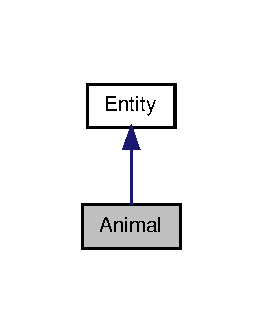
\includegraphics[width=126pt]{class_animal__inherit__graph}
\end{center}
\end{figure}


Collaboration diagram for Animal\-:
\nopagebreak
\begin{figure}[H]
\begin{center}
\leavevmode
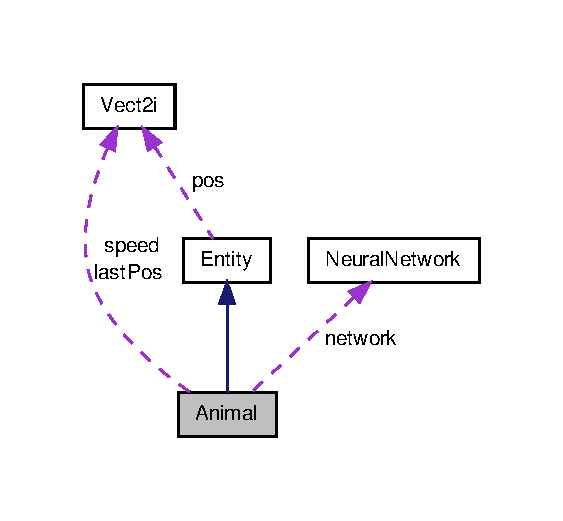
\includegraphics[width=270pt]{class_animal__coll__graph}
\end{center}
\end{figure}
\subsection*{Public Member Functions}
\begin{DoxyCompactItemize}
\item 
\hyperlink{class_animal_a1e726a49ec952443190ac62dad22353c}{Animal} ()
\item 
virtual \hyperlink{class_animal_a16d8b7f94611cc65f5cdb58cc105527b}{$\sim$\-Animal} ()
\item 
virtual void \hyperlink{class_animal_acd693bbac16d2f7dec930124887a9095}{init} ()
\begin{DoxyCompactList}\small\item\em Abstract method for object initialisation. \end{DoxyCompactList}\item 
void \hyperlink{class_animal_a75461b99c111f22dbb0231bcc397a1c9}{init} (const std\-::vector$<$ float $>$ \&D\-N\-A)
\begin{DoxyCompactList}\small\item\em Give new random position to the animal and set it's neural network's new D\-N\-A. \end{DoxyCompactList}\item 
void \hyperlink{class_animal_a18790d841ee27bf53ac8dfeb91750a80}{update} (const std\-::vector$<$ float $>$ inputs)
\begin{DoxyCompactList}\small\item\em Call the brain, giving it game inputs, to update the animal's state. \end{DoxyCompactList}\item 
void \hyperlink{class_animal_a31a4619f7b33b8b3ad6c0b1f43898cac}{increment\-Score} ()
\item 
void \hyperlink{class_animal_a557fe0d71dda75be2f8459ce0d7c2275}{die} ()
\item 
bool \hyperlink{class_animal_a5857d66a5303516578af7fc52ffc1107}{is\-Alive} () const 
\item 
int \hyperlink{class_animal_a9aedb2b6650341f976371a362d21ecfa}{get\-Score} () const 
\item 
int \hyperlink{class_animal_adabb251a3c5513ebbc62582a5a68055b}{get\-Closest\-Enemy\-Angle} () const 
\item 
int \hyperlink{class_animal_aac4b5d159b02fcae1dc6f427049c8485}{get\-Closest\-Fruit\-Angle} () const 
\item 
int \hyperlink{class_animal_a45483c0d3e22a02ca60aa83f4b1b0b23}{get\-Closest\-Ally\-Angle} () const 
\item 
float \hyperlink{class_animal_a49148f18eaebc09edf2bac4d3e44c7ea}{get\-Battle\-Output} () const 
\item 
float \hyperlink{class_animal_a757b167f05eafa17816598d4fcd2f184}{get\-Attack\-Value} () const 
\item 
float \hyperlink{class_animal_a00ec5bc73a90c26bfcf889fa5b85e688}{get\-Defense\-Value} () const 
\item 
\hyperlink{struct_vect2i}{Vect2i} \hyperlink{class_animal_a83a2929c3385a82aefaa689b3330c445}{get\-Display\-Pos} (const float \&interpolation) const 
\begin{DoxyCompactList}\small\item\em Return a intermediate position between old and new pos given the interpolation rate. \end{DoxyCompactList}\item 
std\-::vector$<$ float $>$ \hyperlink{class_animal_a0dcf09dfc831663b028a58a2c841dc06}{get\-D\-N\-A} ()
\begin{DoxyCompactList}\small\item\em Give the current network's D\-N\-A. \end{DoxyCompactList}\end{DoxyCompactItemize}
\subsection*{Protected Member Functions}
\begin{DoxyCompactItemize}
\item 
void \hyperlink{class_animal_a0b6103b76a223ce2eaad73877ff85c73}{update\-Position} (float da, float dp)
\begin{DoxyCompactList}\small\item\em Update the animal's position given 2 network outputs. \end{DoxyCompactList}\end{DoxyCompactItemize}
\subsection*{Protected Attributes}
\begin{DoxyCompactItemize}
\item 
\hyperlink{struct_vect2i}{Vect2i} \hyperlink{class_animal_a803f0b218477a5e365c1dde6128fb53e}{last\-Pos}
\item 
\hyperlink{struct_vect2i}{Vect2i} \hyperlink{class_animal_a280335c5deaf3402c85ab95a7653a483}{speed}
\item 
int \hyperlink{class_animal_ab5ab9a2e34464e0415b6588e820b0ad7}{score}
\item 
int \hyperlink{class_animal_a38e826603b1d70a75c89c59964d7e34e}{closest\-Enemy\-Angle}
\item 
int \hyperlink{class_animal_a587480ed32eadd3b7590e880f05d5e4d}{closest\-Fruit\-Angle}
\item 
int \hyperlink{class_animal_a53819180fe828fe2b68c7bbd7932ec9d}{closest\-Ally\-Angle}
\item 
float \hyperlink{class_animal_a3db09e6629852d9a54dc5b6648d3fb28}{battle\-Output}
\item 
bool \hyperlink{class_animal_a38d08d48cf5b16863bb40fa731b06629}{alive}
\item 
const int \hyperlink{class_animal_a4468a9e53e199e90deccd07d2315f13a}{A\-N\-I\-M\-A\-L\-\_\-\-L\-I\-N\-E\-A\-R\-\_\-\-S\-P\-E\-E\-D}
\item 
const int \hyperlink{class_animal_a4004efb93813a375712ad5d82a404659}{A\-N\-I\-M\-A\-L\-\_\-\-A\-N\-G\-U\-L\-A\-R\-\_\-\-S\-P\-E\-E\-D}
\item 
\hyperlink{class_neural_network}{Neural\-Network} \hyperlink{class_animal_a61e897a85af66b3b8315e313ed86a307}{network}
\end{DoxyCompactItemize}


\subsection{Detailed Description}
Class representing an animal, containing a brain (\hyperlink{class_neural_network}{Neural\-Network}), that changes the animal's state given game inputs. 

Definition at line 14 of file animal.\-h.



\subsection{Constructor \& Destructor Documentation}
\hypertarget{class_animal_a1e726a49ec952443190ac62dad22353c}{\index{Animal@{Animal}!Animal@{Animal}}
\index{Animal@{Animal}!Animal@{Animal}}
\subsubsection[{Animal}]{\setlength{\rightskip}{0pt plus 5cm}Animal\-::\-Animal (
\begin{DoxyParamCaption}
{}
\end{DoxyParamCaption}
)}}\label{class_animal_a1e726a49ec952443190ac62dad22353c}


Definition at line 5 of file animal.\-cpp.



Here is the call graph for this function\-:\nopagebreak
\begin{figure}[H]
\begin{center}
\leavevmode
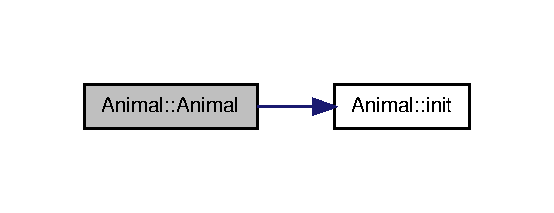
\includegraphics[width=266pt]{class_animal_a1e726a49ec952443190ac62dad22353c_cgraph}
\end{center}
\end{figure}


\hypertarget{class_animal_a16d8b7f94611cc65f5cdb58cc105527b}{\index{Animal@{Animal}!$\sim$\-Animal@{$\sim$\-Animal}}
\index{$\sim$\-Animal@{$\sim$\-Animal}!Animal@{Animal}}
\subsubsection[{$\sim$\-Animal}]{\setlength{\rightskip}{0pt plus 5cm}virtual Animal\-::$\sim$\-Animal (
\begin{DoxyParamCaption}
{}
\end{DoxyParamCaption}
)\hspace{0.3cm}{\ttfamily [inline]}, {\ttfamily [virtual]}}}\label{class_animal_a16d8b7f94611cc65f5cdb58cc105527b}


Definition at line 17 of file animal.\-h.



\subsection{Member Function Documentation}
\hypertarget{class_animal_a557fe0d71dda75be2f8459ce0d7c2275}{\index{Animal@{Animal}!die@{die}}
\index{die@{die}!Animal@{Animal}}
\subsubsection[{die}]{\setlength{\rightskip}{0pt plus 5cm}void Animal\-::die (
\begin{DoxyParamCaption}
{}
\end{DoxyParamCaption}
)}}\label{class_animal_a557fe0d71dda75be2f8459ce0d7c2275}


Definition at line 68 of file animal.\-cpp.

\hypertarget{class_animal_a757b167f05eafa17816598d4fcd2f184}{\index{Animal@{Animal}!get\-Attack\-Value@{get\-Attack\-Value}}
\index{get\-Attack\-Value@{get\-Attack\-Value}!Animal@{Animal}}
\subsubsection[{get\-Attack\-Value}]{\setlength{\rightskip}{0pt plus 5cm}float Animal\-::get\-Attack\-Value (
\begin{DoxyParamCaption}
{}
\end{DoxyParamCaption}
) const}}\label{class_animal_a757b167f05eafa17816598d4fcd2f184}
\begin{DoxyReturn}{Returns}
If battle\-Output $>$ 0, attack\-Value = battle\-Output 
\end{DoxyReturn}


Definition at line 72 of file animal.\-cpp.

\hypertarget{class_animal_a49148f18eaebc09edf2bac4d3e44c7ea}{\index{Animal@{Animal}!get\-Battle\-Output@{get\-Battle\-Output}}
\index{get\-Battle\-Output@{get\-Battle\-Output}!Animal@{Animal}}
\subsubsection[{get\-Battle\-Output}]{\setlength{\rightskip}{0pt plus 5cm}float Animal\-::get\-Battle\-Output (
\begin{DoxyParamCaption}
{}
\end{DoxyParamCaption}
) const\hspace{0.3cm}{\ttfamily [inline]}}}\label{class_animal_a49148f18eaebc09edf2bac4d3e44c7ea}


Definition at line 42 of file animal.\-h.

\hypertarget{class_animal_a45483c0d3e22a02ca60aa83f4b1b0b23}{\index{Animal@{Animal}!get\-Closest\-Ally\-Angle@{get\-Closest\-Ally\-Angle}}
\index{get\-Closest\-Ally\-Angle@{get\-Closest\-Ally\-Angle}!Animal@{Animal}}
\subsubsection[{get\-Closest\-Ally\-Angle}]{\setlength{\rightskip}{0pt plus 5cm}int Animal\-::get\-Closest\-Ally\-Angle (
\begin{DoxyParamCaption}
{}
\end{DoxyParamCaption}
) const\hspace{0.3cm}{\ttfamily [inline]}}}\label{class_animal_a45483c0d3e22a02ca60aa83f4b1b0b23}


Definition at line 41 of file animal.\-h.

\hypertarget{class_animal_adabb251a3c5513ebbc62582a5a68055b}{\index{Animal@{Animal}!get\-Closest\-Enemy\-Angle@{get\-Closest\-Enemy\-Angle}}
\index{get\-Closest\-Enemy\-Angle@{get\-Closest\-Enemy\-Angle}!Animal@{Animal}}
\subsubsection[{get\-Closest\-Enemy\-Angle}]{\setlength{\rightskip}{0pt plus 5cm}int Animal\-::get\-Closest\-Enemy\-Angle (
\begin{DoxyParamCaption}
{}
\end{DoxyParamCaption}
) const\hspace{0.3cm}{\ttfamily [inline]}}}\label{class_animal_adabb251a3c5513ebbc62582a5a68055b}


Definition at line 39 of file animal.\-h.

\hypertarget{class_animal_aac4b5d159b02fcae1dc6f427049c8485}{\index{Animal@{Animal}!get\-Closest\-Fruit\-Angle@{get\-Closest\-Fruit\-Angle}}
\index{get\-Closest\-Fruit\-Angle@{get\-Closest\-Fruit\-Angle}!Animal@{Animal}}
\subsubsection[{get\-Closest\-Fruit\-Angle}]{\setlength{\rightskip}{0pt plus 5cm}int Animal\-::get\-Closest\-Fruit\-Angle (
\begin{DoxyParamCaption}
{}
\end{DoxyParamCaption}
) const\hspace{0.3cm}{\ttfamily [inline]}}}\label{class_animal_aac4b5d159b02fcae1dc6f427049c8485}


Definition at line 40 of file animal.\-h.

\hypertarget{class_animal_a00ec5bc73a90c26bfcf889fa5b85e688}{\index{Animal@{Animal}!get\-Defense\-Value@{get\-Defense\-Value}}
\index{get\-Defense\-Value@{get\-Defense\-Value}!Animal@{Animal}}
\subsubsection[{get\-Defense\-Value}]{\setlength{\rightskip}{0pt plus 5cm}float Animal\-::get\-Defense\-Value (
\begin{DoxyParamCaption}
{}
\end{DoxyParamCaption}
) const}}\label{class_animal_a00ec5bc73a90c26bfcf889fa5b85e688}
\begin{DoxyReturn}{Returns}
If battle\-Output $<$ 0, defense\-Falue = -\/battle\-Output 
\end{DoxyReturn}


Definition at line 78 of file animal.\-cpp.

\hypertarget{class_animal_a83a2929c3385a82aefaa689b3330c445}{\index{Animal@{Animal}!get\-Display\-Pos@{get\-Display\-Pos}}
\index{get\-Display\-Pos@{get\-Display\-Pos}!Animal@{Animal}}
\subsubsection[{get\-Display\-Pos}]{\setlength{\rightskip}{0pt plus 5cm}{\bf Vect2i} Animal\-::get\-Display\-Pos (
\begin{DoxyParamCaption}
\item[{const float \&}]{interpolation}
\end{DoxyParamCaption}
) const}}\label{class_animal_a83a2929c3385a82aefaa689b3330c445}


Return a intermediate position between old and new pos given the interpolation rate. 


\begin{DoxyParams}{Parameters}
{\em interpolation} & The interpolation rate \\
\hline
\end{DoxyParams}
\begin{DoxyReturn}{Returns}
A 2\-D position between old and new pos 
\end{DoxyReturn}


Definition at line 89 of file animal.\-cpp.

\hypertarget{class_animal_a0dcf09dfc831663b028a58a2c841dc06}{\index{Animal@{Animal}!get\-D\-N\-A@{get\-D\-N\-A}}
\index{get\-D\-N\-A@{get\-D\-N\-A}!Animal@{Animal}}
\subsubsection[{get\-D\-N\-A}]{\setlength{\rightskip}{0pt plus 5cm}std\-::vector$<$ float $>$ Animal\-::get\-D\-N\-A (
\begin{DoxyParamCaption}
{}
\end{DoxyParamCaption}
)}}\label{class_animal_a0dcf09dfc831663b028a58a2c841dc06}


Give the current network's D\-N\-A. 

\begin{DoxyReturn}{Returns}
The current animal's N\-N D\-N\-A 
\end{DoxyReturn}


Definition at line 119 of file animal.\-cpp.



Here is the call graph for this function\-:\nopagebreak
\begin{figure}[H]
\begin{center}
\leavevmode
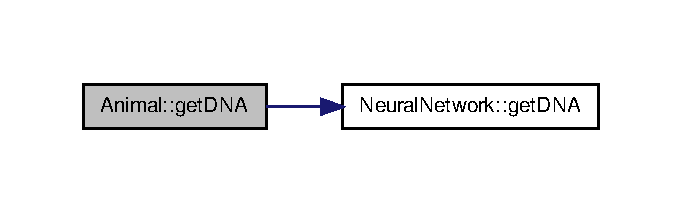
\includegraphics[width=328pt]{class_animal_a0dcf09dfc831663b028a58a2c841dc06_cgraph}
\end{center}
\end{figure}


\hypertarget{class_animal_a9aedb2b6650341f976371a362d21ecfa}{\index{Animal@{Animal}!get\-Score@{get\-Score}}
\index{get\-Score@{get\-Score}!Animal@{Animal}}
\subsubsection[{get\-Score}]{\setlength{\rightskip}{0pt plus 5cm}int Animal\-::get\-Score (
\begin{DoxyParamCaption}
{}
\end{DoxyParamCaption}
) const\hspace{0.3cm}{\ttfamily [inline]}}}\label{class_animal_a9aedb2b6650341f976371a362d21ecfa}


Definition at line 38 of file animal.\-h.

\hypertarget{class_animal_a31a4619f7b33b8b3ad6c0b1f43898cac}{\index{Animal@{Animal}!increment\-Score@{increment\-Score}}
\index{increment\-Score@{increment\-Score}!Animal@{Animal}}
\subsubsection[{increment\-Score}]{\setlength{\rightskip}{0pt plus 5cm}void Animal\-::increment\-Score (
\begin{DoxyParamCaption}
{}
\end{DoxyParamCaption}
)}}\label{class_animal_a31a4619f7b33b8b3ad6c0b1f43898cac}


Definition at line 64 of file animal.\-cpp.

\hypertarget{class_animal_acd693bbac16d2f7dec930124887a9095}{\index{Animal@{Animal}!init@{init}}
\index{init@{init}!Animal@{Animal}}
\subsubsection[{init}]{\setlength{\rightskip}{0pt plus 5cm}void Animal\-::init (
\begin{DoxyParamCaption}
{}
\end{DoxyParamCaption}
)\hspace{0.3cm}{\ttfamily [virtual]}}}\label{class_animal_acd693bbac16d2f7dec930124887a9095}


Abstract method for object initialisation. 



Implements \hyperlink{class_entity_a31e6183ea44922d54a43be48b8fd4bc0}{Entity}.



Definition at line 12 of file animal.\-cpp.



Here is the caller graph for this function\-:\nopagebreak
\begin{figure}[H]
\begin{center}
\leavevmode
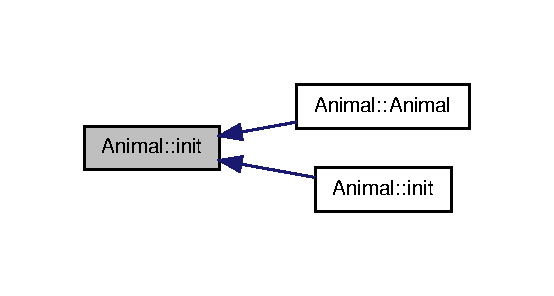
\includegraphics[width=266pt]{class_animal_acd693bbac16d2f7dec930124887a9095_icgraph}
\end{center}
\end{figure}


\hypertarget{class_animal_a75461b99c111f22dbb0231bcc397a1c9}{\index{Animal@{Animal}!init@{init}}
\index{init@{init}!Animal@{Animal}}
\subsubsection[{init}]{\setlength{\rightskip}{0pt plus 5cm}void Animal\-::init (
\begin{DoxyParamCaption}
\item[{const std\-::vector$<$ float $>$ \&}]{D\-N\-A}
\end{DoxyParamCaption}
)}}\label{class_animal_a75461b99c111f22dbb0231bcc397a1c9}


Give new random position to the animal and set it's neural network's new D\-N\-A. 


\begin{DoxyParams}{Parameters}
{\em D\-N\-A} & The new D\-N\-A to give to the \hyperlink{class_neural_network}{Neural\-Network} \\
\hline
\end{DoxyParams}


Definition at line 27 of file animal.\-cpp.



Here is the call graph for this function\-:\nopagebreak
\begin{figure}[H]
\begin{center}
\leavevmode
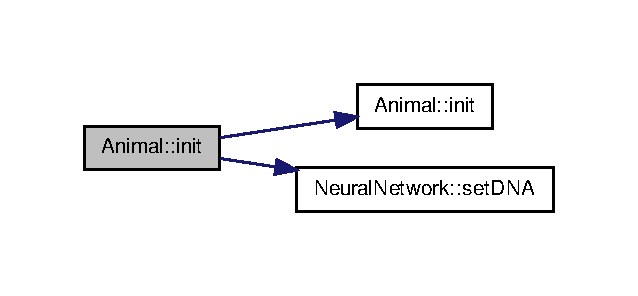
\includegraphics[width=306pt]{class_animal_a75461b99c111f22dbb0231bcc397a1c9_cgraph}
\end{center}
\end{figure}


\hypertarget{class_animal_a5857d66a5303516578af7fc52ffc1107}{\index{Animal@{Animal}!is\-Alive@{is\-Alive}}
\index{is\-Alive@{is\-Alive}!Animal@{Animal}}
\subsubsection[{is\-Alive}]{\setlength{\rightskip}{0pt plus 5cm}bool Animal\-::is\-Alive (
\begin{DoxyParamCaption}
{}
\end{DoxyParamCaption}
) const\hspace{0.3cm}{\ttfamily [inline]}}}\label{class_animal_a5857d66a5303516578af7fc52ffc1107}


Definition at line 37 of file animal.\-h.



Here is the caller graph for this function\-:\nopagebreak
\begin{figure}[H]
\begin{center}
\leavevmode
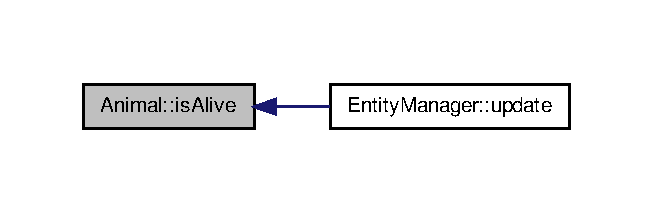
\includegraphics[width=314pt]{class_animal_a5857d66a5303516578af7fc52ffc1107_icgraph}
\end{center}
\end{figure}


\hypertarget{class_animal_a18790d841ee27bf53ac8dfeb91750a80}{\index{Animal@{Animal}!update@{update}}
\index{update@{update}!Animal@{Animal}}
\subsubsection[{update}]{\setlength{\rightskip}{0pt plus 5cm}void Animal\-::update (
\begin{DoxyParamCaption}
\item[{const std\-::vector$<$ float $>$}]{inputs}
\end{DoxyParamCaption}
)}}\label{class_animal_a18790d841ee27bf53ac8dfeb91750a80}


Call the brain, giving it game inputs, to update the animal's state. 


\begin{DoxyParams}{Parameters}
{\em inputs} & The game inputs to give to the N\-N \\
\hline
\end{DoxyParams}


Definition at line 33 of file animal.\-cpp.



Here is the call graph for this function\-:\nopagebreak
\begin{figure}[H]
\begin{center}
\leavevmode
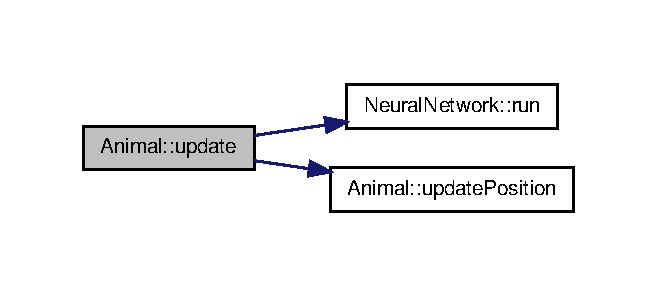
\includegraphics[width=316pt]{class_animal_a18790d841ee27bf53ac8dfeb91750a80_cgraph}
\end{center}
\end{figure}


\hypertarget{class_animal_a0b6103b76a223ce2eaad73877ff85c73}{\index{Animal@{Animal}!update\-Position@{update\-Position}}
\index{update\-Position@{update\-Position}!Animal@{Animal}}
\subsubsection[{update\-Position}]{\setlength{\rightskip}{0pt plus 5cm}void Animal\-::update\-Position (
\begin{DoxyParamCaption}
\item[{float}]{da, }
\item[{float}]{dp}
\end{DoxyParamCaption}
)\hspace{0.3cm}{\ttfamily [protected]}}}\label{class_animal_a0b6103b76a223ce2eaad73877ff85c73}


Update the animal's position given 2 network outputs. 


\begin{DoxyParams}{Parameters}
{\em da} & \mbox{[}-\/1; 1\mbox{]} value representing the angular difference between old and new pos \\
\hline
{\em dp} & \mbox{[}-\/1; 1\mbox{]} value representing the linear difference between old and new pos \\
\hline
\end{DoxyParams}


Definition at line 94 of file animal.\-cpp.



Here is the caller graph for this function\-:\nopagebreak
\begin{figure}[H]
\begin{center}
\leavevmode
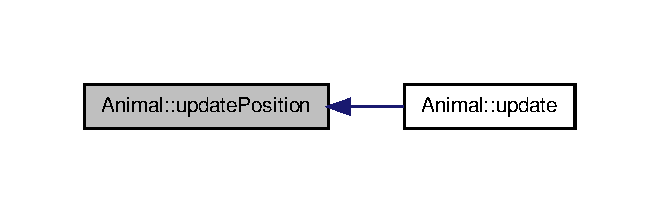
\includegraphics[width=316pt]{class_animal_a0b6103b76a223ce2eaad73877ff85c73_icgraph}
\end{center}
\end{figure}




\subsection{Member Data Documentation}
\hypertarget{class_animal_a38d08d48cf5b16863bb40fa731b06629}{\index{Animal@{Animal}!alive@{alive}}
\index{alive@{alive}!Animal@{Animal}}
\subsubsection[{alive}]{\setlength{\rightskip}{0pt plus 5cm}bool Animal\-::alive\hspace{0.3cm}{\ttfamily [protected]}}}\label{class_animal_a38d08d48cf5b16863bb40fa731b06629}


Definition at line 81 of file animal.\-h.

\hypertarget{class_animal_a4004efb93813a375712ad5d82a404659}{\index{Animal@{Animal}!A\-N\-I\-M\-A\-L\-\_\-\-A\-N\-G\-U\-L\-A\-R\-\_\-\-S\-P\-E\-E\-D@{A\-N\-I\-M\-A\-L\-\_\-\-A\-N\-G\-U\-L\-A\-R\-\_\-\-S\-P\-E\-E\-D}}
\index{A\-N\-I\-M\-A\-L\-\_\-\-A\-N\-G\-U\-L\-A\-R\-\_\-\-S\-P\-E\-E\-D@{A\-N\-I\-M\-A\-L\-\_\-\-A\-N\-G\-U\-L\-A\-R\-\_\-\-S\-P\-E\-E\-D}!Animal@{Animal}}
\subsubsection[{A\-N\-I\-M\-A\-L\-\_\-\-A\-N\-G\-U\-L\-A\-R\-\_\-\-S\-P\-E\-E\-D}]{\setlength{\rightskip}{0pt plus 5cm}const int Animal\-::\-A\-N\-I\-M\-A\-L\-\_\-\-A\-N\-G\-U\-L\-A\-R\-\_\-\-S\-P\-E\-E\-D\hspace{0.3cm}{\ttfamily [protected]}}}\label{class_animal_a4004efb93813a375712ad5d82a404659}


Definition at line 83 of file animal.\-h.

\hypertarget{class_animal_a4468a9e53e199e90deccd07d2315f13a}{\index{Animal@{Animal}!A\-N\-I\-M\-A\-L\-\_\-\-L\-I\-N\-E\-A\-R\-\_\-\-S\-P\-E\-E\-D@{A\-N\-I\-M\-A\-L\-\_\-\-L\-I\-N\-E\-A\-R\-\_\-\-S\-P\-E\-E\-D}}
\index{A\-N\-I\-M\-A\-L\-\_\-\-L\-I\-N\-E\-A\-R\-\_\-\-S\-P\-E\-E\-D@{A\-N\-I\-M\-A\-L\-\_\-\-L\-I\-N\-E\-A\-R\-\_\-\-S\-P\-E\-E\-D}!Animal@{Animal}}
\subsubsection[{A\-N\-I\-M\-A\-L\-\_\-\-L\-I\-N\-E\-A\-R\-\_\-\-S\-P\-E\-E\-D}]{\setlength{\rightskip}{0pt plus 5cm}const int Animal\-::\-A\-N\-I\-M\-A\-L\-\_\-\-L\-I\-N\-E\-A\-R\-\_\-\-S\-P\-E\-E\-D\hspace{0.3cm}{\ttfamily [protected]}}}\label{class_animal_a4468a9e53e199e90deccd07d2315f13a}


Definition at line 83 of file animal.\-h.

\hypertarget{class_animal_a3db09e6629852d9a54dc5b6648d3fb28}{\index{Animal@{Animal}!battle\-Output@{battle\-Output}}
\index{battle\-Output@{battle\-Output}!Animal@{Animal}}
\subsubsection[{battle\-Output}]{\setlength{\rightskip}{0pt plus 5cm}float Animal\-::battle\-Output\hspace{0.3cm}{\ttfamily [protected]}}}\label{class_animal_a3db09e6629852d9a54dc5b6648d3fb28}


Definition at line 79 of file animal.\-h.

\hypertarget{class_animal_a53819180fe828fe2b68c7bbd7932ec9d}{\index{Animal@{Animal}!closest\-Ally\-Angle@{closest\-Ally\-Angle}}
\index{closest\-Ally\-Angle@{closest\-Ally\-Angle}!Animal@{Animal}}
\subsubsection[{closest\-Ally\-Angle}]{\setlength{\rightskip}{0pt plus 5cm}int Animal\-::closest\-Ally\-Angle\hspace{0.3cm}{\ttfamily [protected]}}}\label{class_animal_a53819180fe828fe2b68c7bbd7932ec9d}


Definition at line 76 of file animal.\-h.

\hypertarget{class_animal_a38e826603b1d70a75c89c59964d7e34e}{\index{Animal@{Animal}!closest\-Enemy\-Angle@{closest\-Enemy\-Angle}}
\index{closest\-Enemy\-Angle@{closest\-Enemy\-Angle}!Animal@{Animal}}
\subsubsection[{closest\-Enemy\-Angle}]{\setlength{\rightskip}{0pt plus 5cm}int Animal\-::closest\-Enemy\-Angle\hspace{0.3cm}{\ttfamily [protected]}}}\label{class_animal_a38e826603b1d70a75c89c59964d7e34e}


Definition at line 76 of file animal.\-h.

\hypertarget{class_animal_a587480ed32eadd3b7590e880f05d5e4d}{\index{Animal@{Animal}!closest\-Fruit\-Angle@{closest\-Fruit\-Angle}}
\index{closest\-Fruit\-Angle@{closest\-Fruit\-Angle}!Animal@{Animal}}
\subsubsection[{closest\-Fruit\-Angle}]{\setlength{\rightskip}{0pt plus 5cm}int Animal\-::closest\-Fruit\-Angle\hspace{0.3cm}{\ttfamily [protected]}}}\label{class_animal_a587480ed32eadd3b7590e880f05d5e4d}


Definition at line 76 of file animal.\-h.

\hypertarget{class_animal_a803f0b218477a5e365c1dde6128fb53e}{\index{Animal@{Animal}!last\-Pos@{last\-Pos}}
\index{last\-Pos@{last\-Pos}!Animal@{Animal}}
\subsubsection[{last\-Pos}]{\setlength{\rightskip}{0pt plus 5cm}{\bf Vect2i} Animal\-::last\-Pos\hspace{0.3cm}{\ttfamily [protected]}}}\label{class_animal_a803f0b218477a5e365c1dde6128fb53e}


Definition at line 73 of file animal.\-h.

\hypertarget{class_animal_a61e897a85af66b3b8315e313ed86a307}{\index{Animal@{Animal}!network@{network}}
\index{network@{network}!Animal@{Animal}}
\subsubsection[{network}]{\setlength{\rightskip}{0pt plus 5cm}{\bf Neural\-Network} Animal\-::network\hspace{0.3cm}{\ttfamily [protected]}}}\label{class_animal_a61e897a85af66b3b8315e313ed86a307}


Definition at line 85 of file animal.\-h.

\hypertarget{class_animal_ab5ab9a2e34464e0415b6588e820b0ad7}{\index{Animal@{Animal}!score@{score}}
\index{score@{score}!Animal@{Animal}}
\subsubsection[{score}]{\setlength{\rightskip}{0pt plus 5cm}int Animal\-::score\hspace{0.3cm}{\ttfamily [protected]}}}\label{class_animal_ab5ab9a2e34464e0415b6588e820b0ad7}


Definition at line 75 of file animal.\-h.

\hypertarget{class_animal_a280335c5deaf3402c85ab95a7653a483}{\index{Animal@{Animal}!speed@{speed}}
\index{speed@{speed}!Animal@{Animal}}
\subsubsection[{speed}]{\setlength{\rightskip}{0pt plus 5cm}{\bf Vect2i} Animal\-::speed\hspace{0.3cm}{\ttfamily [protected]}}}\label{class_animal_a280335c5deaf3402c85ab95a7653a483}


Definition at line 73 of file animal.\-h.



The documentation for this class was generated from the following files\-:\begin{DoxyCompactItemize}
\item 
src/\hyperlink{animal_8h}{animal.\-h}\item 
src/\hyperlink{animal_8cpp}{animal.\-cpp}\end{DoxyCompactItemize}

\hypertarget{struct_bush}{\section{Bush Struct Reference}
\label{struct_bush}\index{Bush@{Bush}}
}


Structure representig a bush \-: point and size where fruits have high probabylity to appear.  




{\ttfamily \#include $<$fruit.\-h$>$}



Collaboration diagram for Bush\-:
\nopagebreak
\begin{figure}[H]
\begin{center}
\leavevmode
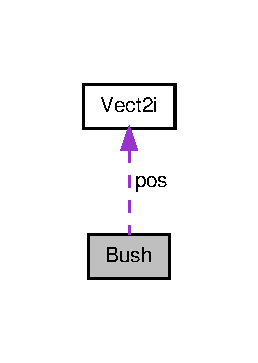
\includegraphics[width=124pt]{struct_bush__coll__graph}
\end{center}
\end{figure}
\subsection*{Public Attributes}
\begin{DoxyCompactItemize}
\item 
\hyperlink{struct_vect2i}{Vect2i} \hyperlink{struct_bush_ab3135be5ff260f0e223cb9c64f4aedc3}{pos}
\begin{DoxyCompactList}\small\item\em Center of the bush. \end{DoxyCompactList}\item 
int \hyperlink{struct_bush_a3b40c2cda3c709539246d302e74b8168}{size}
\begin{DoxyCompactList}\small\item\em size of the bush (to be used in a gaussian probability function) \end{DoxyCompactList}\end{DoxyCompactItemize}


\subsection{Detailed Description}
Structure representig a bush \-: point and size where fruits have high probabylity to appear. 

It is used to make fruits appear in a realistic way, ie in the form of bushes of different sizes all around the world. You can play around with it by changing Bushes\-Number, Bushes\-Min\-Size and Bushes\-Max\-Size in config.\-cfg 

Definition at line 15 of file fruit.\-h.



\subsection{Member Data Documentation}
\hypertarget{struct_bush_ab3135be5ff260f0e223cb9c64f4aedc3}{\index{Bush@{Bush}!pos@{pos}}
\index{pos@{pos}!Bush@{Bush}}
\subsubsection[{pos}]{\setlength{\rightskip}{0pt plus 5cm}{\bf Vect2i} Bush\-::pos}}\label{struct_bush_ab3135be5ff260f0e223cb9c64f4aedc3}


Center of the bush. 



Definition at line 16 of file fruit.\-h.

\hypertarget{struct_bush_a3b40c2cda3c709539246d302e74b8168}{\index{Bush@{Bush}!size@{size}}
\index{size@{size}!Bush@{Bush}}
\subsubsection[{size}]{\setlength{\rightskip}{0pt plus 5cm}int Bush\-::size}}\label{struct_bush_a3b40c2cda3c709539246d302e74b8168}


size of the bush (to be used in a gaussian probability function) 



Definition at line 17 of file fruit.\-h.



The documentation for this struct was generated from the following file\-:\begin{DoxyCompactItemize}
\item 
src/\hyperlink{fruit_8h}{fruit.\-h}\end{DoxyCompactItemize}

\hypertarget{class_config_parser}{\section{Config\-Parser Class Reference}
\label{class_config_parser}\index{Config\-Parser@{Config\-Parser}}
}


{\ttfamily \#include $<$config\-\_\-parser.\-h$>$}

\subsection*{Public Member Functions}
\begin{DoxyCompactItemize}
\item 
int \hyperlink{class_config_parser_a9eb8031a0252a34fcb808dba2b9780e5}{read\-Int} (const std\-::string \&key, const int \&default\-Value=0) const 
\item 
float \hyperlink{class_config_parser_a7a4b723bc0f88e966f4b67347b5264cd}{read\-Float} (const std\-::string \&key, const float \&default\-Value=0.f) const 
\item 
std\-::string \hyperlink{class_config_parser_abcdb07fdc295e07adefbd338c552c493}{read\-String} (const std\-::string \&key, const std\-::string \&default\-Value=\char`\"{}\char`\"{}) const 
\item 
void \hyperlink{class_config_parser_a49ddd20e2f9ea0ea864c3006d2177323}{set\-Int} (const std\-::string \&key, const int \&value)
\item 
void \hyperlink{class_config_parser_a18ad19fa692a557be50d868fd3f83ca3}{set\-Float} (const std\-::string \&key, const float \&value)
\item 
void \hyperlink{class_config_parser_a6eba995aa9d58ad843d05e3f0a003d3e}{set\-String} (const std\-::string \&key, const std\-::string \&value)
\item 
void \hyperlink{class_config_parser_adcaa724f20085403bb1beb7918903fdd}{read\-File} (const std\-::string \&file\-Name)
\item 
void \hyperlink{class_config_parser_a98928657410a8c91f9d68c5d5235ace1}{save\-File} (const std\-::string \&file\-Name=\char`\"{}\char`\"{})
\end{DoxyCompactItemize}
\subsection*{Static Public Member Functions}
\begin{DoxyCompactItemize}
\item 
static void \hyperlink{class_config_parser_a7525ed2717618bab9644cec9cb77bbdd}{create} (const std\-::string \&file\-Name=\char`\"{}\char`\"{})
\item 
static void \hyperlink{class_config_parser_a2c271ec9f6b7f5182c6781a56514f1ef}{kill} ()
\item 
static \hyperlink{class_config_parser}{Config\-Parser} $\ast$ \hyperlink{class_config_parser_a3d3cbdae938afd36cffd28561830d1af}{get} ()
\end{DoxyCompactItemize}


\subsection{Detailed Description}

<<<<<<< HEAD

Definition at line 20 of file config\-\_\-parser.\-h.
=======
\begin{DoxyParams}{Parameters}
{\em file\-Name} & Utility singleton class parsing a config file (default 'files/config.\-cfg') that contains constants used by a project, organized by type (int, float, string), referenced by their name and stored in maps.\\
\hline
\end{DoxyParams}
I wrote this class a long time ago, to allow me to quickly change any constant int/float/string without recompiling every time. Using maps, it can be quite long to process when called a lot. This is why I save all constants in private const in every class I use them. I won't discuss its inner working, as it is oooooold. 

Definition at line 22 of file config\-\_\-parser.\-h.
>>>>>>> master



\subsection{Member Function Documentation}
\hypertarget{class_config_parser_a7525ed2717618bab9644cec9cb77bbdd}{\index{Config\-Parser@{Config\-Parser}!create@{create}}
\index{create@{create}!ConfigParser@{Config\-Parser}}
\subsubsection[{create}]{\setlength{\rightskip}{0pt plus 5cm}void Config\-Parser\-::create (
\begin{DoxyParamCaption}
\item[{const std\-::string \&}]{file\-Name = {\ttfamily \char`\"{}\char`\"{}}}
\end{DoxyParamCaption}
)\hspace{0.3cm}{\ttfamily [static]}}}\label{class_config_parser_a7525ed2717618bab9644cec9cb77bbdd}


Definition at line 8 of file config\-\_\-parser.\-cpp.

\hypertarget{class_config_parser_a3d3cbdae938afd36cffd28561830d1af}{\index{Config\-Parser@{Config\-Parser}!get@{get}}
\index{get@{get}!ConfigParser@{Config\-Parser}}
\subsubsection[{get}]{\setlength{\rightskip}{0pt plus 5cm}{\bf Config\-Parser} $\ast$ Config\-Parser\-::get (
\begin{DoxyParamCaption}
{}
\end{DoxyParamCaption}
)\hspace{0.3cm}{\ttfamily [static]}}}\label{class_config_parser_a3d3cbdae938afd36cffd28561830d1af}


Definition at line 15 of file config\-\_\-parser.\-cpp.

\hypertarget{class_config_parser_a2c271ec9f6b7f5182c6781a56514f1ef}{\index{Config\-Parser@{Config\-Parser}!kill@{kill}}
\index{kill@{kill}!ConfigParser@{Config\-Parser}}
\subsubsection[{kill}]{\setlength{\rightskip}{0pt plus 5cm}void Config\-Parser\-::kill (
\begin{DoxyParamCaption}
{}
\end{DoxyParamCaption}
)\hspace{0.3cm}{\ttfamily [static]}}}\label{class_config_parser_a2c271ec9f6b7f5182c6781a56514f1ef}


Definition at line 14 of file config\-\_\-parser.\-cpp.

\hypertarget{class_config_parser_adcaa724f20085403bb1beb7918903fdd}{\index{Config\-Parser@{Config\-Parser}!read\-File@{read\-File}}
\index{read\-File@{read\-File}!ConfigParser@{Config\-Parser}}
\subsubsection[{read\-File}]{\setlength{\rightskip}{0pt plus 5cm}void Config\-Parser\-::read\-File (
\begin{DoxyParamCaption}
\item[{const std\-::string \&}]{file\-Name}
\end{DoxyParamCaption}
)}}\label{class_config_parser_adcaa724f20085403bb1beb7918903fdd}


Definition at line 85 of file config\-\_\-parser.\-cpp.

\hypertarget{class_config_parser_a7a4b723bc0f88e966f4b67347b5264cd}{\index{Config\-Parser@{Config\-Parser}!read\-Float@{read\-Float}}
\index{read\-Float@{read\-Float}!ConfigParser@{Config\-Parser}}
\subsubsection[{read\-Float}]{\setlength{\rightskip}{0pt plus 5cm}float Config\-Parser\-::read\-Float (
\begin{DoxyParamCaption}
\item[{const std\-::string \&}]{key, }
\item[{const float \&}]{default\-Value = {\ttfamily 0.f}}
\end{DoxyParamCaption}
) const}}\label{class_config_parser_a7a4b723bc0f88e966f4b67347b5264cd}


Definition at line 43 of file config\-\_\-parser.\-cpp.

\hypertarget{class_config_parser_a9eb8031a0252a34fcb808dba2b9780e5}{\index{Config\-Parser@{Config\-Parser}!read\-Int@{read\-Int}}
\index{read\-Int@{read\-Int}!ConfigParser@{Config\-Parser}}
\subsubsection[{read\-Int}]{\setlength{\rightskip}{0pt plus 5cm}int Config\-Parser\-::read\-Int (
\begin{DoxyParamCaption}
\item[{const std\-::string \&}]{key, }
\item[{const int \&}]{default\-Value = {\ttfamily 0}}
\end{DoxyParamCaption}
) const}}\label{class_config_parser_a9eb8031a0252a34fcb808dba2b9780e5}


Definition at line 36 of file config\-\_\-parser.\-cpp.

\hypertarget{class_config_parser_abcdb07fdc295e07adefbd338c552c493}{\index{Config\-Parser@{Config\-Parser}!read\-String@{read\-String}}
\index{read\-String@{read\-String}!ConfigParser@{Config\-Parser}}
\subsubsection[{read\-String}]{\setlength{\rightskip}{0pt plus 5cm}string Config\-Parser\-::read\-String (
\begin{DoxyParamCaption}
\item[{const std\-::string \&}]{key, }
\item[{const std\-::string \&}]{default\-Value = {\ttfamily \char`\"{}\char`\"{}}}
\end{DoxyParamCaption}
) const}}\label{class_config_parser_abcdb07fdc295e07adefbd338c552c493}


Definition at line 50 of file config\-\_\-parser.\-cpp.

\hypertarget{class_config_parser_a98928657410a8c91f9d68c5d5235ace1}{\index{Config\-Parser@{Config\-Parser}!save\-File@{save\-File}}
\index{save\-File@{save\-File}!ConfigParser@{Config\-Parser}}
\subsubsection[{save\-File}]{\setlength{\rightskip}{0pt plus 5cm}void Config\-Parser\-::save\-File (
\begin{DoxyParamCaption}
\item[{const std\-::string \&}]{file\-Name = {\ttfamily \char`\"{}\char`\"{}}}
\end{DoxyParamCaption}
)}}\label{class_config_parser_a98928657410a8c91f9d68c5d5235ace1}


Definition at line 182 of file config\-\_\-parser.\-cpp.

\hypertarget{class_config_parser_a18ad19fa692a557be50d868fd3f83ca3}{\index{Config\-Parser@{Config\-Parser}!set\-Float@{set\-Float}}
\index{set\-Float@{set\-Float}!ConfigParser@{Config\-Parser}}
\subsubsection[{set\-Float}]{\setlength{\rightskip}{0pt plus 5cm}void Config\-Parser\-::set\-Float (
\begin{DoxyParamCaption}
\item[{const std\-::string \&}]{key, }
\item[{const float \&}]{value}
\end{DoxyParamCaption}
)}}\label{class_config_parser_a18ad19fa692a557be50d868fd3f83ca3}


Definition at line 67 of file config\-\_\-parser.\-cpp.

\hypertarget{class_config_parser_a49ddd20e2f9ea0ea864c3006d2177323}{\index{Config\-Parser@{Config\-Parser}!set\-Int@{set\-Int}}
\index{set\-Int@{set\-Int}!ConfigParser@{Config\-Parser}}
\subsubsection[{set\-Int}]{\setlength{\rightskip}{0pt plus 5cm}void Config\-Parser\-::set\-Int (
\begin{DoxyParamCaption}
\item[{const std\-::string \&}]{key, }
\item[{const int \&}]{value}
\end{DoxyParamCaption}
)}}\label{class_config_parser_a49ddd20e2f9ea0ea864c3006d2177323}


Definition at line 58 of file config\-\_\-parser.\-cpp.

\hypertarget{class_config_parser_a6eba995aa9d58ad843d05e3f0a003d3e}{\index{Config\-Parser@{Config\-Parser}!set\-String@{set\-String}}
\index{set\-String@{set\-String}!ConfigParser@{Config\-Parser}}
\subsubsection[{set\-String}]{\setlength{\rightskip}{0pt plus 5cm}void Config\-Parser\-::set\-String (
\begin{DoxyParamCaption}
\item[{const std\-::string \&}]{key, }
\item[{const std\-::string \&}]{value}
\end{DoxyParamCaption}
)}}\label{class_config_parser_a6eba995aa9d58ad843d05e3f0a003d3e}


Definition at line 76 of file config\-\_\-parser.\-cpp.



The documentation for this class was generated from the following files\-:\begin{DoxyCompactItemize}
\item 
src/\hyperlink{config__parser_8h}{config\-\_\-parser.\-h}\item 
src/\hyperlink{config__parser_8cpp}{config\-\_\-parser.\-cpp}\end{DoxyCompactItemize}

\hypertarget{class_display}{\section{Display Class Reference}
\label{class_display}\index{Display@{Display}}
}


Class handling every display aspect of the game.  




{\ttfamily \#include $<$display.\-h$>$}

\subsection*{Public Member Functions}
\begin{DoxyCompactItemize}
\item 
\hyperlink{class_display_a21052a50c5e922272d697aaf5cfb14cc}{Display} (\hyperlink{class_game}{Game} $\ast$\-\_\-game)
\item 
\hyperlink{class_display_ac2607a6bb236c55547a4223d40d85d1f}{$\sim$\-Display} ()
\item 
void \hyperlink{class_display_a713ee81045f32895c2b063037c81c388}{update} (const \hyperlink{class_entity_manager}{Entity\-Manager} \&manager, const float \&\-\_\-interpolation)
\begin{DoxyCompactList}\small\item\em Displays all the game elements and the U\-I. \end{DoxyCompactList}\item 
void \hyperlink{class_display_a05ee6cd33afcc51a5856148677a71c82}{events} ()
\begin{DoxyCompactList}\small\item\em Handles all the user events. \end{DoxyCompactList}\end{DoxyCompactItemize}


\subsection{Detailed Description}
Class handling every display aspect of the game. 


\begin{DoxyParams}{Parameters}
{\em \-\_\-game} & Ptr to its parent game object \\
\hline
\end{DoxyParams}


Definition at line 20 of file display.\-h.



\subsection{Constructor \& Destructor Documentation}
\hypertarget{class_display_a21052a50c5e922272d697aaf5cfb14cc}{\index{Display@{Display}!Display@{Display}}
\index{Display@{Display}!Display@{Display}}
\subsubsection[{Display}]{\setlength{\rightskip}{0pt plus 5cm}Display\-::\-Display (
\begin{DoxyParamCaption}
\item[{{\bf Game} $\ast$}]{\-\_\-game}
\end{DoxyParamCaption}
)}}\label{class_display_a21052a50c5e922272d697aaf5cfb14cc}


Definition at line 5 of file display.\-cpp.

\hypertarget{class_display_ac2607a6bb236c55547a4223d40d85d1f}{\index{Display@{Display}!$\sim$\-Display@{$\sim$\-Display}}
\index{$\sim$\-Display@{$\sim$\-Display}!Display@{Display}}
\subsubsection[{$\sim$\-Display}]{\setlength{\rightskip}{0pt plus 5cm}Display\-::$\sim$\-Display (
\begin{DoxyParamCaption}
{}
\end{DoxyParamCaption}
)\hspace{0.3cm}{\ttfamily [inline]}}}\label{class_display_ac2607a6bb236c55547a4223d40d85d1f}


Definition at line 24 of file display.\-h.



\subsection{Member Function Documentation}
\hypertarget{class_display_a05ee6cd33afcc51a5856148677a71c82}{\index{Display@{Display}!events@{events}}
\index{events@{events}!Display@{Display}}
\subsubsection[{events}]{\setlength{\rightskip}{0pt plus 5cm}void Display\-::events (
\begin{DoxyParamCaption}
{}
\end{DoxyParamCaption}
)}}\label{class_display_a05ee6cd33afcc51a5856148677a71c82}


Handles all the user events. 



Definition at line 54 of file display.\-cpp.



Here is the call graph for this function\-:\nopagebreak
\begin{figure}[H]
\begin{center}
\leavevmode
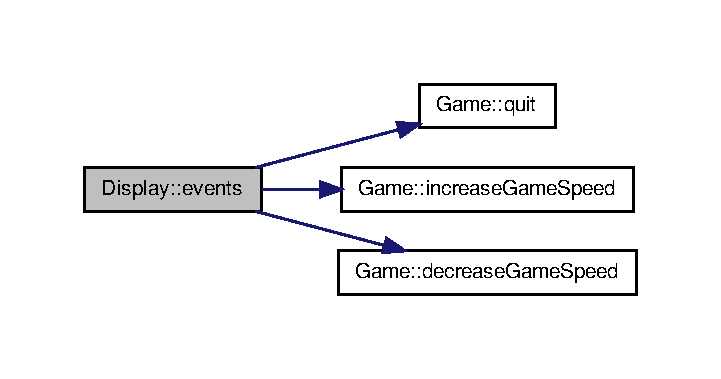
\includegraphics[width=346pt]{class_display_a05ee6cd33afcc51a5856148677a71c82_cgraph}
\end{center}
\end{figure}




Here is the caller graph for this function\-:\nopagebreak
\begin{figure}[H]
\begin{center}
\leavevmode
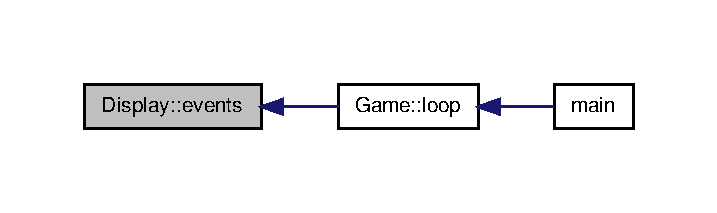
\includegraphics[width=344pt]{class_display_a05ee6cd33afcc51a5856148677a71c82_icgraph}
\end{center}
\end{figure}


\hypertarget{class_display_a713ee81045f32895c2b063037c81c388}{\index{Display@{Display}!update@{update}}
\index{update@{update}!Display@{Display}}
\subsubsection[{update}]{\setlength{\rightskip}{0pt plus 5cm}void Display\-::update (
\begin{DoxyParamCaption}
\item[{const {\bf Entity\-Manager} \&}]{manager, }
\item[{const float \&}]{\-\_\-interpolation}
\end{DoxyParamCaption}
)}}\label{class_display_a713ee81045f32895c2b063037c81c388}


Displays all the game elements and the U\-I. 


\begin{DoxyParams}{Parameters}
{\em manager} & Reference to the manager containing all entities to be displayed \\
\hline
{\em \-\_\-interpolation} & Rate describing the interval of time between 2 game updates \\
\hline
\end{DoxyParams}


Definition at line 41 of file display.\-cpp.



Here is the caller graph for this function\-:\nopagebreak
\begin{figure}[H]
\begin{center}
\leavevmode
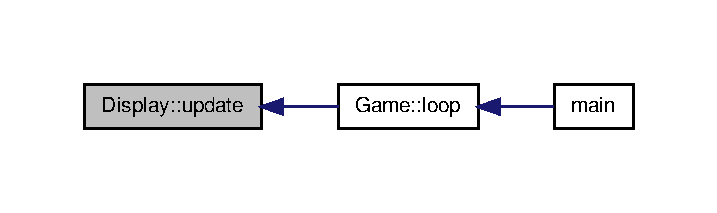
\includegraphics[width=344pt]{class_display_a713ee81045f32895c2b063037c81c388_icgraph}
\end{center}
\end{figure}




The documentation for this class was generated from the following files\-:\begin{DoxyCompactItemize}
\item 
src/\hyperlink{display_8h}{display.\-h}\item 
src/\hyperlink{display_8cpp}{display.\-cpp}\end{DoxyCompactItemize}

\hypertarget{class_entity}{\section{Entity Class Reference}
\label{class_entity}\index{Entity@{Entity}}
}


Abstract class represtenting any displayable physical object of the game.  




{\ttfamily \#include $<$entity.\-h$>$}



Inheritance diagram for Entity\-:\nopagebreak
\begin{figure}[H]
\begin{center}
\leavevmode
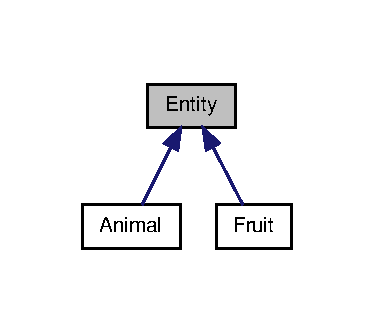
\includegraphics[width=180pt]{class_entity__inherit__graph}
\end{center}
\end{figure}


Collaboration diagram for Entity\-:
\nopagebreak
\begin{figure}[H]
\begin{center}
\leavevmode
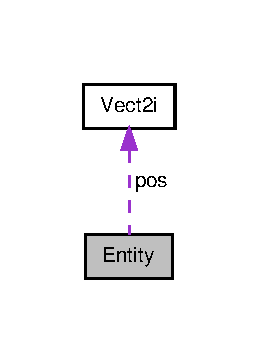
\includegraphics[width=124pt]{class_entity__coll__graph}
\end{center}
\end{figure}
\subsection*{Public Member Functions}
\begin{DoxyCompactItemize}
\item 
\hyperlink{class_entity_a980f368aa07ce358583982821533a54a}{Entity} ()
\item 
virtual \hyperlink{class_entity_a588098978eea6a3486b7361605ff3f0f}{$\sim$\-Entity} ()
\item 
virtual void \hyperlink{class_entity_a31e6183ea44922d54a43be48b8fd4bc0}{init} ()=0
\begin{DoxyCompactList}\small\item\em Abstract method for object initialisation. \end{DoxyCompactList}\item 
\hyperlink{struct_vect2i}{Vect2i} \hyperlink{class_entity_ac010fabbecbd86e008c69560bd216b86}{get\-Pos} () const 
\item 
int \hyperlink{class_entity_ac2f290a20927f548e8742976b222a556}{get\-Radius} () const 
\item 
float \hyperlink{class_entity_a9cecc58b1b2f0c124701ff7add1b8224}{get\-Angle} () const 
\end{DoxyCompactItemize}
\subsection*{Protected Attributes}
\begin{DoxyCompactItemize}
\item 
\hyperlink{struct_vect2i}{Vect2i} \hyperlink{class_entity_a885ee23e7a2132f0d890bb2e312e6d77}{pos}
\item 
float \hyperlink{class_entity_abb6791bd923767cdf42a7e3101a6f76d}{angle}
\item 
int \hyperlink{class_entity_acd7af12063926ab8cd654539328e5532}{radius}
\item 
const int \hyperlink{class_entity_a2b870ef127d06e3f98109695817a1798}{W\-O\-R\-L\-D\-\_\-\-S\-I\-Z\-E}
\end{DoxyCompactItemize}


\subsection{Detailed Description}
Abstract class represtenting any displayable physical object of the game. 

Definition at line 10 of file entity.\-h.



\subsection{Constructor \& Destructor Documentation}
\hypertarget{class_entity_a980f368aa07ce358583982821533a54a}{\index{Entity@{Entity}!Entity@{Entity}}
\index{Entity@{Entity}!Entity@{Entity}}
\subsubsection[{Entity}]{\setlength{\rightskip}{0pt plus 5cm}Entity\-::\-Entity (
\begin{DoxyParamCaption}
{}
\end{DoxyParamCaption}
)}}\label{class_entity_a980f368aa07ce358583982821533a54a}


Definition at line 3 of file entity.\-cpp.

\hypertarget{class_entity_a588098978eea6a3486b7361605ff3f0f}{\index{Entity@{Entity}!$\sim$\-Entity@{$\sim$\-Entity}}
\index{$\sim$\-Entity@{$\sim$\-Entity}!Entity@{Entity}}
\subsubsection[{$\sim$\-Entity}]{\setlength{\rightskip}{0pt plus 5cm}virtual Entity\-::$\sim$\-Entity (
\begin{DoxyParamCaption}
{}
\end{DoxyParamCaption}
)\hspace{0.3cm}{\ttfamily [inline]}, {\ttfamily [virtual]}}}\label{class_entity_a588098978eea6a3486b7361605ff3f0f}


Definition at line 13 of file entity.\-h.



\subsection{Member Function Documentation}
\hypertarget{class_entity_a9cecc58b1b2f0c124701ff7add1b8224}{\index{Entity@{Entity}!get\-Angle@{get\-Angle}}
\index{get\-Angle@{get\-Angle}!Entity@{Entity}}
\subsubsection[{get\-Angle}]{\setlength{\rightskip}{0pt plus 5cm}float Entity\-::get\-Angle (
\begin{DoxyParamCaption}
{}
\end{DoxyParamCaption}
) const\hspace{0.3cm}{\ttfamily [inline]}}}\label{class_entity_a9cecc58b1b2f0c124701ff7add1b8224}


Definition at line 23 of file entity.\-h.

\hypertarget{class_entity_ac010fabbecbd86e008c69560bd216b86}{\index{Entity@{Entity}!get\-Pos@{get\-Pos}}
\index{get\-Pos@{get\-Pos}!Entity@{Entity}}
\subsubsection[{get\-Pos}]{\setlength{\rightskip}{0pt plus 5cm}{\bf Vect2i} Entity\-::get\-Pos (
\begin{DoxyParamCaption}
{}
\end{DoxyParamCaption}
) const\hspace{0.3cm}{\ttfamily [inline]}}}\label{class_entity_ac010fabbecbd86e008c69560bd216b86}


Definition at line 21 of file entity.\-h.

\hypertarget{class_entity_ac2f290a20927f548e8742976b222a556}{\index{Entity@{Entity}!get\-Radius@{get\-Radius}}
\index{get\-Radius@{get\-Radius}!Entity@{Entity}}
\subsubsection[{get\-Radius}]{\setlength{\rightskip}{0pt plus 5cm}int Entity\-::get\-Radius (
\begin{DoxyParamCaption}
{}
\end{DoxyParamCaption}
) const\hspace{0.3cm}{\ttfamily [inline]}}}\label{class_entity_ac2f290a20927f548e8742976b222a556}


Definition at line 22 of file entity.\-h.

\hypertarget{class_entity_a31e6183ea44922d54a43be48b8fd4bc0}{\index{Entity@{Entity}!init@{init}}
\index{init@{init}!Entity@{Entity}}
\subsubsection[{init}]{\setlength{\rightskip}{0pt plus 5cm}virtual void Entity\-::init (
\begin{DoxyParamCaption}
{}
\end{DoxyParamCaption}
)\hspace{0.3cm}{\ttfamily [pure virtual]}}}\label{class_entity_a31e6183ea44922d54a43be48b8fd4bc0}


Abstract method for object initialisation. 



Implemented in \hyperlink{class_fruit_a6a7c7d5b678582f6e941e7f78e5fba2e}{Fruit}, and \hyperlink{class_animal_acd693bbac16d2f7dec930124887a9095}{Animal}.



\subsection{Member Data Documentation}
\hypertarget{class_entity_abb6791bd923767cdf42a7e3101a6f76d}{\index{Entity@{Entity}!angle@{angle}}
\index{angle@{angle}!Entity@{Entity}}
\subsubsection[{angle}]{\setlength{\rightskip}{0pt plus 5cm}float Entity\-::angle\hspace{0.3cm}{\ttfamily [protected]}}}\label{class_entity_abb6791bd923767cdf42a7e3101a6f76d}


Definition at line 27 of file entity.\-h.

\hypertarget{class_entity_a885ee23e7a2132f0d890bb2e312e6d77}{\index{Entity@{Entity}!pos@{pos}}
\index{pos@{pos}!Entity@{Entity}}
\subsubsection[{pos}]{\setlength{\rightskip}{0pt plus 5cm}{\bf Vect2i} Entity\-::pos\hspace{0.3cm}{\ttfamily [protected]}}}\label{class_entity_a885ee23e7a2132f0d890bb2e312e6d77}


Definition at line 26 of file entity.\-h.

\hypertarget{class_entity_acd7af12063926ab8cd654539328e5532}{\index{Entity@{Entity}!radius@{radius}}
\index{radius@{radius}!Entity@{Entity}}
\subsubsection[{radius}]{\setlength{\rightskip}{0pt plus 5cm}int Entity\-::radius\hspace{0.3cm}{\ttfamily [protected]}}}\label{class_entity_acd7af12063926ab8cd654539328e5532}


Definition at line 28 of file entity.\-h.

\hypertarget{class_entity_a2b870ef127d06e3f98109695817a1798}{\index{Entity@{Entity}!W\-O\-R\-L\-D\-\_\-\-S\-I\-Z\-E@{W\-O\-R\-L\-D\-\_\-\-S\-I\-Z\-E}}
\index{W\-O\-R\-L\-D\-\_\-\-S\-I\-Z\-E@{W\-O\-R\-L\-D\-\_\-\-S\-I\-Z\-E}!Entity@{Entity}}
\subsubsection[{W\-O\-R\-L\-D\-\_\-\-S\-I\-Z\-E}]{\setlength{\rightskip}{0pt plus 5cm}const int Entity\-::\-W\-O\-R\-L\-D\-\_\-\-S\-I\-Z\-E\hspace{0.3cm}{\ttfamily [protected]}}}\label{class_entity_a2b870ef127d06e3f98109695817a1798}


Definition at line 30 of file entity.\-h.



The documentation for this class was generated from the following files\-:\begin{DoxyCompactItemize}
\item 
src/\hyperlink{entity_8h}{entity.\-h}\item 
src/\hyperlink{entity_8cpp}{entity.\-cpp}\end{DoxyCompactItemize}

\hypertarget{class_entity_manager}{\section{Entity\-Manager Class Reference}
\label{class_entity_manager}\index{Entity\-Manager@{Entity\-Manager}}
}


Handles the entities, their relations, updates, and all the game mecanics.  




{\ttfamily \#include $<$entity\-\_\-manager.\-h$>$}

\subsection*{Public Member Functions}
\begin{DoxyCompactItemize}
\item 
\hyperlink{class_entity_manager_a7555637657d090171be6ceee8451de0a}{Entity\-Manager} ()
\item 
\hyperlink{class_entity_manager_a71a36c9fb8d579a1a1ec108e0fccf175}{$\sim$\-Entity\-Manager} ()
\item 
void \hyperlink{class_entity_manager_ae0abecb1a8037d6af51d950491115bfb}{init} ()
\begin{DoxyCompactList}\small\item\em Initialise game elements for a new generation. \end{DoxyCompactList}\item 
void \hyperlink{class_entity_manager_abc6a2cc5077501f4b06d88f4ed3e7e31}{update} ()
\begin{DoxyCompactList}\small\item\em Update the game elements. \end{DoxyCompactList}\item 
std\-::vector$<$ \hyperlink{struct_species}{Species} $>$ \hyperlink{class_entity_manager_ac6f76079b0963ac7386a79b6bd346bd8}{get\-Species} () const 
\item 
std\-::vector$<$ \hyperlink{class_fruit}{Fruit} $\ast$ $>$ \hyperlink{class_entity_manager_aa54e413de0914b0f7e048627b7dc07f4}{get\-Fruits} () const 
\end{DoxyCompactItemize}


\subsection{Detailed Description}
Handles the entities, their relations, updates, and all the game mecanics. 

Definition at line 24 of file entity\-\_\-manager.\-h.



\subsection{Constructor \& Destructor Documentation}
\hypertarget{class_entity_manager_a7555637657d090171be6ceee8451de0a}{\index{Entity\-Manager@{Entity\-Manager}!Entity\-Manager@{Entity\-Manager}}
\index{Entity\-Manager@{Entity\-Manager}!EntityManager@{Entity\-Manager}}
\subsubsection[{Entity\-Manager}]{\setlength{\rightskip}{0pt plus 5cm}Entity\-Manager\-::\-Entity\-Manager (
\begin{DoxyParamCaption}
{}
\end{DoxyParamCaption}
)}}\label{class_entity_manager_a7555637657d090171be6ceee8451de0a}


Definition at line 4 of file entity\-\_\-manager.\-cpp.



Here is the call graph for this function\-:
\nopagebreak
\begin{figure}[H]
\begin{center}
\leavevmode
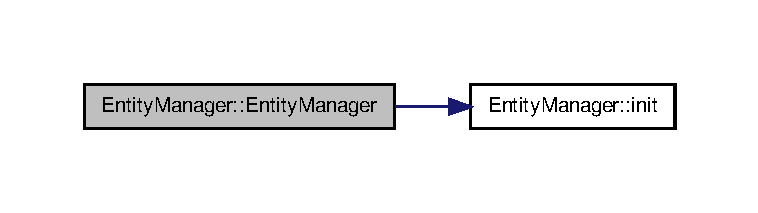
\includegraphics[width=350pt]{class_entity_manager_a7555637657d090171be6ceee8451de0a_cgraph}
\end{center}
\end{figure}


\hypertarget{class_entity_manager_a71a36c9fb8d579a1a1ec108e0fccf175}{\index{Entity\-Manager@{Entity\-Manager}!$\sim$\-Entity\-Manager@{$\sim$\-Entity\-Manager}}
\index{$\sim$\-Entity\-Manager@{$\sim$\-Entity\-Manager}!EntityManager@{Entity\-Manager}}
\subsubsection[{$\sim$\-Entity\-Manager}]{\setlength{\rightskip}{0pt plus 5cm}Entity\-Manager\-::$\sim$\-Entity\-Manager (
\begin{DoxyParamCaption}
{}
\end{DoxyParamCaption}
)}}\label{class_entity_manager_a71a36c9fb8d579a1a1ec108e0fccf175}


Definition at line 36 of file entity\-\_\-manager.\-cpp.



\subsection{Member Function Documentation}
\hypertarget{class_entity_manager_aa54e413de0914b0f7e048627b7dc07f4}{\index{Entity\-Manager@{Entity\-Manager}!get\-Fruits@{get\-Fruits}}
\index{get\-Fruits@{get\-Fruits}!EntityManager@{Entity\-Manager}}
\subsubsection[{get\-Fruits}]{\setlength{\rightskip}{0pt plus 5cm}std\-::vector$<${\bf Fruit}$\ast$$>$ Entity\-Manager\-::get\-Fruits (
\begin{DoxyParamCaption}
{}
\end{DoxyParamCaption}
) const\hspace{0.3cm}{\ttfamily [inline]}}}\label{class_entity_manager_aa54e413de0914b0f7e048627b7dc07f4}


Definition at line 41 of file entity\-\_\-manager.\-h.

\hypertarget{class_entity_manager_ac6f76079b0963ac7386a79b6bd346bd8}{\index{Entity\-Manager@{Entity\-Manager}!get\-Species@{get\-Species}}
\index{get\-Species@{get\-Species}!EntityManager@{Entity\-Manager}}
\subsubsection[{get\-Species}]{\setlength{\rightskip}{0pt plus 5cm}std\-::vector$<${\bf Species}$>$ Entity\-Manager\-::get\-Species (
\begin{DoxyParamCaption}
{}
\end{DoxyParamCaption}
) const\hspace{0.3cm}{\ttfamily [inline]}}}\label{class_entity_manager_ac6f76079b0963ac7386a79b6bd346bd8}


Definition at line 40 of file entity\-\_\-manager.\-h.



Here is the caller graph for this function\-:
\nopagebreak
\begin{figure}[H]
\begin{center}
\leavevmode
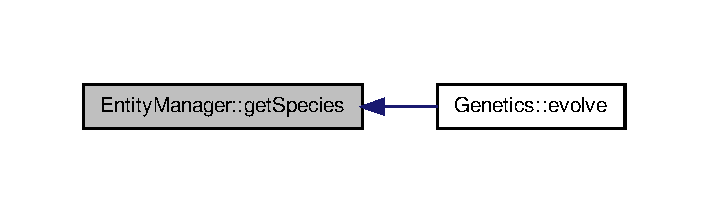
\includegraphics[width=340pt]{class_entity_manager_ac6f76079b0963ac7386a79b6bd346bd8_icgraph}
\end{center}
\end{figure}


\hypertarget{class_entity_manager_ae0abecb1a8037d6af51d950491115bfb}{\index{Entity\-Manager@{Entity\-Manager}!init@{init}}
\index{init@{init}!EntityManager@{Entity\-Manager}}
\subsubsection[{init}]{\setlength{\rightskip}{0pt plus 5cm}void Entity\-Manager\-::init (
\begin{DoxyParamCaption}
{}
\end{DoxyParamCaption}
)}}\label{class_entity_manager_ae0abecb1a8037d6af51d950491115bfb}


Initialise game elements for a new generation. 



Definition at line 52 of file entity\-\_\-manager.\-cpp.



Here is the caller graph for this function\-:
\nopagebreak
\begin{figure}[H]
\begin{center}
\leavevmode
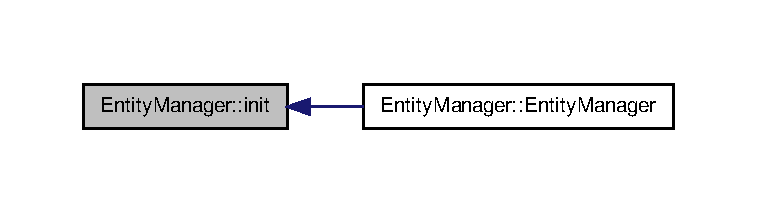
\includegraphics[width=350pt]{class_entity_manager_ae0abecb1a8037d6af51d950491115bfb_icgraph}
\end{center}
\end{figure}


\hypertarget{class_entity_manager_abc6a2cc5077501f4b06d88f4ed3e7e31}{\index{Entity\-Manager@{Entity\-Manager}!update@{update}}
\index{update@{update}!EntityManager@{Entity\-Manager}}
\subsubsection[{update}]{\setlength{\rightskip}{0pt plus 5cm}void Entity\-Manager\-::update (
\begin{DoxyParamCaption}
{}
\end{DoxyParamCaption}
)}}\label{class_entity_manager_abc6a2cc5077501f4b06d88f4ed3e7e31}


Update the game elements. 



Definition at line 70 of file entity\-\_\-manager.\-cpp.



Here is the call graph for this function\-:
\nopagebreak
\begin{figure}[H]
\begin{center}
\leavevmode
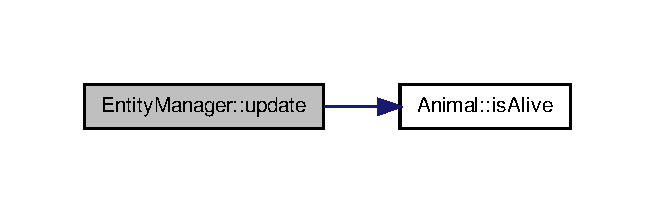
\includegraphics[width=314pt]{class_entity_manager_abc6a2cc5077501f4b06d88f4ed3e7e31_cgraph}
\end{center}
\end{figure}




The documentation for this class was generated from the following files\-:\begin{DoxyCompactItemize}
\item 
src/\hyperlink{entity__manager_8h}{entity\-\_\-manager.\-h}\item 
src/\hyperlink{entity__manager_8cpp}{entity\-\_\-manager.\-cpp}\end{DoxyCompactItemize}

\hypertarget{class_fruit}{\section{Fruit Class Reference}
\label{class_fruit}\index{Fruit@{Fruit}}
}


class representing a fruit \-: static element that can be eaten by an animal  




{\ttfamily \#include $<$fruit.\-h$>$}



Inheritance diagram for Fruit\-:
\nopagebreak
\begin{figure}[H]
\begin{center}
\leavevmode
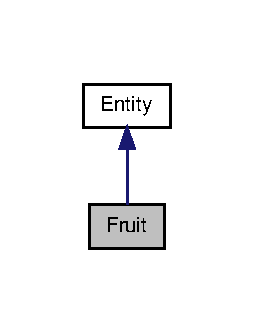
\includegraphics[width=122pt]{class_fruit__inherit__graph}
\end{center}
\end{figure}


Collaboration diagram for Fruit\-:
\nopagebreak
\begin{figure}[H]
\begin{center}
\leavevmode
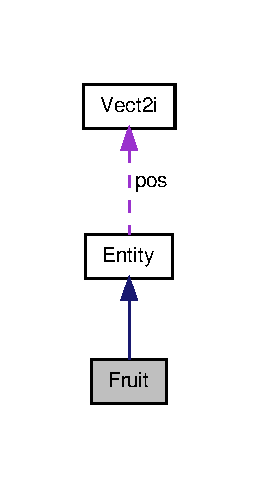
\includegraphics[width=124pt]{class_fruit__coll__graph}
\end{center}
\end{figure}
\subsection*{Public Member Functions}
\begin{DoxyCompactItemize}
\item 
\hyperlink{class_fruit_aa40ce1fdb1b361880d27171f05a2ab5a}{Fruit} ()
\item 
virtual \hyperlink{class_fruit_abd3325dd4faef5b64785aa61cd4046fa}{$\sim$\-Fruit} ()
\item 
virtual void \hyperlink{class_fruit_a6a7c7d5b678582f6e941e7f78e5fba2e}{init} ()
\begin{DoxyCompactList}\small\item\em Abstract method for object initialisation. \end{DoxyCompactList}\item 
void \hyperlink{class_fruit_a231aadb8a3dbf6fe68fc36a0435ff15b}{init} (const \hyperlink{struct_bush}{Bush} \&bush)
\begin{DoxyCompactList}\small\item\em Initialise a fruit somewhere near the bush in parameter. \end{DoxyCompactList}\end{DoxyCompactItemize}
\subsection*{Additional Inherited Members}


\subsection{Detailed Description}
class representing a fruit \-: static element that can be eaten by an animal 

Definition at line 18 of file fruit.\-h.



\subsection{Constructor \& Destructor Documentation}
\hypertarget{class_fruit_aa40ce1fdb1b361880d27171f05a2ab5a}{\index{Fruit@{Fruit}!Fruit@{Fruit}}
\index{Fruit@{Fruit}!Fruit@{Fruit}}
\subsubsection[{Fruit}]{\setlength{\rightskip}{0pt plus 5cm}Fruit\-::\-Fruit (
\begin{DoxyParamCaption}
{}
\end{DoxyParamCaption}
)}}\label{class_fruit_aa40ce1fdb1b361880d27171f05a2ab5a}


Definition at line 3 of file fruit.\-cpp.



Here is the call graph for this function\-:
\nopagebreak
\begin{figure}[H]
\begin{center}
\leavevmode
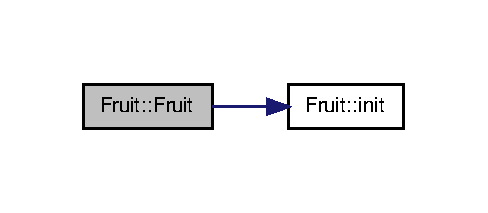
\includegraphics[width=234pt]{class_fruit_aa40ce1fdb1b361880d27171f05a2ab5a_cgraph}
\end{center}
\end{figure}


\hypertarget{class_fruit_abd3325dd4faef5b64785aa61cd4046fa}{\index{Fruit@{Fruit}!$\sim$\-Fruit@{$\sim$\-Fruit}}
\index{$\sim$\-Fruit@{$\sim$\-Fruit}!Fruit@{Fruit}}
\subsubsection[{$\sim$\-Fruit}]{\setlength{\rightskip}{0pt plus 5cm}virtual Fruit\-::$\sim$\-Fruit (
\begin{DoxyParamCaption}
{}
\end{DoxyParamCaption}
)\hspace{0.3cm}{\ttfamily [inline]}, {\ttfamily [virtual]}}}\label{class_fruit_abd3325dd4faef5b64785aa61cd4046fa}


Definition at line 21 of file fruit.\-h.



\subsection{Member Function Documentation}
\hypertarget{class_fruit_a6a7c7d5b678582f6e941e7f78e5fba2e}{\index{Fruit@{Fruit}!init@{init}}
\index{init@{init}!Fruit@{Fruit}}
\subsubsection[{init}]{\setlength{\rightskip}{0pt plus 5cm}void Fruit\-::init (
\begin{DoxyParamCaption}
{}
\end{DoxyParamCaption}
)\hspace{0.3cm}{\ttfamily [virtual]}}}\label{class_fruit_a6a7c7d5b678582f6e941e7f78e5fba2e}


Abstract method for object initialisation. 



Implements \hyperlink{class_entity_a31e6183ea44922d54a43be48b8fd4bc0}{Entity}.



Definition at line 9 of file fruit.\-cpp.



Here is the caller graph for this function\-:
\nopagebreak
\begin{figure}[H]
\begin{center}
\leavevmode
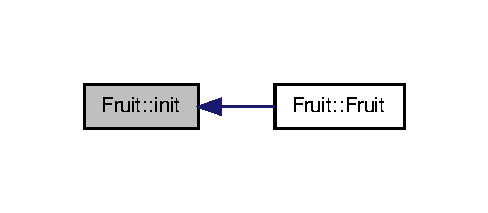
\includegraphics[width=234pt]{class_fruit_a6a7c7d5b678582f6e941e7f78e5fba2e_icgraph}
\end{center}
\end{figure}


\hypertarget{class_fruit_a231aadb8a3dbf6fe68fc36a0435ff15b}{\index{Fruit@{Fruit}!init@{init}}
\index{init@{init}!Fruit@{Fruit}}
\subsubsection[{init}]{\setlength{\rightskip}{0pt plus 5cm}void Fruit\-::init (
\begin{DoxyParamCaption}
\item[{const {\bf Bush} \&}]{bush}
\end{DoxyParamCaption}
)}}\label{class_fruit_a231aadb8a3dbf6fe68fc36a0435ff15b}


Initialise a fruit somewhere near the bush in parameter. 


\begin{DoxyParams}{Parameters}
{\em bush} & The bush the fruit belongs to \\
\hline
\end{DoxyParams}


Definition at line 14 of file fruit.\-cpp.



The documentation for this class was generated from the following files\-:\begin{DoxyCompactItemize}
\item 
src/\hyperlink{fruit_8h}{fruit.\-h}\item 
src/\hyperlink{fruit_8cpp}{fruit.\-cpp}\end{DoxyCompactItemize}

\hypertarget{class_game}{\section{Game Class Reference}
\label{class_game}\index{Game@{Game}}
}


General class dispatching the game jobs to other objects. Only S\-F\-M\-L user with \hyperlink{class_display}{Display}.  




{\ttfamily \#include $<$game.\-h$>$}

\subsection*{Public Member Functions}
\begin{DoxyCompactItemize}
\item 
\hyperlink{class_game_ad59df6562a58a614fda24622d3715b65}{Game} ()
\item 
\hyperlink{class_game_ae3d112ca6e0e55150d2fdbc704474530}{$\sim$\-Game} ()
\item 
void \hyperlink{class_game_a7ad92b77b596d7882a7ae76eb18b5e6c}{loop} ()
\begin{DoxyCompactList}\small\item\em \hyperlink{class_game}{Game} loop. \end{DoxyCompactList}\item 
void \hyperlink{class_game_a8272be134d16c277bb014ad6a22fc357}{quit} ()
\item 
void \hyperlink{class_game_a7c89563d299f25881c8c8a42c1e3219e}{increase\-Game\-Speed} ()
\item 
void \hyperlink{class_game_adcf5df2f7a3f5209f974741667b1236f}{decrease\-Game\-Speed} ()
\item 
int \hyperlink{class_game_a3949b192e3277375cd07c98d3360bc44}{get\-Generation} () const 
\item 
int \hyperlink{class_game_adc07928f26c664cefc2c6abee7846d5e}{get\-Iterations} () const 
\item 
int \hyperlink{class_game_abcda9001eb350576bae25bc51b567422}{get\-Iterations\-Per\-Generation} () const 
\item 
float \hyperlink{class_game_a16dc509013f9a07a905656830bfa674d}{get\-Game\-Speed\-Ratio} () const 
\item 
float \hyperlink{class_game_a90335116dc7ad193f6476a0c2a502662}{get\-Fps} () const 
\item 
float \hyperlink{class_game_aa555c6e4a6d743384a99c55d75a37bd2}{get\-Ups} () const 
\end{DoxyCompactItemize}


\subsection{Detailed Description}
General class dispatching the game jobs to other objects. Only S\-F\-M\-L user with \hyperlink{class_display}{Display}. 

Definition at line 20 of file game.\-h.



\subsection{Constructor \& Destructor Documentation}
\hypertarget{class_game_ad59df6562a58a614fda24622d3715b65}{\index{Game@{Game}!Game@{Game}}
\index{Game@{Game}!Game@{Game}}
\subsubsection[{Game}]{\setlength{\rightskip}{0pt plus 5cm}Game\-::\-Game (
\begin{DoxyParamCaption}
{}
\end{DoxyParamCaption}
)}}\label{class_game_ad59df6562a58a614fda24622d3715b65}


Definition at line 4 of file game.\-cpp.

\hypertarget{class_game_ae3d112ca6e0e55150d2fdbc704474530}{\index{Game@{Game}!$\sim$\-Game@{$\sim$\-Game}}
\index{$\sim$\-Game@{$\sim$\-Game}!Game@{Game}}
\subsubsection[{$\sim$\-Game}]{\setlength{\rightskip}{0pt plus 5cm}Game\-::$\sim$\-Game (
\begin{DoxyParamCaption}
{}
\end{DoxyParamCaption}
)}}\label{class_game_ae3d112ca6e0e55150d2fdbc704474530}


Definition at line 12 of file game.\-cpp.



\subsection{Member Function Documentation}
\hypertarget{class_game_adcf5df2f7a3f5209f974741667b1236f}{\index{Game@{Game}!decrease\-Game\-Speed@{decrease\-Game\-Speed}}
\index{decrease\-Game\-Speed@{decrease\-Game\-Speed}!Game@{Game}}
\subsubsection[{decrease\-Game\-Speed}]{\setlength{\rightskip}{0pt plus 5cm}void Game\-::decrease\-Game\-Speed (
\begin{DoxyParamCaption}
{}
\end{DoxyParamCaption}
)}}\label{class_game_adcf5df2f7a3f5209f974741667b1236f}


Definition at line 49 of file game.\-cpp.



Here is the caller graph for this function\-:\nopagebreak
\begin{figure}[H]
\begin{center}
\leavevmode
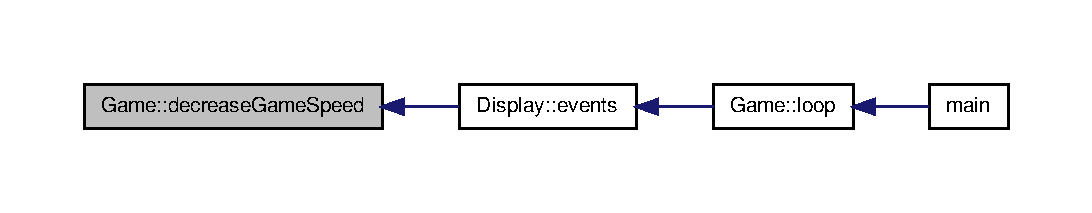
\includegraphics[width=350pt]{class_game_adcf5df2f7a3f5209f974741667b1236f_icgraph}
\end{center}
\end{figure}


\hypertarget{class_game_a90335116dc7ad193f6476a0c2a502662}{\index{Game@{Game}!get\-Fps@{get\-Fps}}
\index{get\-Fps@{get\-Fps}!Game@{Game}}
\subsubsection[{get\-Fps}]{\setlength{\rightskip}{0pt plus 5cm}float Game\-::get\-Fps (
\begin{DoxyParamCaption}
{}
\end{DoxyParamCaption}
) const\hspace{0.3cm}{\ttfamily [inline]}}}\label{class_game_a90335116dc7ad193f6476a0c2a502662}


Definition at line 39 of file game.\-h.

\hypertarget{class_game_a16dc509013f9a07a905656830bfa674d}{\index{Game@{Game}!get\-Game\-Speed\-Ratio@{get\-Game\-Speed\-Ratio}}
\index{get\-Game\-Speed\-Ratio@{get\-Game\-Speed\-Ratio}!Game@{Game}}
\subsubsection[{get\-Game\-Speed\-Ratio}]{\setlength{\rightskip}{0pt plus 5cm}float Game\-::get\-Game\-Speed\-Ratio (
\begin{DoxyParamCaption}
{}
\end{DoxyParamCaption}
) const\hspace{0.3cm}{\ttfamily [inline]}}}\label{class_game_a16dc509013f9a07a905656830bfa674d}


Definition at line 38 of file game.\-h.

\hypertarget{class_game_a3949b192e3277375cd07c98d3360bc44}{\index{Game@{Game}!get\-Generation@{get\-Generation}}
\index{get\-Generation@{get\-Generation}!Game@{Game}}
\subsubsection[{get\-Generation}]{\setlength{\rightskip}{0pt plus 5cm}int Game\-::get\-Generation (
\begin{DoxyParamCaption}
{}
\end{DoxyParamCaption}
) const\hspace{0.3cm}{\ttfamily [inline]}}}\label{class_game_a3949b192e3277375cd07c98d3360bc44}


Definition at line 35 of file game.\-h.

\hypertarget{class_game_adc07928f26c664cefc2c6abee7846d5e}{\index{Game@{Game}!get\-Iterations@{get\-Iterations}}
\index{get\-Iterations@{get\-Iterations}!Game@{Game}}
\subsubsection[{get\-Iterations}]{\setlength{\rightskip}{0pt plus 5cm}int Game\-::get\-Iterations (
\begin{DoxyParamCaption}
{}
\end{DoxyParamCaption}
) const\hspace{0.3cm}{\ttfamily [inline]}}}\label{class_game_adc07928f26c664cefc2c6abee7846d5e}


Definition at line 36 of file game.\-h.

\hypertarget{class_game_abcda9001eb350576bae25bc51b567422}{\index{Game@{Game}!get\-Iterations\-Per\-Generation@{get\-Iterations\-Per\-Generation}}
\index{get\-Iterations\-Per\-Generation@{get\-Iterations\-Per\-Generation}!Game@{Game}}
\subsubsection[{get\-Iterations\-Per\-Generation}]{\setlength{\rightskip}{0pt plus 5cm}int Game\-::get\-Iterations\-Per\-Generation (
\begin{DoxyParamCaption}
{}
\end{DoxyParamCaption}
) const\hspace{0.3cm}{\ttfamily [inline]}}}\label{class_game_abcda9001eb350576bae25bc51b567422}


Definition at line 37 of file game.\-h.

\hypertarget{class_game_aa555c6e4a6d743384a99c55d75a37bd2}{\index{Game@{Game}!get\-Ups@{get\-Ups}}
\index{get\-Ups@{get\-Ups}!Game@{Game}}
\subsubsection[{get\-Ups}]{\setlength{\rightskip}{0pt plus 5cm}float Game\-::get\-Ups (
\begin{DoxyParamCaption}
{}
\end{DoxyParamCaption}
) const\hspace{0.3cm}{\ttfamily [inline]}}}\label{class_game_aa555c6e4a6d743384a99c55d75a37bd2}


Definition at line 40 of file game.\-h.

\hypertarget{class_game_a7c89563d299f25881c8c8a42c1e3219e}{\index{Game@{Game}!increase\-Game\-Speed@{increase\-Game\-Speed}}
\index{increase\-Game\-Speed@{increase\-Game\-Speed}!Game@{Game}}
\subsubsection[{increase\-Game\-Speed}]{\setlength{\rightskip}{0pt plus 5cm}void Game\-::increase\-Game\-Speed (
\begin{DoxyParamCaption}
{}
\end{DoxyParamCaption}
)}}\label{class_game_a7c89563d299f25881c8c8a42c1e3219e}


Definition at line 46 of file game.\-cpp.



Here is the caller graph for this function\-:\nopagebreak
\begin{figure}[H]
\begin{center}
\leavevmode
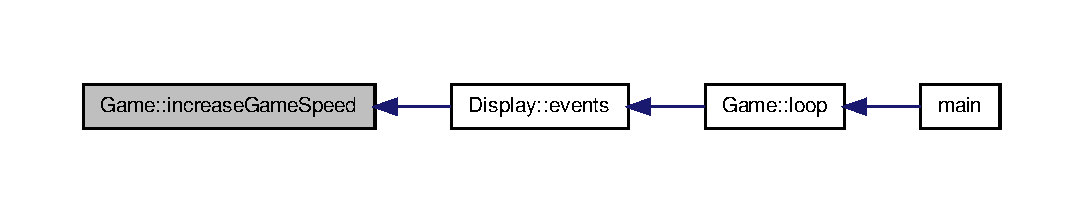
\includegraphics[width=350pt]{class_game_a7c89563d299f25881c8c8a42c1e3219e_icgraph}
\end{center}
\end{figure}


\hypertarget{class_game_a7ad92b77b596d7882a7ae76eb18b5e6c}{\index{Game@{Game}!loop@{loop}}
\index{loop@{loop}!Game@{Game}}
\subsubsection[{loop}]{\setlength{\rightskip}{0pt plus 5cm}void Game\-::loop (
\begin{DoxyParamCaption}
{}
\end{DoxyParamCaption}
)}}\label{class_game_a7ad92b77b596d7882a7ae76eb18b5e6c}


\hyperlink{class_game}{Game} loop. 



Definition at line 19 of file game.\-cpp.



Here is the call graph for this function\-:\nopagebreak
\begin{figure}[H]
\begin{center}
\leavevmode
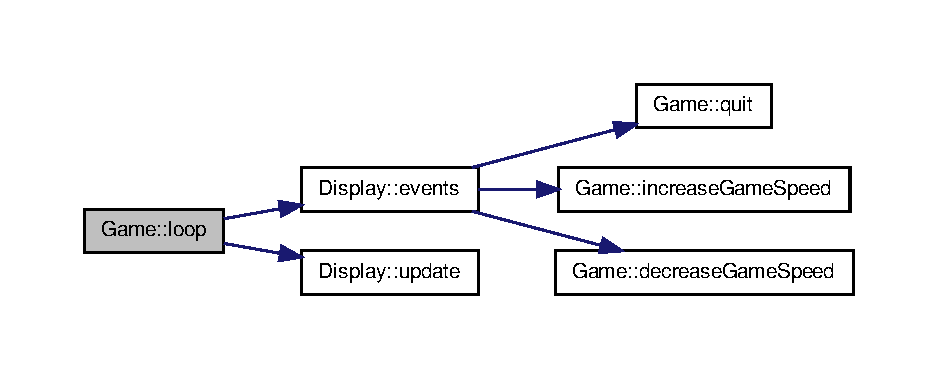
\includegraphics[width=350pt]{class_game_a7ad92b77b596d7882a7ae76eb18b5e6c_cgraph}
\end{center}
\end{figure}




Here is the caller graph for this function\-:\nopagebreak
\begin{figure}[H]
\begin{center}
\leavevmode
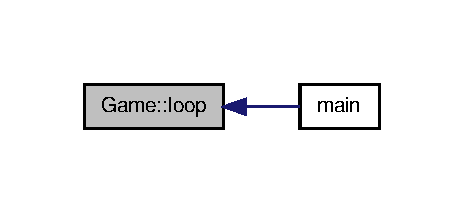
\includegraphics[width=222pt]{class_game_a7ad92b77b596d7882a7ae76eb18b5e6c_icgraph}
\end{center}
\end{figure}


\hypertarget{class_game_a8272be134d16c277bb014ad6a22fc357}{\index{Game@{Game}!quit@{quit}}
\index{quit@{quit}!Game@{Game}}
\subsubsection[{quit}]{\setlength{\rightskip}{0pt plus 5cm}void Game\-::quit (
\begin{DoxyParamCaption}
{}
\end{DoxyParamCaption}
)\hspace{0.3cm}{\ttfamily [inline]}}}\label{class_game_a8272be134d16c277bb014ad6a22fc357}


Definition at line 30 of file game.\-h.



Here is the caller graph for this function\-:\nopagebreak
\begin{figure}[H]
\begin{center}
\leavevmode
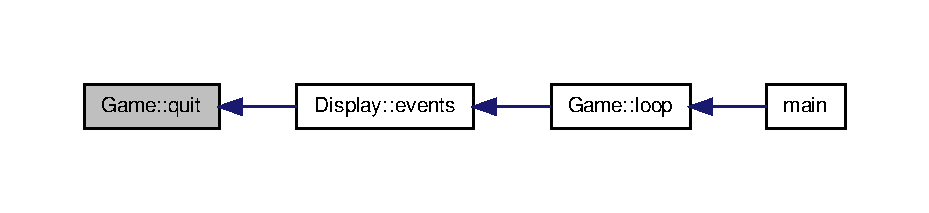
\includegraphics[width=350pt]{class_game_a8272be134d16c277bb014ad6a22fc357_icgraph}
\end{center}
\end{figure}




The documentation for this class was generated from the following files\-:\begin{DoxyCompactItemize}
\item 
src/\hyperlink{game_8h}{game.\-h}\item 
src/\hyperlink{game_8cpp}{game.\-cpp}\end{DoxyCompactItemize}

\hypertarget{class_genetics}{\section{Genetics Class Reference}
\label{class_genetics}\index{Genetics@{Genetics}}
}


More or less static class operating the genetic algorithm on all the animal species of the \hyperlink{class_entity_manager}{Entity\-Manager}.  




{\ttfamily \#include $<$genetics.\-h$>$}

\subsection*{Public Member Functions}
\begin{DoxyCompactItemize}
\item 
\hyperlink{class_genetics_a7c9a65ee1c7da6bbb4b35d46d1dcf4fa}{Genetics} ()
\item 
void \hyperlink{class_genetics_a63e33bd3725feb511e19d86e2d07ca3b}{evolve} (\hyperlink{class_entity_manager}{Entity\-Manager} \&manager)
\begin{DoxyCompactList}\small\item\em Entry point of the G\-A. \end{DoxyCompactList}\end{DoxyCompactItemize}


\subsection{Detailed Description}
More or less static class operating the genetic algorithm on all the animal species of the \hyperlink{class_entity_manager}{Entity\-Manager}. 

I am not here to discuss the pros and cons of the different implementations of selection, rossover and mutation, however I have quite a lot to say about it. Fear not, I might (someday) right some things about these (very interesting) subjects. But for that I need D\-A\-T\-A ! My software doesn't provide any at the time, and every conclusion I might have made is only a result of a subjective observation.

Likewise, I won't here explain the internal working of the algorithms I used. You have the code right here, and the web is full of documentation. Googling \char`\"{}rank-\/based selection\char`\"{}, \char`\"{}uniform crossover\char`\"{} and such will teach you everything you need to know. Again, I might right something about all this someday. However, if you have interesting data on the different mutation operators that work fine on real values, I'm interested !

Sidenotes of the day \-:
\begin{DoxyItemize}
\item Mutation deviation should be variable, but how ? 
\end{DoxyItemize}

<<<<<<< HEAD
Definition at line 35 of file genetics.\-h.
=======
Definition at line 30 of file genetics.\-h.
>>>>>>> master



\subsection{Constructor \& Destructor Documentation}
\hypertarget{class_genetics_a7c9a65ee1c7da6bbb4b35d46d1dcf4fa}{\index{Genetics@{Genetics}!Genetics@{Genetics}}
\index{Genetics@{Genetics}!Genetics@{Genetics}}
\subsubsection[{Genetics}]{\setlength{\rightskip}{0pt plus 5cm}Genetics\-::\-Genetics (
\begin{DoxyParamCaption}
{}
\end{DoxyParamCaption}
)}}\label{class_genetics_a7c9a65ee1c7da6bbb4b35d46d1dcf4fa}


Definition at line 3 of file genetics.\-cpp.



\subsection{Member Function Documentation}
\hypertarget{class_genetics_a63e33bd3725feb511e19d86e2d07ca3b}{\index{Genetics@{Genetics}!evolve@{evolve}}
\index{evolve@{evolve}!Genetics@{Genetics}}
\subsubsection[{evolve}]{\setlength{\rightskip}{0pt plus 5cm}void Genetics\-::evolve (
\begin{DoxyParamCaption}
\item[{{\bf Entity\-Manager} \&}]{manager}
\end{DoxyParamCaption}
)}}\label{class_genetics_a63e33bd3725feb511e19d86e2d07ca3b}


Entry point of the G\-A. 


\begin{DoxyParams}{Parameters}
{\em manager} & the \hyperlink{class_entity_manager}{Entity\-Manager} where to find the species to evolve\\
\hline
\end{DoxyParams}
Performs the genetic algorithm on every species of the manager 

Definition at line 7 of file genetics.\-cpp.



<<<<<<< HEAD
Here is the call graph for this function\-:
\nopagebreak
=======
Here is the call graph for this function\-:\nopagebreak
>>>>>>> master
\begin{figure}[H]
\begin{center}
\leavevmode
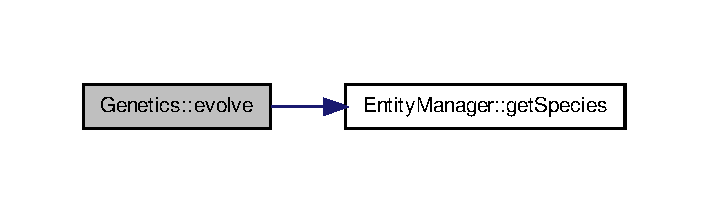
\includegraphics[width=340pt]{class_genetics_a63e33bd3725feb511e19d86e2d07ca3b_cgraph}
\end{center}
\end{figure}




The documentation for this class was generated from the following files\-:\begin{DoxyCompactItemize}
\item 
src/\hyperlink{genetics_8h}{genetics.\-h}\item 
src/\hyperlink{genetics_8cpp}{genetics.\-cpp}\end{DoxyCompactItemize}

\hypertarget{class_layer}{\section{Layer Class Reference}
\label{class_layer}\index{Layer@{Layer}}
}


<<<<<<< HEAD
Class representing a layer of neurons inside the nn.  
=======
Class representing a layer of neurons inside the neural network.  
>>>>>>> master




{\ttfamily \#include $<$layer.\-h$>$}

\subsection*{Public Member Functions}
\begin{DoxyCompactItemize}
\item 
\hyperlink{class_layer_a16d6a7a3cff2e9e489186400a9d0f4f2}{Layer} (unsigned int \-\_\-inputs\-Number, unsigned int \-\_\-neurons\-Number)
\item 
\hyperlink{class_layer_a1b1ba4804451dfe6cc357194e42762ae}{$\sim$\-Layer} ()
\item 
void \hyperlink{class_layer_a08ee50fd54abe23d9fc94551c7b4be3f}{init\-Neurons} ()
\begin{DoxyCompactList}\small\item\em initialize the neurones of the layer with the inputs/outputs numbers \end{DoxyCompactList}\item 
std\-::vector$<$ float $>$ \hyperlink{class_layer_a33387425a6f32b455bdca87496a891c9}{run} (const std\-::vector$<$ float $>$ inputs)
\begin{DoxyCompactList}\small\item\em Execution of all the neurons of the layer according to the inputs array. \end{DoxyCompactList}\item 
std\-::vector$<$ float $>$ \hyperlink{class_layer_a18d9fa45eb9ff61f5d5bb9c74179bf30}{get\-D\-N\-A} ()
\item 
unsigned int \hyperlink{class_layer_a01093e904ef7331b99fccc9abe1174aa}{get\-D\-N\-A\-Size} () const 
\item 
void \hyperlink{class_layer_acd14a68865522c3e63a0dab87dd3a100}{set\-D\-N\-A} (const std\-::vector$<$ float $>$ \&D\-N\-A)
\begin{DoxyCompactList}\small\item\em Update the neurons' D\-N\-A with the news value. \end{DoxyCompactList}\end{DoxyCompactItemize}


\subsection{Detailed Description}
<<<<<<< HEAD
Class representing a layer of neurons inside the nn. 
=======
Class representing a layer of neurons inside the neural network. 
>>>>>>> master


\begin{DoxyParams}{Parameters}
{\em \-\_\-inputs\-Number} & Number of inputs for each neuron \\
\hline
<<<<<<< HEAD
{\em \-\_\-neurons\-Number} & Number of outputs for each neuron \\
\hline
\end{DoxyParams}


Definition at line 16 of file layer.\-h.
=======
{\em \-\_\-neurons\-Number} & Number of outputs for each neuron\\
\hline
\end{DoxyParams}
The wikipedia page of Neural Networks will explain you better what a layer is, so go check out if you have any doubt. \hyperlink{class_neuron}{Neuron} and \hyperlink{class_neural_network}{Neural\-Network} are more interesting classes to investigates, \hyperlink{class_layer}{Layer} is only an intermediate. 

Definition at line 19 of file layer.\-h.
>>>>>>> master



\subsection{Constructor \& Destructor Documentation}
\hypertarget{class_layer_a16d6a7a3cff2e9e489186400a9d0f4f2}{\index{Layer@{Layer}!Layer@{Layer}}
\index{Layer@{Layer}!Layer@{Layer}}
\subsubsection[{Layer}]{\setlength{\rightskip}{0pt plus 5cm}Layer\-::\-Layer (
\begin{DoxyParamCaption}
\item[{unsigned int}]{\-\_\-inputs\-Number, }
\item[{unsigned int}]{\-\_\-neurons\-Number}
\end{DoxyParamCaption}
)}}\label{class_layer_a16d6a7a3cff2e9e489186400a9d0f4f2}


Definition at line 3 of file layer.\-cpp.



<<<<<<< HEAD
Here is the call graph for this function\-:
\nopagebreak
=======
Here is the call graph for this function\-:\nopagebreak
>>>>>>> master
\begin{figure}[H]
\begin{center}
\leavevmode
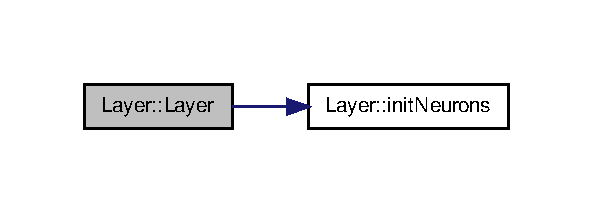
\includegraphics[width=284pt]{class_layer_a16d6a7a3cff2e9e489186400a9d0f4f2_cgraph}
\end{center}
\end{figure}


\hypertarget{class_layer_a1b1ba4804451dfe6cc357194e42762ae}{\index{Layer@{Layer}!$\sim$\-Layer@{$\sim$\-Layer}}
\index{$\sim$\-Layer@{$\sim$\-Layer}!Layer@{Layer}}
\subsubsection[{$\sim$\-Layer}]{\setlength{\rightskip}{0pt plus 5cm}Layer\-::$\sim$\-Layer (
\begin{DoxyParamCaption}
{}
\end{DoxyParamCaption}
)}}\label{class_layer_a1b1ba4804451dfe6cc357194e42762ae}


Definition at line 9 of file layer.\-cpp.



\subsection{Member Function Documentation}
\hypertarget{class_layer_a18d9fa45eb9ff61f5d5bb9c74179bf30}{\index{Layer@{Layer}!get\-D\-N\-A@{get\-D\-N\-A}}
\index{get\-D\-N\-A@{get\-D\-N\-A}!Layer@{Layer}}
\subsubsection[{get\-D\-N\-A}]{\setlength{\rightskip}{0pt plus 5cm}std\-::vector$<$ float $>$ Layer\-::get\-D\-N\-A (
\begin{DoxyParamCaption}
{}
\end{DoxyParamCaption}
)}}\label{class_layer_a18d9fa45eb9ff61f5d5bb9c74179bf30}
\begin{DoxyReturn}{Returns}
the D\-N\-A of all the neurons as a float vector 
\end{DoxyReturn}


Definition at line 32 of file layer.\-cpp.

\hypertarget{class_layer_a01093e904ef7331b99fccc9abe1174aa}{\index{Layer@{Layer}!get\-D\-N\-A\-Size@{get\-D\-N\-A\-Size}}
\index{get\-D\-N\-A\-Size@{get\-D\-N\-A\-Size}!Layer@{Layer}}
\subsubsection[{get\-D\-N\-A\-Size}]{\setlength{\rightskip}{0pt plus 5cm}unsigned int Layer\-::get\-D\-N\-A\-Size (
\begin{DoxyParamCaption}
{}
\end{DoxyParamCaption}
) const}}\label{class_layer_a01093e904ef7331b99fccc9abe1174aa}
\begin{DoxyReturn}{Returns}
<<<<<<< HEAD
The D\-N\-A of all the nuerons size 
=======
The D\-N\-A of all the neurons size 
>>>>>>> master
\end{DoxyReturn}


Definition at line 42 of file layer.\-cpp.

<<<<<<< HEAD
=======


Here is the call graph for this function\-:\nopagebreak
\begin{figure}[H]
\begin{center}
\leavevmode
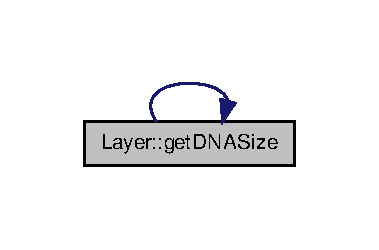
\includegraphics[width=182pt]{class_layer_a01093e904ef7331b99fccc9abe1174aa_cgraph}
\end{center}
\end{figure}




Here is the caller graph for this function\-:\nopagebreak
\begin{figure}[H]
\begin{center}
\leavevmode
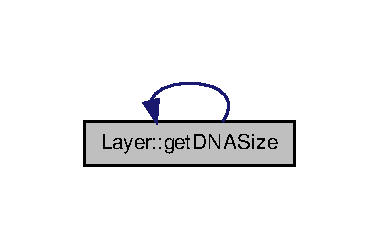
\includegraphics[width=182pt]{class_layer_a01093e904ef7331b99fccc9abe1174aa_icgraph}
\end{center}
\end{figure}


>>>>>>> master
\hypertarget{class_layer_a08ee50fd54abe23d9fc94551c7b4be3f}{\index{Layer@{Layer}!init\-Neurons@{init\-Neurons}}
\index{init\-Neurons@{init\-Neurons}!Layer@{Layer}}
\subsubsection[{init\-Neurons}]{\setlength{\rightskip}{0pt plus 5cm}void Layer\-::init\-Neurons (
\begin{DoxyParamCaption}
{}
\end{DoxyParamCaption}
)}}\label{class_layer_a08ee50fd54abe23d9fc94551c7b4be3f}


initialize the neurones of the layer with the inputs/outputs numbers 



Definition at line 12 of file layer.\-cpp.



<<<<<<< HEAD
Here is the caller graph for this function\-:
\nopagebreak
=======
Here is the caller graph for this function\-:\nopagebreak
>>>>>>> master
\begin{figure}[H]
\begin{center}
\leavevmode
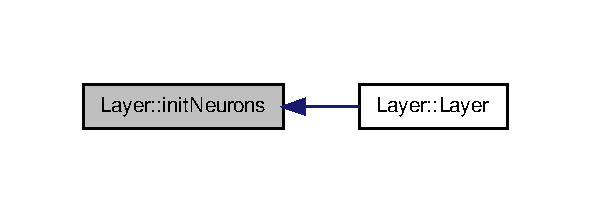
\includegraphics[width=284pt]{class_layer_a08ee50fd54abe23d9fc94551c7b4be3f_icgraph}
\end{center}
\end{figure}


\hypertarget{class_layer_a33387425a6f32b455bdca87496a891c9}{\index{Layer@{Layer}!run@{run}}
\index{run@{run}!Layer@{Layer}}
\subsubsection[{run}]{\setlength{\rightskip}{0pt plus 5cm}std\-::vector$<$ float $>$ Layer\-::run (
\begin{DoxyParamCaption}
\item[{const std\-::vector$<$ float $>$}]{inputs}
\end{DoxyParamCaption}
)}}\label{class_layer_a33387425a6f32b455bdca87496a891c9}


Execution of all the neurons of the layer according to the inputs array. 


\begin{DoxyParams}{Parameters}
{\em inputs} & The inputs array \\
\hline
\end{DoxyParams}
\begin{DoxyReturn}{Returns}
A float array representing the outputs 
\end{DoxyReturn}


Definition at line 23 of file layer.\-cpp.

\hypertarget{class_layer_acd14a68865522c3e63a0dab87dd3a100}{\index{Layer@{Layer}!set\-D\-N\-A@{set\-D\-N\-A}}
\index{set\-D\-N\-A@{set\-D\-N\-A}!Layer@{Layer}}
\subsubsection[{set\-D\-N\-A}]{\setlength{\rightskip}{0pt plus 5cm}void Layer\-::set\-D\-N\-A (
\begin{DoxyParamCaption}
\item[{const std\-::vector$<$ float $>$ \&}]{D\-N\-A}
\end{DoxyParamCaption}
)}}\label{class_layer_acd14a68865522c3e63a0dab87dd3a100}


Update the neurons' D\-N\-A with the news value. 


\begin{DoxyParams}{Parameters}
{\em D\-N\-A} & The new D\-N\-A to set \\
\hline
\end{DoxyParams}


Definition at line 52 of file layer.\-cpp.



The documentation for this class was generated from the following files\-:\begin{DoxyCompactItemize}
\item 
src/\hyperlink{layer_8h}{layer.\-h}\item 
src/\hyperlink{layer_8cpp}{layer.\-cpp}\end{DoxyCompactItemize}

\hypertarget{class_neural_network}{\section{Neural\-Network Class Reference}
\label{class_neural_network}\index{Neural\-Network@{Neural\-Network}}
}


The N\-N class, containing Layers\-Number (form config.\-cfg) layers of neurons, the layers size depending on inputs/ouptus/config.  




{\ttfamily \#include $<$neural\-\_\-network.\-h$>$}

\subsection*{Public Member Functions}
\begin{DoxyCompactItemize}
\item 
\hyperlink{class_neural_network_a3af96ee26597b200166e3a2523d56ad9}{Neural\-Network} (unsigned int \-\_\-inputs\-Number, unsigned int \-\_\-outputs\-Number)
\item 
void \hyperlink{class_neural_network_ace5b58e0174ef1f318db06f0b19f694b}{init\-Layers} ()
\begin{DoxyCompactList}\small\item\em Initialisation of the different layers depending on inputs/outputs/config (for the hidden layer) \end{DoxyCompactList}\item 
std\-::vector$<$ float $>$ \hyperlink{class_neural_network_a2daf940807763cd3d81661f93d99e6ba}{run} (const std\-::vector$<$ float $>$ inputs)
\begin{DoxyCompactList}\small\item\em Runs the calculation of the outputs array depending on the inputs. \end{DoxyCompactList}\item 
std\-::vector$<$ float $>$ \hyperlink{class_neural_network_abd6e6ec0a4500527150c127f0f8d7c23}{get\-D\-N\-A} ()
\item 
void \hyperlink{class_neural_network_a38e8afa4eb8651b80c48b577ecdc6c4a}{set\-D\-N\-A} (const std\-::vector$<$ float $>$ \&D\-N\-A)
\begin{DoxyCompactList}\small\item\em Updates the D\-N\-A of all neurons with the new one, given by the genetics algorithm. \end{DoxyCompactList}\end{DoxyCompactItemize}


\subsection{Detailed Description}
The N\-N class, containing Layers\-Number (form config.\-cfg) layers of neurons, the layers size depending on inputs/ouptus/config. 


\begin{DoxyParams}{Parameters}
{\em \-\_\-inputs\-Number} & The inputs number of the N\-N \\
\hline
{\em \-\_\-outputs\-Number} & The outputs number \\
\hline
\end{DoxyParams}


Definition at line 16 of file neural\-\_\-network.\-h.



\subsection{Constructor \& Destructor Documentation}
\hypertarget{class_neural_network_a3af96ee26597b200166e3a2523d56ad9}{\index{Neural\-Network@{Neural\-Network}!Neural\-Network@{Neural\-Network}}
\index{Neural\-Network@{Neural\-Network}!NeuralNetwork@{Neural\-Network}}
\subsubsection[{Neural\-Network}]{\setlength{\rightskip}{0pt plus 5cm}Neural\-Network\-::\-Neural\-Network (
\begin{DoxyParamCaption}
\item[{unsigned int}]{\-\_\-inputs\-Number, }
\item[{unsigned int}]{\-\_\-outputs\-Number}
\end{DoxyParamCaption}
)}}\label{class_neural_network_a3af96ee26597b200166e3a2523d56ad9}


Definition at line 3 of file neural\-\_\-network.\-cpp.



Here is the call graph for this function\-:
\nopagebreak
\begin{figure}[H]
\begin{center}
\leavevmode
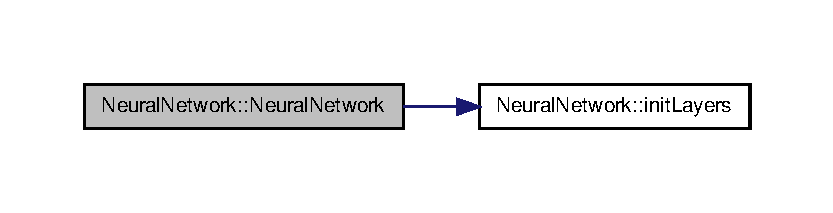
\includegraphics[width=350pt]{class_neural_network_a3af96ee26597b200166e3a2523d56ad9_cgraph}
\end{center}
\end{figure}




\subsection{Member Function Documentation}
\hypertarget{class_neural_network_abd6e6ec0a4500527150c127f0f8d7c23}{\index{Neural\-Network@{Neural\-Network}!get\-D\-N\-A@{get\-D\-N\-A}}
\index{get\-D\-N\-A@{get\-D\-N\-A}!NeuralNetwork@{Neural\-Network}}
\subsubsection[{get\-D\-N\-A}]{\setlength{\rightskip}{0pt plus 5cm}std\-::vector$<$ float $>$ Neural\-Network\-::get\-D\-N\-A (
\begin{DoxyParamCaption}
{}
\end{DoxyParamCaption}
)}}\label{class_neural_network_abd6e6ec0a4500527150c127f0f8d7c23}
\begin{DoxyReturn}{Returns}
The complete D\-N\-A of the N\-N, as an array of float 
\end{DoxyReturn}


Definition at line 43 of file neural\-\_\-network.\-cpp.



Here is the caller graph for this function\-:
\nopagebreak
\begin{figure}[H]
\begin{center}
\leavevmode
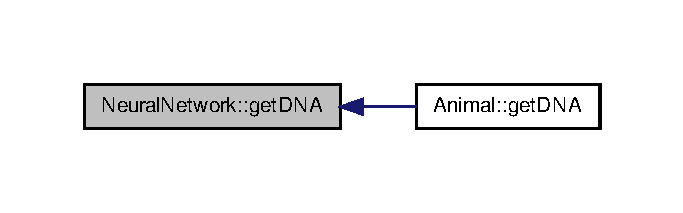
\includegraphics[width=328pt]{class_neural_network_abd6e6ec0a4500527150c127f0f8d7c23_icgraph}
\end{center}
\end{figure}


\hypertarget{class_neural_network_ace5b58e0174ef1f318db06f0b19f694b}{\index{Neural\-Network@{Neural\-Network}!init\-Layers@{init\-Layers}}
\index{init\-Layers@{init\-Layers}!NeuralNetwork@{Neural\-Network}}
\subsubsection[{init\-Layers}]{\setlength{\rightskip}{0pt plus 5cm}void Neural\-Network\-::init\-Layers (
\begin{DoxyParamCaption}
{}
\end{DoxyParamCaption}
)}}\label{class_neural_network_ace5b58e0174ef1f318db06f0b19f694b}


Initialisation of the different layers depending on inputs/outputs/config (for the hidden layer) 



Definition at line 9 of file neural\-\_\-network.\-cpp.



Here is the caller graph for this function\-:
\nopagebreak
\begin{figure}[H]
\begin{center}
\leavevmode
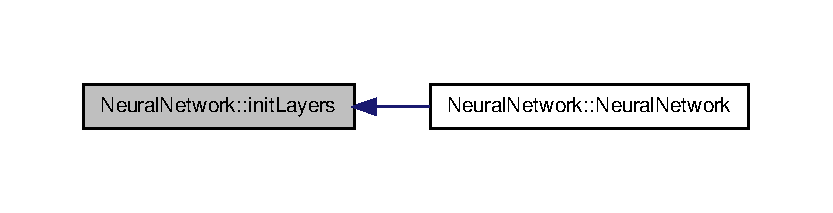
\includegraphics[width=350pt]{class_neural_network_ace5b58e0174ef1f318db06f0b19f694b_icgraph}
\end{center}
\end{figure}


\hypertarget{class_neural_network_a2daf940807763cd3d81661f93d99e6ba}{\index{Neural\-Network@{Neural\-Network}!run@{run}}
\index{run@{run}!NeuralNetwork@{Neural\-Network}}
\subsubsection[{run}]{\setlength{\rightskip}{0pt plus 5cm}std\-::vector$<$ float $>$ Neural\-Network\-::run (
\begin{DoxyParamCaption}
\item[{const std\-::vector$<$ float $>$}]{inputs}
\end{DoxyParamCaption}
)}}\label{class_neural_network_a2daf940807763cd3d81661f93d99e6ba}


Runs the calculation of the outputs array depending on the inputs. 


\begin{DoxyParams}{Parameters}
{\em inputs} & The inputs array \\
\hline
\end{DoxyParams}
\begin{DoxyReturn}{Returns}
The outpus array 
\end{DoxyReturn}


Definition at line 30 of file neural\-\_\-network.\-cpp.



Here is the caller graph for this function\-:
\nopagebreak
\begin{figure}[H]
\begin{center}
\leavevmode
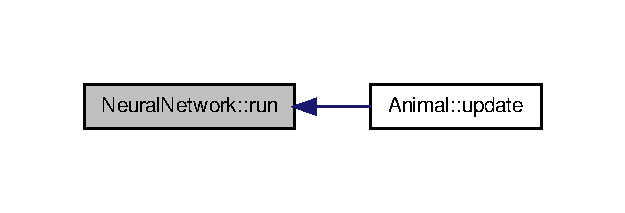
\includegraphics[width=300pt]{class_neural_network_a2daf940807763cd3d81661f93d99e6ba_icgraph}
\end{center}
\end{figure}


\hypertarget{class_neural_network_a38e8afa4eb8651b80c48b577ecdc6c4a}{\index{Neural\-Network@{Neural\-Network}!set\-D\-N\-A@{set\-D\-N\-A}}
\index{set\-D\-N\-A@{set\-D\-N\-A}!NeuralNetwork@{Neural\-Network}}
\subsubsection[{set\-D\-N\-A}]{\setlength{\rightskip}{0pt plus 5cm}void Neural\-Network\-::set\-D\-N\-A (
\begin{DoxyParamCaption}
\item[{const std\-::vector$<$ float $>$ \&}]{D\-N\-A}
\end{DoxyParamCaption}
)}}\label{class_neural_network_a38e8afa4eb8651b80c48b577ecdc6c4a}


Updates the D\-N\-A of all neurons with the new one, given by the genetics algorithm. 


\begin{DoxyParams}{Parameters}
{\em D\-N\-A} & The D\-N\-A to set \\
\hline
\end{DoxyParams}


Definition at line 55 of file neural\-\_\-network.\-cpp.



Here is the caller graph for this function\-:
\nopagebreak
\begin{figure}[H]
\begin{center}
\leavevmode
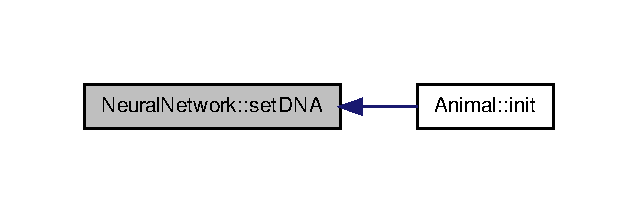
\includegraphics[width=306pt]{class_neural_network_a38e8afa4eb8651b80c48b577ecdc6c4a_icgraph}
\end{center}
\end{figure}




The documentation for this class was generated from the following files\-:\begin{DoxyCompactItemize}
\item 
src/\hyperlink{neural__network_8h}{neural\-\_\-network.\-h}\item 
src/\hyperlink{neural__network_8cpp}{neural\-\_\-network.\-cpp}\end{DoxyCompactItemize}

\hypertarget{class_neuron}{\section{Neuron Class Reference}
\label{class_neuron}\index{Neuron@{Neuron}}
}


The \hyperlink{class_neuron}{Neuron} class, with represents a singleton, without backprop or anything.  




{\ttfamily \#include $<$neuron.\-h$>$}

\subsection*{Public Member Functions}
\begin{DoxyCompactItemize}
\item 
\hyperlink{class_neuron_aac37e4753166ab39e0f4f6d90fdeda57}{Neuron} (unsigned int \-\_\-inputs\-Number)
\item 
\hyperlink{class_neuron_a94a250ce7e167760e593979b899745b1}{$\sim$\-Neuron} ()
\item 
void \hyperlink{class_neuron_abb3a85d2adf4a9c5a5b646c83086a2ae}{init\-Weights} ()
\begin{DoxyCompactList}\small\item\em Initializes all the weights with uniform rand values \mbox{[}-\/1; 1\mbox{]}. \end{DoxyCompactList}\item 
const float \hyperlink{class_neuron_a1d1bedb17ff3d87afcc282421579ad5f}{run} (const std\-::vector$<$ float $>$ inputs)
\begin{DoxyCompactList}\small\item\em Runs the calculation of the output value depending on the inputs. \end{DoxyCompactList}\item 
void \hyperlink{class_neuron_a873e07fce168dfde42961ea151593c9f}{set\-D\-N\-A} (const std\-::vector$<$ float $>$ \&D\-N\-A)
\begin{DoxyCompactList}\small\item\em Updates the D\-N\-A of the neuron with the new one given by the G\-A. \end{DoxyCompactList}\item 
std\-::vector$<$ float $>$ \hyperlink{class_neuron_a2626c0a0fa4dbca17dc7fd9b3b390c07}{get\-D\-N\-A} ()
\item 
unsigned int \hyperlink{class_neuron_a40d81d3ea3f2af3e2f3297533132fd31}{get\-D\-N\-A\-Size} () const 
\end{DoxyCompactItemize}


\subsection{Detailed Description}
The \hyperlink{class_neuron}{Neuron} class, with represents a singleton, without backprop or anything. 


\begin{DoxyParams}{Parameters}
{\em \-\_\-inputs\-Number} & The inputs number of the neuron\\
\hline
\end{DoxyParams}
The Neurons used in the projects are ultra simple percpetrons, without back-\/propagation or anything like it.

It uses sigmoids as an activation function, because floats are so cooler than bools (and much more C\-P\-U-\/intensive).

I'll let you check out Wikipedia if you need more info about how a perceptron work, or let you check out the \hyperlink{class_neural_network}{Neural\-Network} class, where I described a bit more how my Neural Networks worked. 

Definition at line 20 of file neuron.\-h.



\subsection{Constructor \& Destructor Documentation}
\hypertarget{class_neuron_aac37e4753166ab39e0f4f6d90fdeda57}{\index{Neuron@{Neuron}!Neuron@{Neuron}}
\index{Neuron@{Neuron}!Neuron@{Neuron}}
\subsubsection[{Neuron}]{\setlength{\rightskip}{0pt plus 5cm}Neuron\-::\-Neuron (
\begin{DoxyParamCaption}
\item[{unsigned int}]{\-\_\-inputs\-Number}
\end{DoxyParamCaption}
)}}\label{class_neuron_aac37e4753166ab39e0f4f6d90fdeda57}


Definition at line 3 of file neuron.\-cpp.



Here is the call graph for this function\-:\nopagebreak
\begin{figure}[H]
\begin{center}
\leavevmode
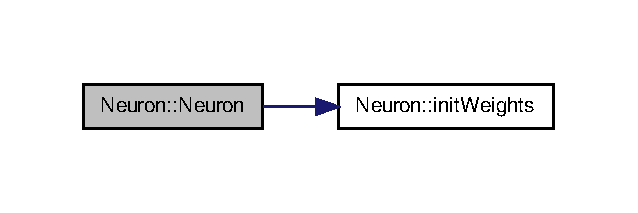
\includegraphics[width=306pt]{class_neuron_aac37e4753166ab39e0f4f6d90fdeda57_cgraph}
\end{center}
\end{figure}


\hypertarget{class_neuron_a94a250ce7e167760e593979b899745b1}{\index{Neuron@{Neuron}!$\sim$\-Neuron@{$\sim$\-Neuron}}
\index{$\sim$\-Neuron@{$\sim$\-Neuron}!Neuron@{Neuron}}
\subsubsection[{$\sim$\-Neuron}]{\setlength{\rightskip}{0pt plus 5cm}Neuron\-::$\sim$\-Neuron (
\begin{DoxyParamCaption}
{}
\end{DoxyParamCaption}
)}}\label{class_neuron_a94a250ce7e167760e593979b899745b1}


Definition at line 8 of file neuron.\-cpp.



\subsection{Member Function Documentation}
\hypertarget{class_neuron_a2626c0a0fa4dbca17dc7fd9b3b390c07}{\index{Neuron@{Neuron}!get\-D\-N\-A@{get\-D\-N\-A}}
\index{get\-D\-N\-A@{get\-D\-N\-A}!Neuron@{Neuron}}
\subsubsection[{get\-D\-N\-A}]{\setlength{\rightskip}{0pt plus 5cm}std\-::vector$<$ float $>$ Neuron\-::get\-D\-N\-A (
\begin{DoxyParamCaption}
{}
\end{DoxyParamCaption}
)}}\label{class_neuron_a2626c0a0fa4dbca17dc7fd9b3b390c07}
\begin{DoxyReturn}{Returns}
the D\-N\-A of the neuron, which is the array of its weights 
\end{DoxyReturn}


Definition at line 39 of file neuron.\-cpp.

\hypertarget{class_neuron_a40d81d3ea3f2af3e2f3297533132fd31}{\index{Neuron@{Neuron}!get\-D\-N\-A\-Size@{get\-D\-N\-A\-Size}}
\index{get\-D\-N\-A\-Size@{get\-D\-N\-A\-Size}!Neuron@{Neuron}}
\subsubsection[{get\-D\-N\-A\-Size}]{\setlength{\rightskip}{0pt plus 5cm}unsigned int Neuron\-::get\-D\-N\-A\-Size (
\begin{DoxyParamCaption}
{}
\end{DoxyParamCaption}
) const\hspace{0.3cm}{\ttfamily [inline]}}}\label{class_neuron_a40d81d3ea3f2af3e2f3297533132fd31}
\begin{DoxyReturn}{Returns}
The size of the D\-N\-A of the neuron 
\end{DoxyReturn}


Definition at line 57 of file neuron.\-h.

\hypertarget{class_neuron_abb3a85d2adf4a9c5a5b646c83086a2ae}{\index{Neuron@{Neuron}!init\-Weights@{init\-Weights}}
\index{init\-Weights@{init\-Weights}!Neuron@{Neuron}}
\subsubsection[{init\-Weights}]{\setlength{\rightskip}{0pt plus 5cm}void Neuron\-::init\-Weights (
\begin{DoxyParamCaption}
{}
\end{DoxyParamCaption}
)}}\label{class_neuron_abb3a85d2adf4a9c5a5b646c83086a2ae}


Initializes all the weights with uniform rand values \mbox{[}-\/1; 1\mbox{]}. 



Definition at line 10 of file neuron.\-cpp.



Here is the caller graph for this function\-:\nopagebreak
\begin{figure}[H]
\begin{center}
\leavevmode
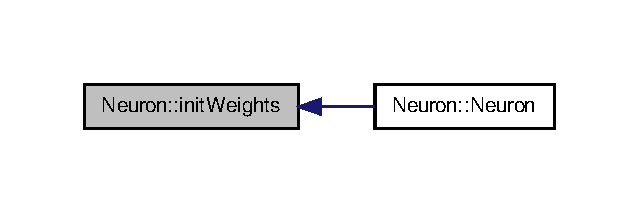
\includegraphics[width=306pt]{class_neuron_abb3a85d2adf4a9c5a5b646c83086a2ae_icgraph}
\end{center}
\end{figure}


\hypertarget{class_neuron_a1d1bedb17ff3d87afcc282421579ad5f}{\index{Neuron@{Neuron}!run@{run}}
\index{run@{run}!Neuron@{Neuron}}
\subsubsection[{run}]{\setlength{\rightskip}{0pt plus 5cm}const float Neuron\-::run (
\begin{DoxyParamCaption}
\item[{const std\-::vector$<$ float $>$}]{inputs}
\end{DoxyParamCaption}
)}}\label{class_neuron_a1d1bedb17ff3d87afcc282421579ad5f}


Runs the calculation of the output value depending on the inputs. 


\begin{DoxyParams}{Parameters}
{\em inputs} & The inputs array \\
\hline
\end{DoxyParams}
\begin{DoxyReturn}{Returns}
The output value
\end{DoxyReturn}
To compute the output, we make the linear combination of weights and inputs \-: sum = weights $\ast$ inputs Then, we apply an activation function to sum, so that it stays within the interval \mbox{[}-\/1; 1\mbox{]} In our case, we use a sigmoid, which inclination is determined by Neuron\-Sigmoid in config.\-cfg 

Definition at line 21 of file neuron.\-cpp.

\hypertarget{class_neuron_a873e07fce168dfde42961ea151593c9f}{\index{Neuron@{Neuron}!set\-D\-N\-A@{set\-D\-N\-A}}
\index{set\-D\-N\-A@{set\-D\-N\-A}!Neuron@{Neuron}}
\subsubsection[{set\-D\-N\-A}]{\setlength{\rightskip}{0pt plus 5cm}void Neuron\-::set\-D\-N\-A (
\begin{DoxyParamCaption}
\item[{const std\-::vector$<$ float $>$ \&}]{D\-N\-A}
\end{DoxyParamCaption}
)}}\label{class_neuron_a873e07fce168dfde42961ea151593c9f}


Updates the D\-N\-A of the neuron with the new one given by the G\-A. 


\begin{DoxyParams}{Parameters}
{\em D\-N\-A} & The new piece of A\-D\-N\\
\hline
\end{DoxyParams}
We simply replace the actual weights by the ones given by the D\-N\-A 

Definition at line 34 of file neuron.\-cpp.



The documentation for this class was generated from the following files\-:\begin{DoxyCompactItemize}
\item 
src/\hyperlink{neuron_8h}{neuron.\-h}\item 
src/\hyperlink{neuron_8cpp}{neuron.\-cpp}\end{DoxyCompactItemize}

\hypertarget{struct_species}{\section{Species Struct Reference}
\label{struct_species}\index{Species@{Species}}
}


Structure containing a species of animals.  




{\ttfamily \#include $<$entity\-\_\-manager.\-h$>$}

\subsection*{Public Attributes}
\begin{DoxyCompactItemize}
\item 
std\-::vector$<$ \hyperlink{class_animal}{Animal} $\ast$ $>$ \hyperlink{struct_species_ad608dc238745c2120e642fe5222d0afb}{tab}
\begin{DoxyCompactList}\small\item\em The animals tab. \end{DoxyCompactList}\end{DoxyCompactItemize}


\subsection{Detailed Description}
Structure containing a species of animals. 

Definition at line 17 of file entity\-\_\-manager.\-h.



\subsection{Member Data Documentation}
\hypertarget{struct_species_ad608dc238745c2120e642fe5222d0afb}{\index{Species@{Species}!tab@{tab}}
\index{tab@{tab}!Species@{Species}}
\subsubsection[{tab}]{\setlength{\rightskip}{0pt plus 5cm}std\-::vector$<${\bf Animal}$\ast$$>$ Species\-::tab}}\label{struct_species_ad608dc238745c2120e642fe5222d0afb}


The animals tab. 



Definition at line 18 of file entity\-\_\-manager.\-h.



The documentation for this struct was generated from the following file\-:\begin{DoxyCompactItemize}
\item 
src/\hyperlink{entity__manager_8h}{entity\-\_\-manager.\-h}\end{DoxyCompactItemize}

\hypertarget{struct_vect2i}{\section{Vect2i Struct Reference}
\label{struct_vect2i}\index{Vect2i@{Vect2i}}
}


{\ttfamily \#include $<$utils.\-h$>$}

\subsection*{Public Member Functions}
\begin{DoxyCompactItemize}
\item 
\hyperlink{struct_vect2i_a141de752973cb8b63e70e16f84653f03}{Vect2i} (int \-\_\-x=0, int \-\_\-y=0)
\end{DoxyCompactItemize}
\subsection*{Public Attributes}
\begin{DoxyCompactItemize}
\item 
int \hyperlink{struct_vect2i_ae76ced0cba575b16f9de72e78828122b}{x}
\item 
int \hyperlink{struct_vect2i_a32d99812cd2cccca2b9751259783b699}{y}
\end{DoxyCompactItemize}


\subsection{Detailed Description}


Definition at line 32 of file utils.\-h.



\subsection{Constructor \& Destructor Documentation}
\hypertarget{struct_vect2i_a141de752973cb8b63e70e16f84653f03}{\index{Vect2i@{Vect2i}!Vect2i@{Vect2i}}
\index{Vect2i@{Vect2i}!Vect2i@{Vect2i}}
\subsubsection[{Vect2i}]{\setlength{\rightskip}{0pt plus 5cm}Vect2i\-::\-Vect2i (
\begin{DoxyParamCaption}
\item[{int}]{\-\_\-x = {\ttfamily 0}, }
\item[{int}]{\-\_\-y = {\ttfamily 0}}
\end{DoxyParamCaption}
)\hspace{0.3cm}{\ttfamily [inline]}}}\label{struct_vect2i_a141de752973cb8b63e70e16f84653f03}


Definition at line 36 of file utils.\-h.



\subsection{Member Data Documentation}
\hypertarget{struct_vect2i_ae76ced0cba575b16f9de72e78828122b}{\index{Vect2i@{Vect2i}!x@{x}}
\index{x@{x}!Vect2i@{Vect2i}}
\subsubsection[{x}]{\setlength{\rightskip}{0pt plus 5cm}int Vect2i\-::x}}\label{struct_vect2i_ae76ced0cba575b16f9de72e78828122b}


Definition at line 33 of file utils.\-h.

\hypertarget{struct_vect2i_a32d99812cd2cccca2b9751259783b699}{\index{Vect2i@{Vect2i}!y@{y}}
\index{y@{y}!Vect2i@{Vect2i}}
\subsubsection[{y}]{\setlength{\rightskip}{0pt plus 5cm}int Vect2i\-::y}}\label{struct_vect2i_a32d99812cd2cccca2b9751259783b699}


Definition at line 34 of file utils.\-h.



The documentation for this struct was generated from the following file\-:\begin{DoxyCompactItemize}
\item 
src/\hyperlink{utils_8h}{utils.\-h}\end{DoxyCompactItemize}

\chapter{File Documentation}
\hypertarget{animal_8cpp}{\section{src/animal.cpp File Reference}
\label{animal_8cpp}\index{src/animal.\-cpp@{src/animal.\-cpp}}
}
{\ttfamily \#include \char`\"{}animal.\-h\char`\"{}}\\*
Include dependency graph for animal.\-cpp\-:\nopagebreak
\begin{figure}[H]
\begin{center}
\leavevmode
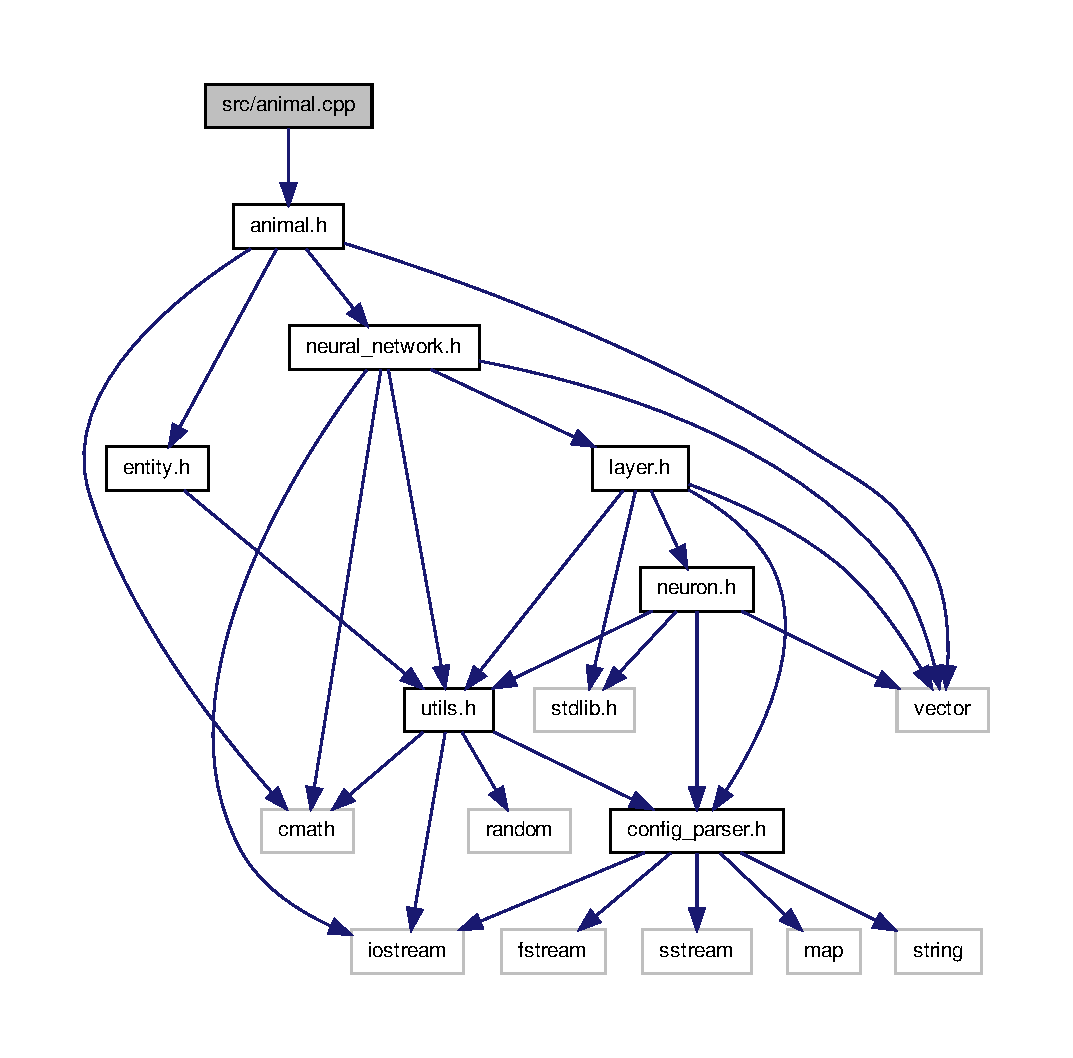
\includegraphics[width=350pt]{animal_8cpp__incl}
\end{center}
\end{figure}
\subsection*{Macros}
\begin{DoxyCompactItemize}
\item 
\#define \hyperlink{animal_8cpp_af66075a058e499320a380abe3bea31f4}{S\-E\-U\-I\-L\-\_\-\-A\-T\-T\-A\-C\-K\-I\-N\-G}~0.\-9f
\end{DoxyCompactItemize}


\subsection{Macro Definition Documentation}
\hypertarget{animal_8cpp_af66075a058e499320a380abe3bea31f4}{\index{animal.\-cpp@{animal.\-cpp}!S\-E\-U\-I\-L\-\_\-\-A\-T\-T\-A\-C\-K\-I\-N\-G@{S\-E\-U\-I\-L\-\_\-\-A\-T\-T\-A\-C\-K\-I\-N\-G}}
\index{S\-E\-U\-I\-L\-\_\-\-A\-T\-T\-A\-C\-K\-I\-N\-G@{S\-E\-U\-I\-L\-\_\-\-A\-T\-T\-A\-C\-K\-I\-N\-G}!animal.cpp@{animal.\-cpp}}
\subsubsection[{S\-E\-U\-I\-L\-\_\-\-A\-T\-T\-A\-C\-K\-I\-N\-G}]{\setlength{\rightskip}{0pt plus 5cm}\#define S\-E\-U\-I\-L\-\_\-\-A\-T\-T\-A\-C\-K\-I\-N\-G~0.\-9f}}\label{animal_8cpp_af66075a058e499320a380abe3bea31f4}


Definition at line 3 of file animal.\-cpp.


\hypertarget{animal_8h}{\section{src/animal.h File Reference}
\label{animal_8h}\index{src/animal.\-h@{src/animal.\-h}}
}
{\ttfamily \#include $<$vector$>$}\\*
{\ttfamily \#include $<$cmath$>$}\\*
{\ttfamily \#include \char`\"{}entity.\-h\char`\"{}}\\*
{\ttfamily \#include \char`\"{}neural\-\_\-network.\-h\char`\"{}}\\*
Include dependency graph for animal.\-h\-:\nopagebreak
\begin{figure}[H]
\begin{center}
\leavevmode
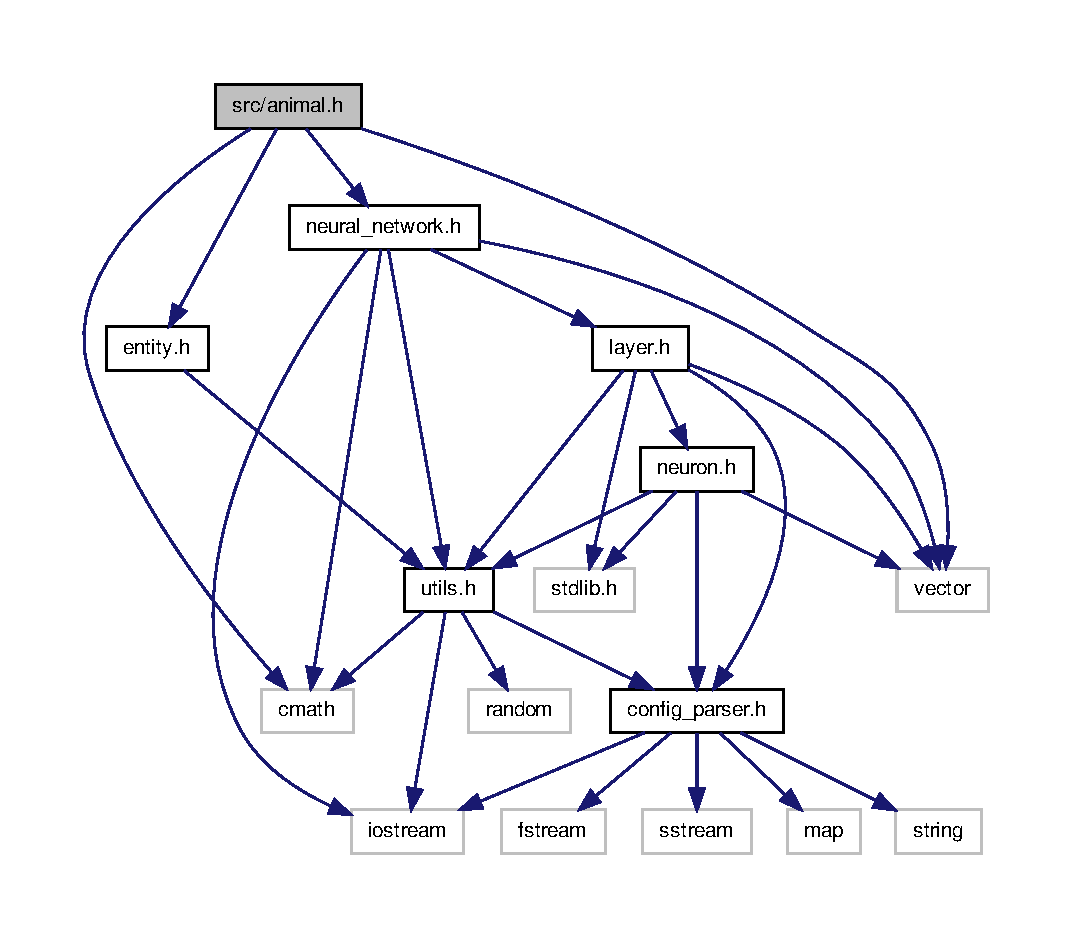
\includegraphics[width=350pt]{animal_8h__incl}
\end{center}
\end{figure}
This graph shows which files directly or indirectly include this file\-:\nopagebreak
\begin{figure}[H]
\begin{center}
\leavevmode
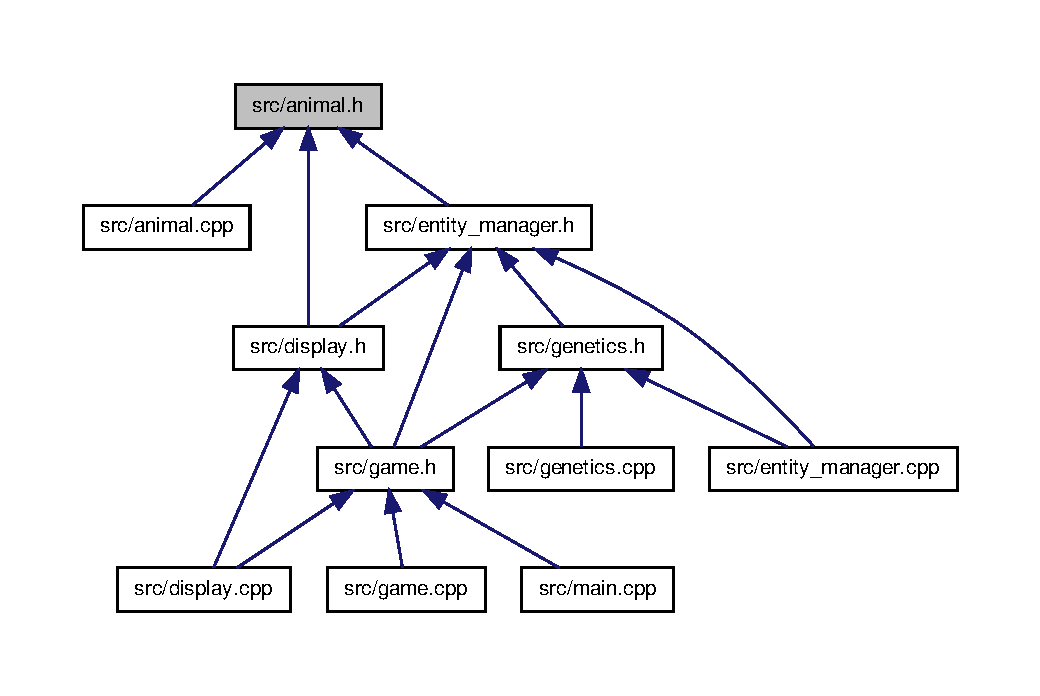
\includegraphics[width=350pt]{animal_8h__dep__incl}
\end{center}
\end{figure}
\subsection*{Classes}
\begin{DoxyCompactItemize}
\item 
class \hyperlink{class_animal}{Animal}
\begin{DoxyCompactList}\small\item\em Class representing an animal, containing a brain (\hyperlink{class_neural_network}{Neural\-Network}), that changes the animal's state given game inputs. \end{DoxyCompactList}\end{DoxyCompactItemize}

\hypertarget{config__parser_8cpp}{\section{src/config\-\_\-parser.cpp File Reference}
\label{config__parser_8cpp}\index{src/config\-\_\-parser.\-cpp@{src/config\-\_\-parser.\-cpp}}
}
{\ttfamily \#include \char`\"{}config\-\_\-parser.\-h\char`\"{}}\\*
<<<<<<< HEAD
Include dependency graph for config\-\_\-parser.\-cpp\-:
\nopagebreak
=======
Include dependency graph for config\-\_\-parser.\-cpp\-:\nopagebreak
>>>>>>> master
\begin{figure}[H]
\begin{center}
\leavevmode
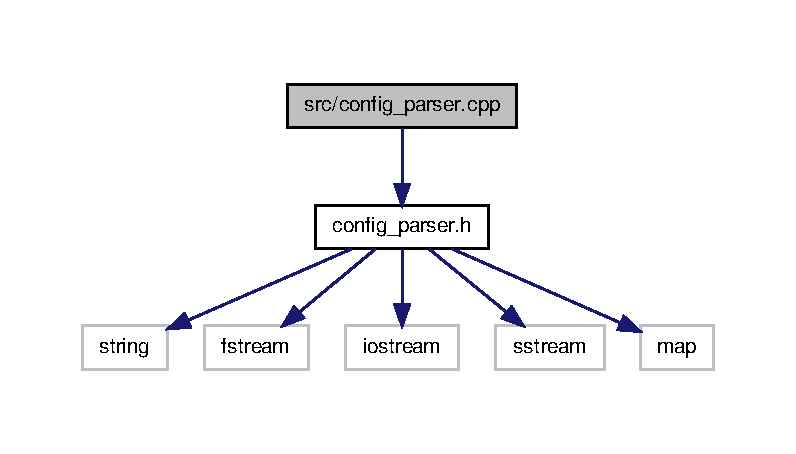
\includegraphics[width=350pt]{config__parser_8cpp__incl}
\end{center}
\end{figure}
\subsection*{Macros}
\begin{DoxyCompactItemize}
\item 
\#define \hyperlink{config__parser_8cpp_ad72dbcf6d0153db1b8d8a58001feed83}{D\-E\-B\-U\-G}~0
\end{DoxyCompactItemize}


\subsection{Macro Definition Documentation}
\hypertarget{config__parser_8cpp_ad72dbcf6d0153db1b8d8a58001feed83}{\index{config\-\_\-parser.\-cpp@{config\-\_\-parser.\-cpp}!D\-E\-B\-U\-G@{D\-E\-B\-U\-G}}
\index{D\-E\-B\-U\-G@{D\-E\-B\-U\-G}!config_parser.cpp@{config\-\_\-parser.\-cpp}}
\subsubsection[{D\-E\-B\-U\-G}]{\setlength{\rightskip}{0pt plus 5cm}\#define D\-E\-B\-U\-G~0}}\label{config__parser_8cpp_ad72dbcf6d0153db1b8d8a58001feed83}


Definition at line 5 of file config\-\_\-parser.\-cpp.


\hypertarget{config__parser_8h}{\section{src/config\-\_\-parser.h File Reference}
\label{config__parser_8h}\index{src/config\-\_\-parser.\-h@{src/config\-\_\-parser.\-h}}
}
{\ttfamily \#include $<$string$>$}\\*
{\ttfamily \#include $<$fstream$>$}\\*
{\ttfamily \#include $<$iostream$>$}\\*
{\ttfamily \#include $<$sstream$>$}\\*
{\ttfamily \#include $<$map$>$}\\*
Include dependency graph for config\-\_\-parser.\-h\-:
\nopagebreak
\begin{figure}[H]
\begin{center}
\leavevmode
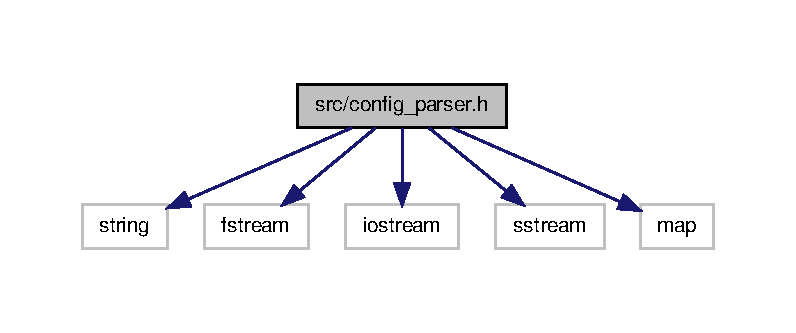
\includegraphics[width=350pt]{config__parser_8h__incl}
\end{center}
\end{figure}
This graph shows which files directly or indirectly include this file\-:
\nopagebreak
\begin{figure}[H]
\begin{center}
\leavevmode
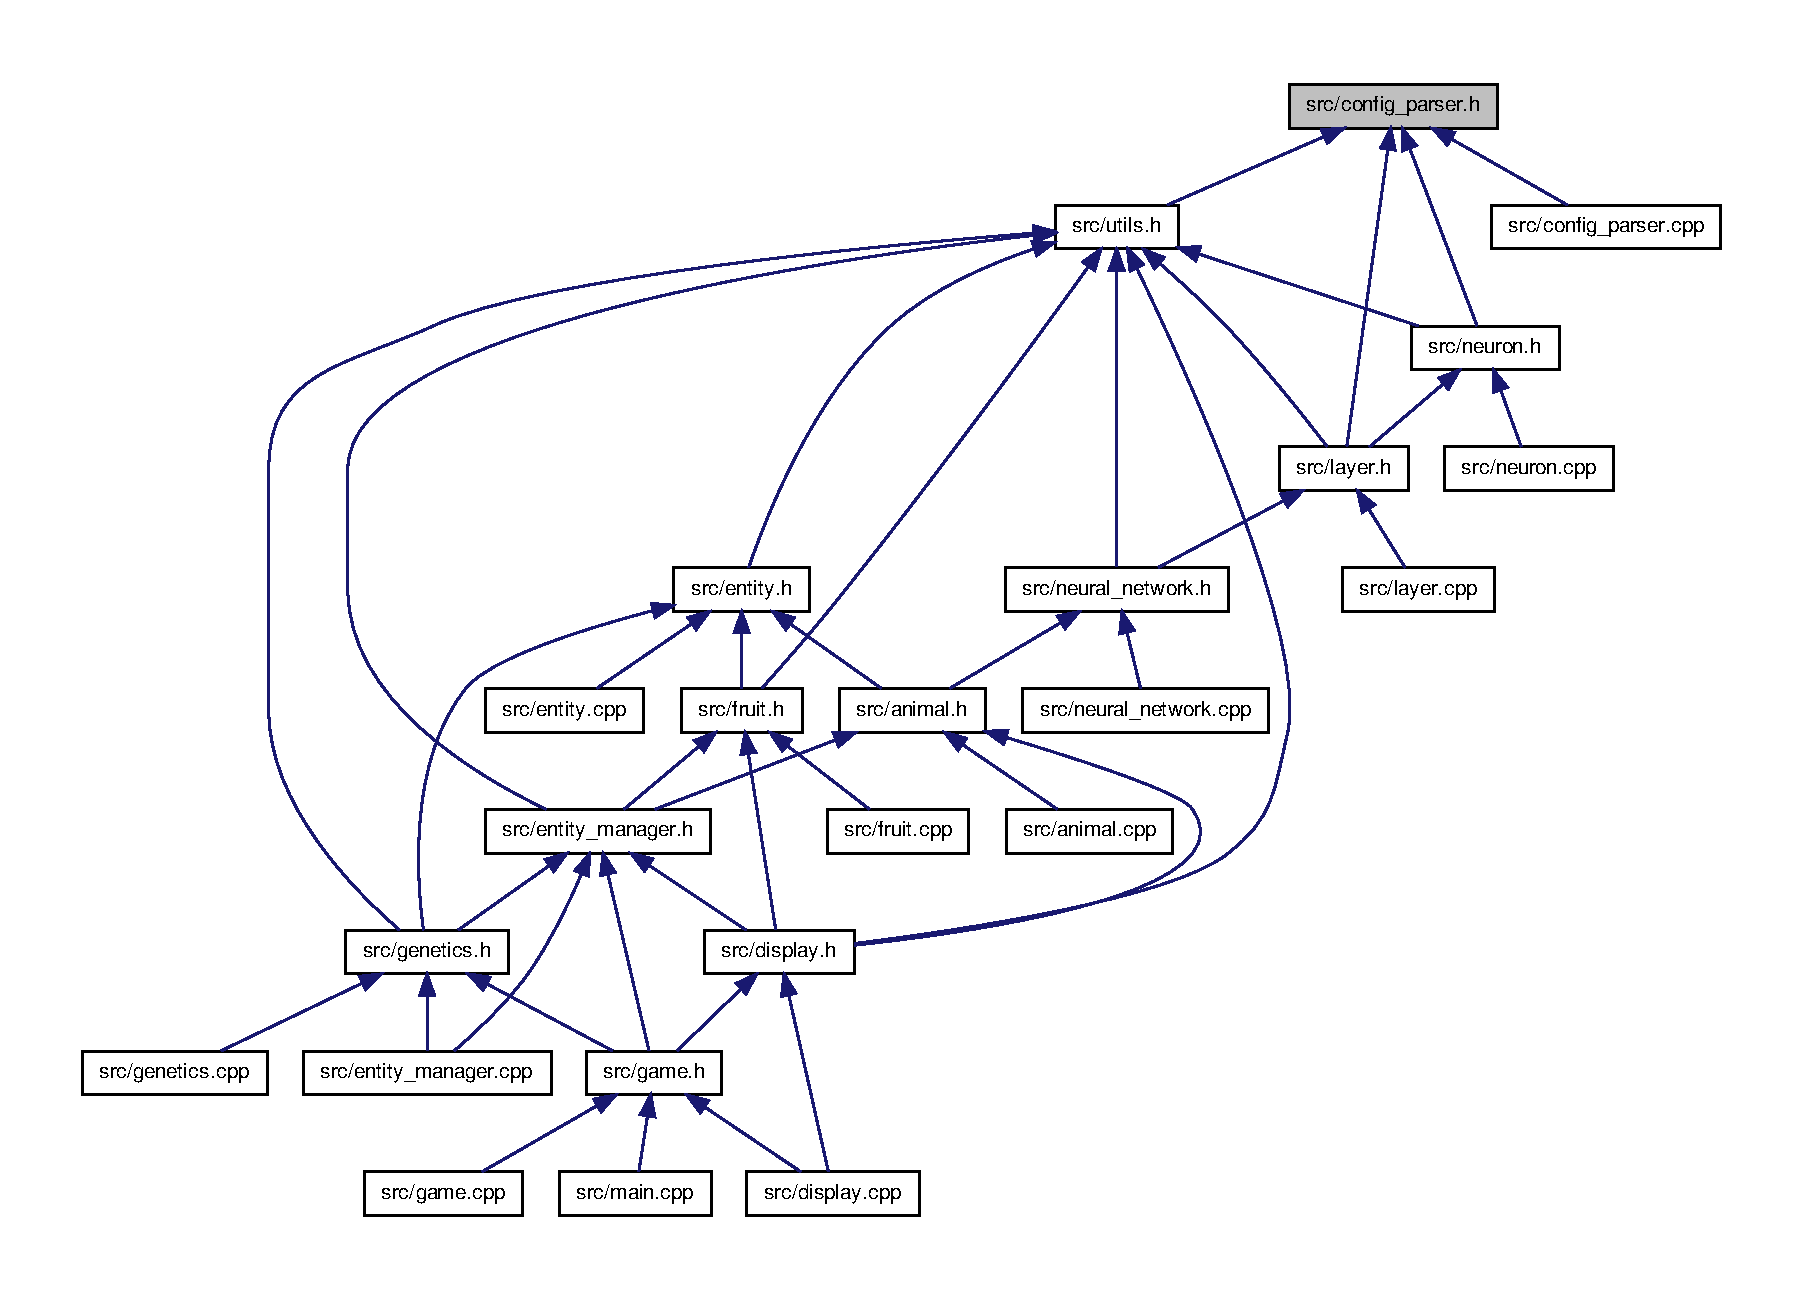
\includegraphics[width=350pt]{config__parser_8h__dep__incl}
\end{center}
\end{figure}
\subsection*{Classes}
\begin{DoxyCompactItemize}
\item 
class \hyperlink{class_config_parser}{Config\-Parser}
\end{DoxyCompactItemize}

\hypertarget{display_8cpp}{\section{src/display.cpp File Reference}
\label{display_8cpp}\index{src/display.\-cpp@{src/display.\-cpp}}
}
{\ttfamily \#include \char`\"{}display.\-h\char`\"{}}\\*
{\ttfamily \#include \char`\"{}game.\-h\char`\"{}}\\*
Include dependency graph for display.\-cpp\-:\nopagebreak
\begin{figure}[H]
\begin{center}
\leavevmode
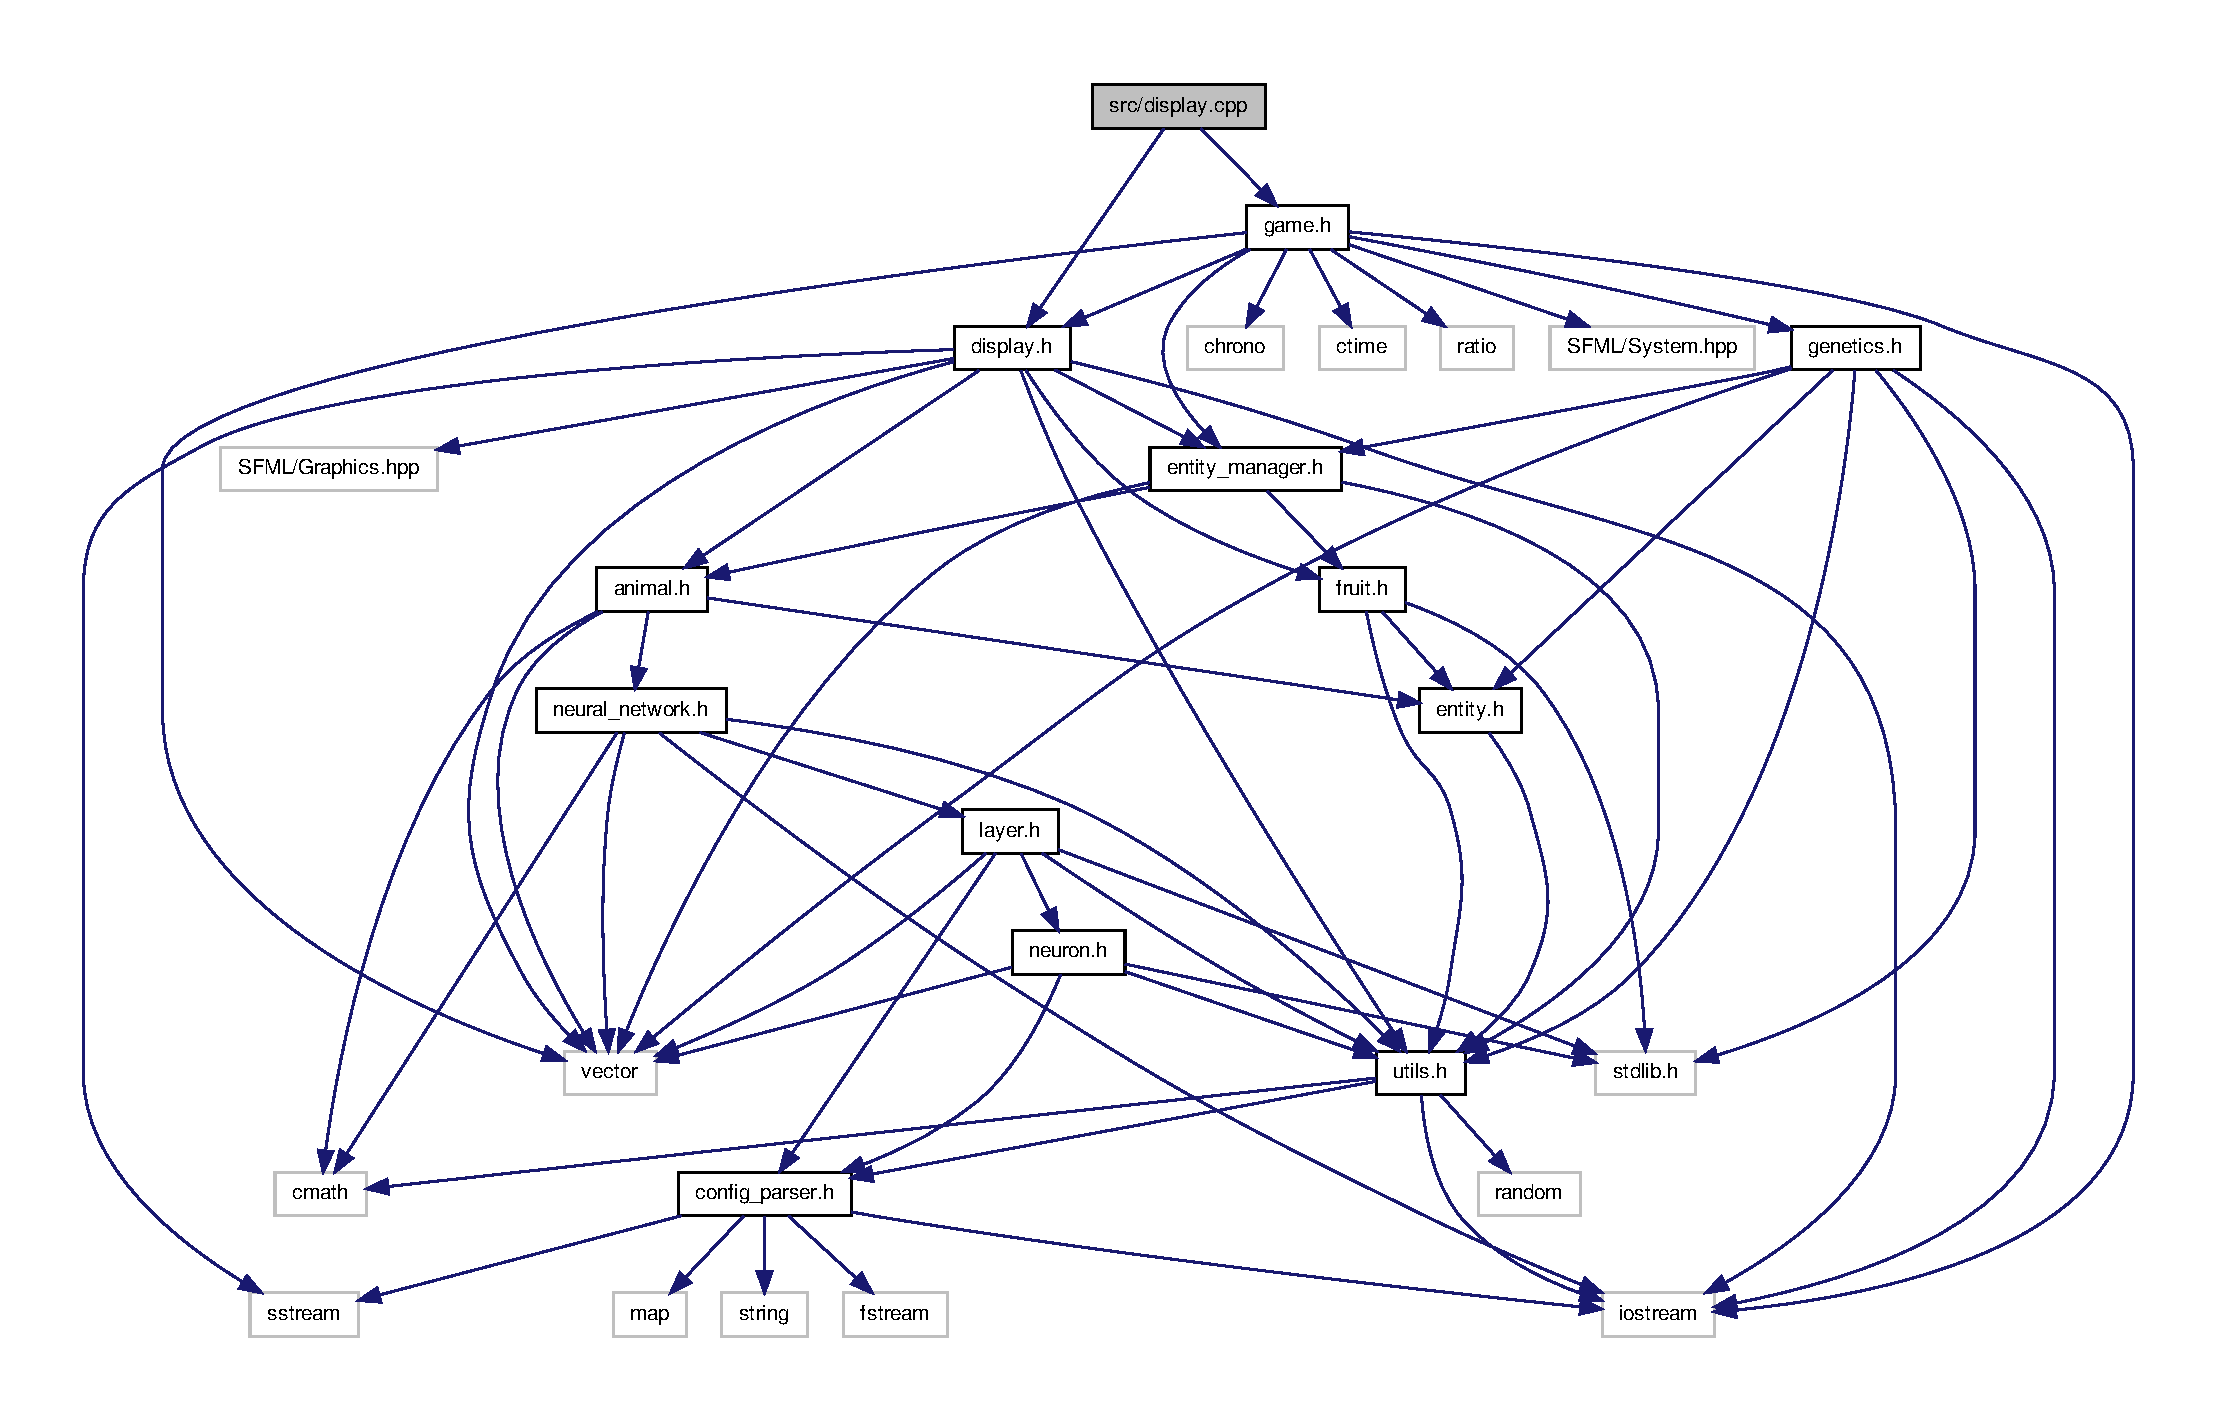
\includegraphics[width=350pt]{display_8cpp__incl}
\end{center}
\end{figure}

\hypertarget{display_8h}{\section{src/display.h File Reference}
\label{display_8h}\index{src/display.\-h@{src/display.\-h}}
}
{\ttfamily \#include $<$vector$>$}\\*
{\ttfamily \#include $<$iostream$>$}\\*
{\ttfamily \#include $<$S\-F\-M\-L/\-Graphics.\-hpp$>$}\\*
{\ttfamily \#include $<$sstream$>$}\\*
{\ttfamily \#include \char`\"{}entity\-\_\-manager.\-h\char`\"{}}\\*
{\ttfamily \#include \char`\"{}utils.\-h\char`\"{}}\\*
{\ttfamily \#include \char`\"{}animal.\-h\char`\"{}}\\*
{\ttfamily \#include \char`\"{}fruit.\-h\char`\"{}}\\*
<<<<<<< HEAD
Include dependency graph for display.\-h\-:
\nopagebreak
=======
Include dependency graph for display.\-h\-:\nopagebreak
>>>>>>> master
\begin{figure}[H]
\begin{center}
\leavevmode
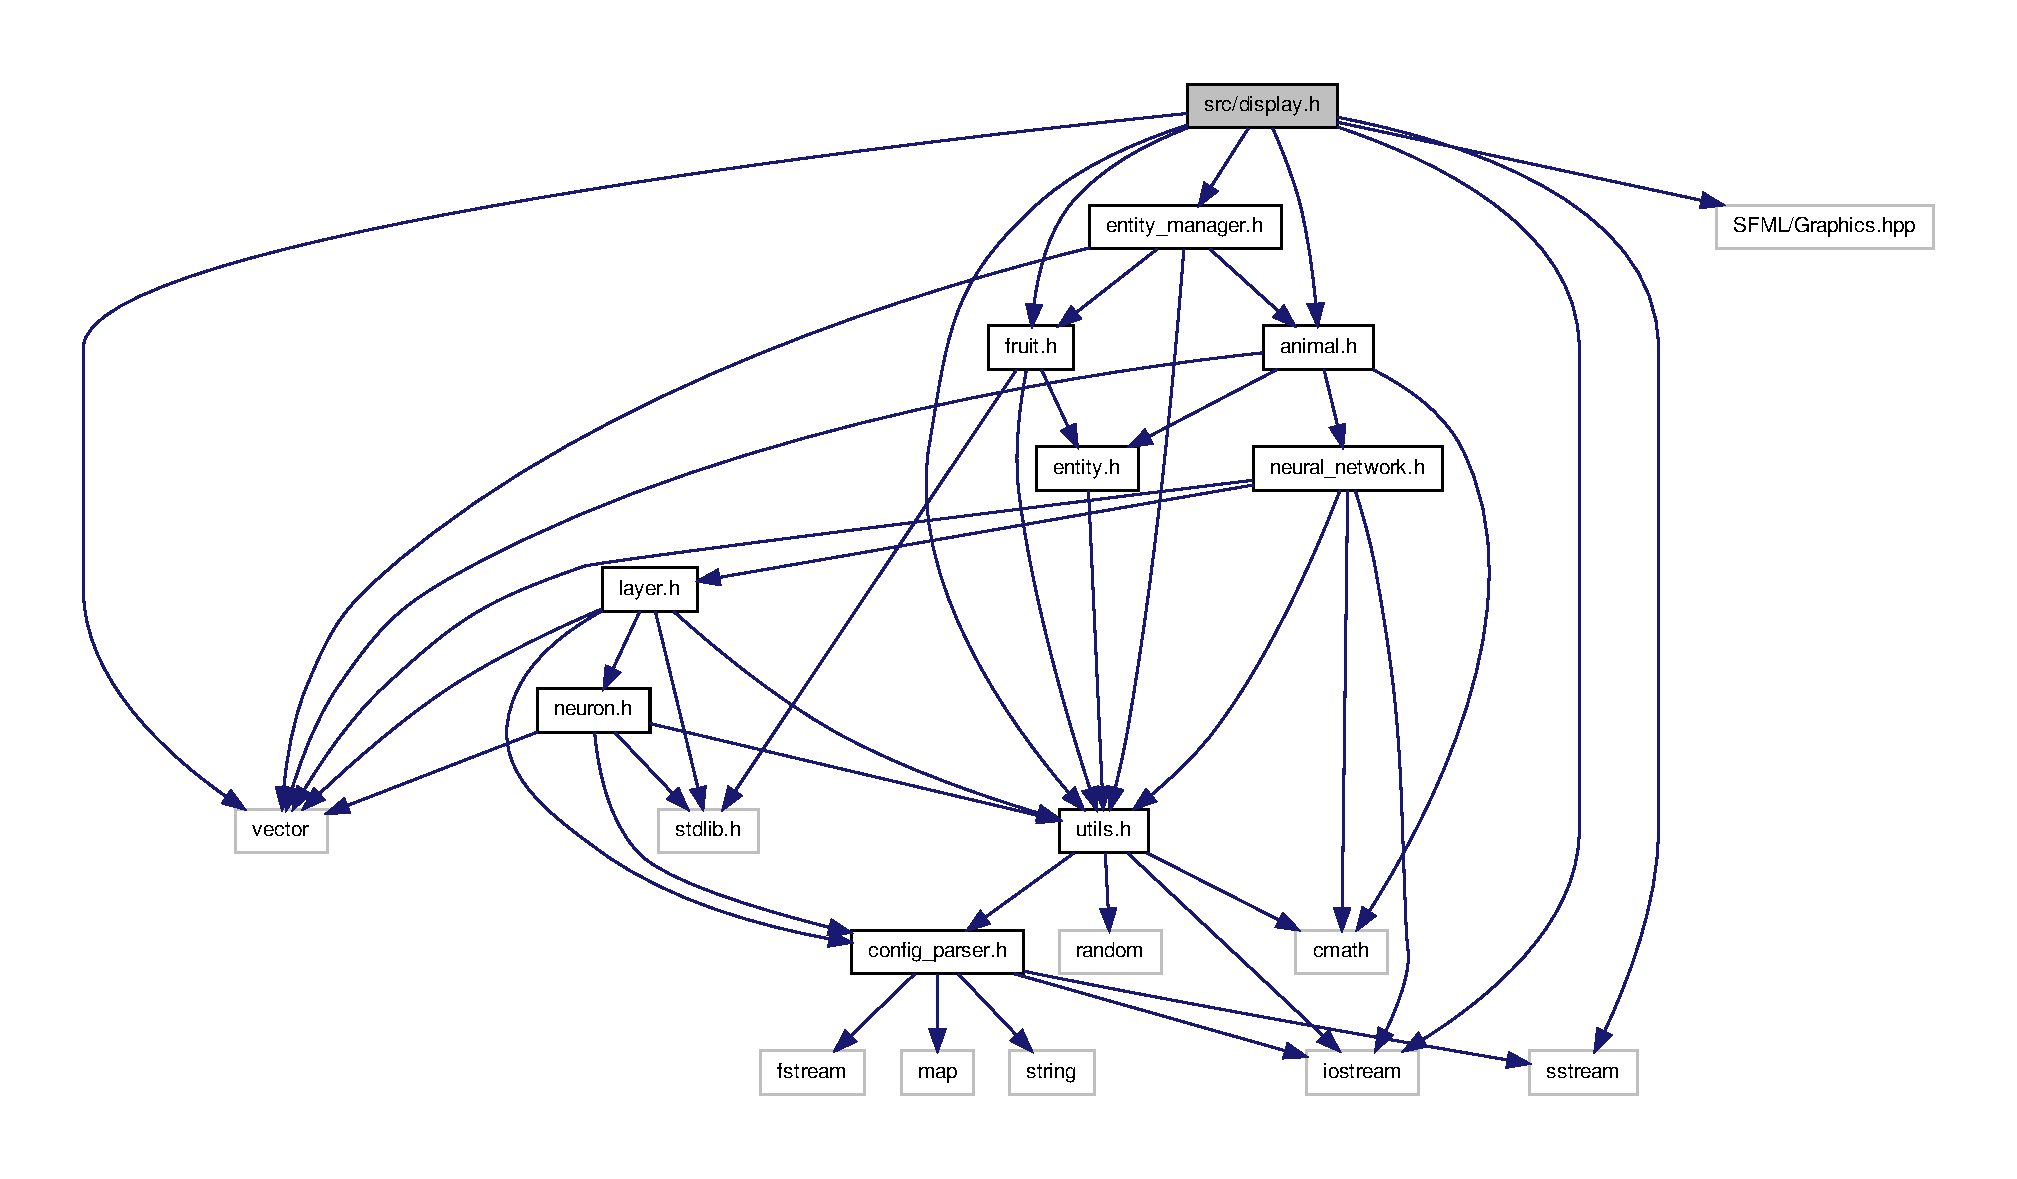
\includegraphics[width=350pt]{display_8h__incl}
\end{center}
\end{figure}
<<<<<<< HEAD
This graph shows which files directly or indirectly include this file\-:
\nopagebreak
=======
This graph shows which files directly or indirectly include this file\-:\nopagebreak
>>>>>>> master
\begin{figure}[H]
\begin{center}
\leavevmode
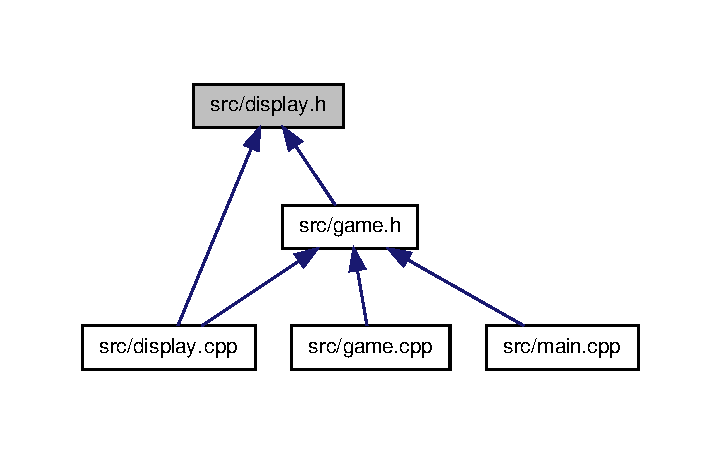
\includegraphics[width=346pt]{display_8h__dep__incl}
\end{center}
\end{figure}
\subsection*{Classes}
\begin{DoxyCompactItemize}
\item 
class \hyperlink{class_display}{Display}
<<<<<<< HEAD
\begin{DoxyCompactList}\small\item\em Class handling all the display/event engine. Only S\-F\-M\-L user with \hyperlink{class_game}{Game}. \end{DoxyCompactList}\end{DoxyCompactItemize}


\subsection{Detailed Description}
\begin{DoxyAuthor}{Author}
Adrien Luxey 
\end{DoxyAuthor}


Definition in file \hyperlink{display_8h_source}{display.\-h}.

=======
\begin{DoxyCompactList}\small\item\em Class handling every display aspect of the game. \end{DoxyCompactList}\end{DoxyCompactItemize}
>>>>>>> master

\hypertarget{entity_8cpp}{\section{src/entity.cpp File Reference}
\label{entity_8cpp}\index{src/entity.\-cpp@{src/entity.\-cpp}}
}
{\ttfamily \#include \char`\"{}entity.\-h\char`\"{}}\\*
Include dependency graph for entity.\-cpp\-:
\nopagebreak
\begin{figure}[H]
\begin{center}
\leavevmode
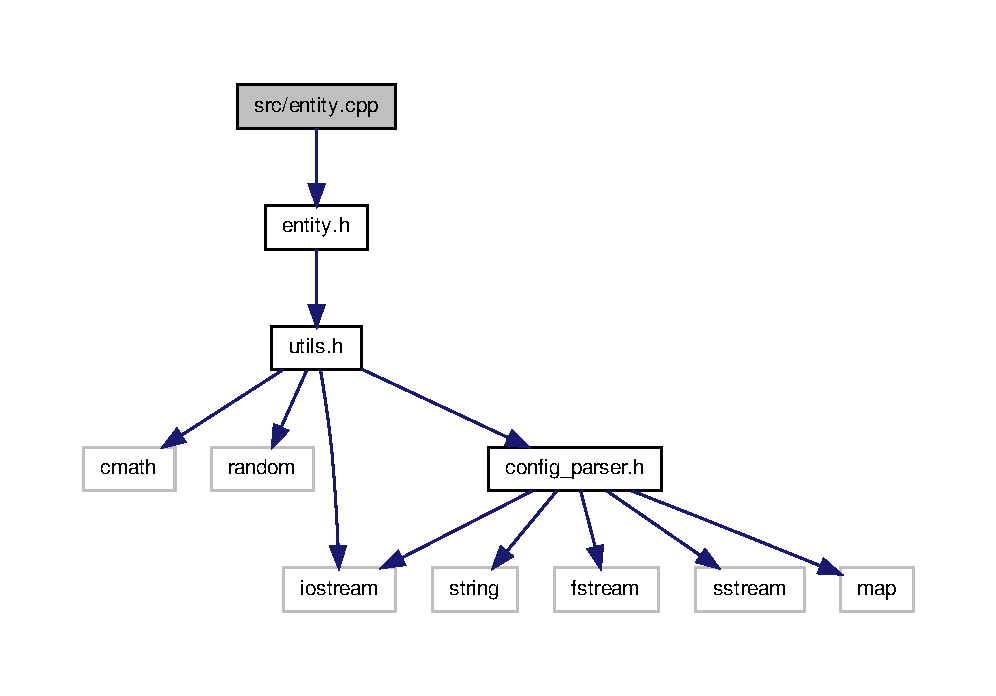
\includegraphics[width=350pt]{entity_8cpp__incl}
\end{center}
\end{figure}

\hypertarget{entity_8h}{\section{src/entity.h File Reference}
\label{entity_8h}\index{src/entity.\-h@{src/entity.\-h}}
}
{\ttfamily \#include \char`\"{}utils.\-h\char`\"{}}\\*
Include dependency graph for entity.\-h\-:\nopagebreak
\begin{figure}[H]
\begin{center}
\leavevmode
\includegraphics[width=350pt]{entity_8h__incl}
\end{center}
\end{figure}
This graph shows which files directly or indirectly include this file\-:\nopagebreak
\begin{figure}[H]
\begin{center}
\leavevmode
\includegraphics[width=350pt]{entity_8h__dep__incl}
\end{center}
\end{figure}
\subsection*{Classes}
\begin{DoxyCompactItemize}
\item 
class \hyperlink{class_entity}{Entity}
\begin{DoxyCompactList}\small\item\em Abstract class represtenting any displayable physical object of the game. \end{DoxyCompactList}\end{DoxyCompactItemize}

\hypertarget{entity__manager_8cpp}{\section{src/entity\-\_\-manager.cpp File Reference}
\label{entity__manager_8cpp}\index{src/entity\-\_\-manager.\-cpp@{src/entity\-\_\-manager.\-cpp}}
}
{\ttfamily \#include \char`\"{}entity\-\_\-manager.\-h\char`\"{}}\\*
{\ttfamily \#include \char`\"{}genetics.\-h\char`\"{}}\\*
Include dependency graph for entity\-\_\-manager.\-cpp\-:\nopagebreak
\begin{figure}[H]
\begin{center}
\leavevmode
\includegraphics[width=350pt]{entity__manager_8cpp__incl}
\end{center}
\end{figure}

\hypertarget{entity__manager_8h}{\section{src/entity\-\_\-manager.h File Reference}
\label{entity__manager_8h}\index{src/entity\-\_\-manager.\-h@{src/entity\-\_\-manager.\-h}}
}
{\ttfamily \#include $<$vector$>$}\\*
{\ttfamily \#include \char`\"{}utils.\-h\char`\"{}}\\*
{\ttfamily \#include \char`\"{}fruit.\-h\char`\"{}}\\*
{\ttfamily \#include \char`\"{}animal.\-h\char`\"{}}\\*
Include dependency graph for entity\-\_\-manager.\-h\-:\nopagebreak
\begin{figure}[H]
\begin{center}
\leavevmode
\includegraphics[width=350pt]{entity__manager_8h__incl}
\end{center}
\end{figure}
This graph shows which files directly or indirectly include this file\-:
\nopagebreak
\begin{figure}[H]
\begin{center}
\leavevmode
\includegraphics[width=350pt]{entity__manager_8h__dep__incl}
\end{center}
\end{figure}
\subsection*{Classes}
\begin{DoxyCompactItemize}
\item 
struct \hyperlink{struct_species}{Species}
\begin{DoxyCompactList}\small\item\em Structure containing a species of animals. \end{DoxyCompactList}\item 
class \hyperlink{class_entity_manager}{Entity\-Manager}
\begin{DoxyCompactList}\small\item\em Handles the entities, their relations, updates, and all the game mecanics. \end{DoxyCompactList}\end{DoxyCompactItemize}
\subsection*{Typedefs}
\begin{DoxyCompactItemize}
\item 
typedef struct \hyperlink{struct_species}{Species} \hyperlink{entity__manager_8h_a0832728b7db46fc23415523bebbb91d8}{Species}
\begin{DoxyCompactList}\small\item\em Structure containing a species of animals. \end{DoxyCompactList}\end{DoxyCompactItemize}


\subsection{Detailed Description}
\begin{DoxyAuthor}{Author}
Adrien Luxey 
\end{DoxyAuthor}


Definition in file \hyperlink{entity__manager_8h_source}{entity\-\_\-manager.\-h}.



\subsection{Typedef Documentation}
\hypertarget{entity__manager_8h_a0832728b7db46fc23415523bebbb91d8}{\index{entity\-\_\-manager.\-h@{entity\-\_\-manager.\-h}!Species@{Species}}
\index{Species@{Species}!entity_manager.h@{entity\-\_\-manager.\-h}}
\subsubsection[{Species}]{\setlength{\rightskip}{0pt plus 5cm}typedef struct {\bf Species}  {\bf Species}}}\label{entity__manager_8h_a0832728b7db46fc23415523bebbb91d8}


Structure containing a species of animals. 


\hypertarget{fruit_8cpp}{\section{src/fruit.cpp File Reference}
\label{fruit_8cpp}\index{src/fruit.\-cpp@{src/fruit.\-cpp}}
}
{\ttfamily \#include \char`\"{}fruit.\-h\char`\"{}}\\*
Include dependency graph for fruit.\-cpp\-:
\nopagebreak
\begin{figure}[H]
\begin{center}
\leavevmode
\includegraphics[width=350pt]{fruit_8cpp__incl}
\end{center}
\end{figure}

\hypertarget{fruit_8h}{\section{src/fruit.h File Reference}
\label{fruit_8h}\index{src/fruit.\-h@{src/fruit.\-h}}
}
{\ttfamily \#include $<$stdlib.\-h$>$}\\*
{\ttfamily \#include \char`\"{}utils.\-h\char`\"{}}\\*
{\ttfamily \#include \char`\"{}entity.\-h\char`\"{}}\\*
Include dependency graph for fruit.\-h\-:\nopagebreak
\begin{figure}[H]
\begin{center}
\leavevmode
\includegraphics[width=350pt]{fruit_8h__incl}
\end{center}
\end{figure}
This graph shows which files directly or indirectly include this file\-:
\nopagebreak
\begin{figure}[H]
\begin{center}
\leavevmode
\includegraphics[width=350pt]{fruit_8h__dep__incl}
\end{center}
\end{figure}
\subsection*{Classes}
\begin{DoxyCompactItemize}
\item 
struct \hyperlink{struct_bush}{Bush}
\begin{DoxyCompactList}\small\item\em Structure representig a bush \-: point and size where fruits have high probabylity to appear. \end{DoxyCompactList}\item 
class \hyperlink{class_fruit}{Fruit}
\begin{DoxyCompactList}\small\item\em class representing a fruit \-: static element that can be eaten by an animal \end{DoxyCompactList}\end{DoxyCompactItemize}
\subsection*{Typedefs}
\begin{DoxyCompactItemize}
\item 
typedef struct \hyperlink{struct_bush}{Bush} \hyperlink{fruit_8h_a821849b8b231998fc0b5e7b2d20c483d}{Bush}
\begin{DoxyCompactList}\small\item\em Structure representig a bush \-: point and size where fruits have high probabylity to appear. \end{DoxyCompactList}\end{DoxyCompactItemize}


\subsection{Typedef Documentation}
\hypertarget{fruit_8h_a821849b8b231998fc0b5e7b2d20c483d}{\index{fruit.\-h@{fruit.\-h}!Bush@{Bush}}
\index{Bush@{Bush}!fruit.h@{fruit.\-h}}
\subsubsection[{Bush}]{\setlength{\rightskip}{0pt plus 5cm}typedef struct {\bf Bush}  {\bf Bush}}}\label{fruit_8h_a821849b8b231998fc0b5e7b2d20c483d}


Structure representig a bush \-: point and size where fruits have high probabylity to appear. 

It is used to make fruits appear in a realistic way, ie in the form of bushes of different sizes all around the world. You can play around with it by changing Bushes\-Number, Bushes\-Min\-Size and Bushes\-Max\-Size in config.\-cfg 
\hypertarget{game_8cpp}{\section{src/game.cpp File Reference}
\label{game_8cpp}\index{src/game.\-cpp@{src/game.\-cpp}}
}
{\ttfamily \#include \char`\"{}game.\-h\char`\"{}}\\*
Include dependency graph for game.\-cpp\-:\nopagebreak
\begin{figure}[H]
\begin{center}
\leavevmode
\includegraphics[width=350pt]{game_8cpp__incl}
\end{center}
\end{figure}

\hypertarget{game_8h}{\section{src/game.h File Reference}
\label{game_8h}\index{src/game.\-h@{src/game.\-h}}
}
{\ttfamily \#include $<$iostream$>$}\\*
{\ttfamily \#include $<$vector$>$}\\*
{\ttfamily \#include $<$chrono$>$}\\*
{\ttfamily \#include $<$ctime$>$}\\*
{\ttfamily \#include $<$ratio$>$}\\*
{\ttfamily \#include $<$S\-F\-M\-L/\-System.\-hpp$>$}\\*
{\ttfamily \#include \char`\"{}display.\-h\char`\"{}}\\*
{\ttfamily \#include \char`\"{}entity\-\_\-manager.\-h\char`\"{}}\\*
{\ttfamily \#include \char`\"{}genetics.\-h\char`\"{}}\\*
<<<<<<< HEAD
Include dependency graph for game.\-h\-:
\nopagebreak
=======
Include dependency graph for game.\-h\-:\nopagebreak
>>>>>>> master
\begin{figure}[H]
\begin{center}
\leavevmode
\includegraphics[width=350pt]{game_8h__incl}
\end{center}
\end{figure}
<<<<<<< HEAD
This graph shows which files directly or indirectly include this file\-:
\nopagebreak
=======
This graph shows which files directly or indirectly include this file\-:\nopagebreak
>>>>>>> master
\begin{figure}[H]
\begin{center}
\leavevmode
\includegraphics[width=346pt]{game_8h__dep__incl}
\end{center}
\end{figure}
\subsection*{Classes}
\begin{DoxyCompactItemize}
\item 
class \hyperlink{class_game}{Game}
\begin{DoxyCompactList}\small\item\em General class dispatching the game jobs to other objects. Only S\-F\-M\-L user with \hyperlink{class_display}{Display}. \end{DoxyCompactList}\end{DoxyCompactItemize}
<<<<<<< HEAD


\subsection{Detailed Description}
\begin{DoxyAuthor}{Author}
Adrien Luxey 
\end{DoxyAuthor}


Definition in file \hyperlink{game_8h_source}{game.\-h}.

=======
>>>>>>> master

\hypertarget{genetics_8cpp}{\section{src/genetics.cpp File Reference}
\label{genetics_8cpp}\index{src/genetics.\-cpp@{src/genetics.\-cpp}}
}
{\ttfamily \#include \char`\"{}genetics.\-h\char`\"{}}\\*
<<<<<<< HEAD
Include dependency graph for genetics.\-cpp\-:
\nopagebreak
=======
Include dependency graph for genetics.\-cpp\-:\nopagebreak
>>>>>>> master
\begin{figure}[H]
\begin{center}
\leavevmode
\includegraphics[width=350pt]{genetics_8cpp__incl}
\end{center}
\end{figure}

\hypertarget{genetics_8h}{\section{src/genetics.h File Reference}
\label{genetics_8h}\index{src/genetics.\-h@{src/genetics.\-h}}
}
{\ttfamily \#include $<$vector$>$}\\*
{\ttfamily \#include $<$iostream$>$}\\*
{\ttfamily \#include $<$stdlib.\-h$>$}\\*
{\ttfamily \#include \char`\"{}utils.\-h\char`\"{}}\\*
{\ttfamily \#include \char`\"{}entity\-\_\-manager.\-h\char`\"{}}\\*
{\ttfamily \#include \char`\"{}entity.\-h\char`\"{}}\\*
<<<<<<< HEAD
Include dependency graph for genetics.\-h\-:
\nopagebreak
=======
Include dependency graph for genetics.\-h\-:\nopagebreak
>>>>>>> master
\begin{figure}[H]
\begin{center}
\leavevmode
\includegraphics[width=350pt]{genetics_8h__incl}
\end{center}
\end{figure}
<<<<<<< HEAD
This graph shows which files directly or indirectly include this file\-:
\nopagebreak
=======
This graph shows which files directly or indirectly include this file\-:\nopagebreak
>>>>>>> master
\begin{figure}[H]
\begin{center}
\leavevmode
\includegraphics[width=350pt]{genetics_8h__dep__incl}
\end{center}
\end{figure}
\subsection*{Classes}
\begin{DoxyCompactItemize}
\item 
class \hyperlink{class_genetics}{Genetics}
\begin{DoxyCompactList}\small\item\em More or less static class operating the genetic algorithm on all the animal species of the \hyperlink{class_entity_manager}{Entity\-Manager}. \end{DoxyCompactList}\end{DoxyCompactItemize}
<<<<<<< HEAD


\subsection{Detailed Description}
\begin{DoxyAuthor}{Author}
Adrien Luxey 
\end{DoxyAuthor}


Definition in file \hyperlink{genetics_8h_source}{genetics.\-h}.

=======
>>>>>>> master

\hypertarget{layer_8cpp}{\section{src/layer.cpp File Reference}
\label{layer_8cpp}\index{src/layer.\-cpp@{src/layer.\-cpp}}
}
{\ttfamily \#include \char`\"{}layer.\-h\char`\"{}}\\*
Include dependency graph for layer.\-cpp\-:\nopagebreak
\begin{figure}[H]
\begin{center}
\leavevmode
\includegraphics[width=350pt]{layer_8cpp__incl}
\end{center}
\end{figure}

\hypertarget{layer_8h}{\section{src/layer.h File Reference}
\label{layer_8h}\index{src/layer.\-h@{src/layer.\-h}}
}
{\ttfamily \#include $<$stdlib.\-h$>$}\\*
{\ttfamily \#include $<$vector$>$}\\*
{\ttfamily \#include \char`\"{}utils.\-h\char`\"{}}\\*
{\ttfamily \#include \char`\"{}config\-\_\-parser.\-h\char`\"{}}\\*
{\ttfamily \#include \char`\"{}neuron.\-h\char`\"{}}\\*
Include dependency graph for layer.\-h\-:
\nopagebreak
\begin{figure}[H]
\begin{center}
\leavevmode
\includegraphics[width=350pt]{layer_8h__incl}
\end{center}
\end{figure}
This graph shows which files directly or indirectly include this file\-:
\nopagebreak
\begin{figure}[H]
\begin{center}
\leavevmode
\includegraphics[width=350pt]{layer_8h__dep__incl}
\end{center}
\end{figure}
\subsection*{Classes}
\begin{DoxyCompactItemize}
\item 
class \hyperlink{class_layer}{Layer}
\begin{DoxyCompactList}\small\item\em Class representing a layer of neurons inside the nn. \end{DoxyCompactList}\end{DoxyCompactItemize}

\hypertarget{main_8cpp}{\section{src/main.cpp File Reference}
\label{main_8cpp}\index{src/main.\-cpp@{src/main.\-cpp}}
}
{\ttfamily \#include $<$stdlib.\-h$>$}\\*
{\ttfamily \#include \char`\"{}game.\-h\char`\"{}}\\*
Include dependency graph for main.\-cpp\-:\nopagebreak
\begin{figure}[H]
\begin{center}
\leavevmode
\includegraphics[width=350pt]{main_8cpp__incl}
\end{center}
\end{figure}
\subsection*{Functions}
\begin{DoxyCompactItemize}
\item 
int \hyperlink{main_8cpp_a840291bc02cba5474a4cb46a9b9566fe}{main} (void)
\end{DoxyCompactItemize}


\subsection{Function Documentation}
\hypertarget{main_8cpp_a840291bc02cba5474a4cb46a9b9566fe}{\index{main.\-cpp@{main.\-cpp}!main@{main}}
\index{main@{main}!main.cpp@{main.\-cpp}}
\subsubsection[{main}]{\setlength{\rightskip}{0pt plus 5cm}int main (
\begin{DoxyParamCaption}
\item[{void}]{}
\end{DoxyParamCaption}
)}}\label{main_8cpp_a840291bc02cba5474a4cb46a9b9566fe}


Definition at line 5 of file main.\-cpp.



Here is the call graph for this function\-:\nopagebreak
\begin{figure}[H]
\begin{center}
\leavevmode
\includegraphics[width=350pt]{main_8cpp_a840291bc02cba5474a4cb46a9b9566fe_cgraph}
\end{center}
\end{figure}



\hypertarget{neural__network_8cpp}{\section{src/neural\-\_\-network.cpp File Reference}
\label{neural__network_8cpp}\index{src/neural\-\_\-network.\-cpp@{src/neural\-\_\-network.\-cpp}}
}
{\ttfamily \#include \char`\"{}neural\-\_\-network.\-h\char`\"{}}\\*
<<<<<<< HEAD
Include dependency graph for neural\-\_\-network.\-cpp\-:
\nopagebreak
=======
Include dependency graph for neural\-\_\-network.\-cpp\-:\nopagebreak
>>>>>>> master
\begin{figure}[H]
\begin{center}
\leavevmode
\includegraphics[width=350pt]{neural__network_8cpp__incl}
\end{center}
\end{figure}

\hypertarget{neural__network_8h}{\section{src/neural\-\_\-network.h File Reference}
\label{neural__network_8h}\index{src/neural\-\_\-network.\-h@{src/neural\-\_\-network.\-h}}
}
{\ttfamily \#include $<$vector$>$}\\*
{\ttfamily \#include $<$cmath$>$}\\*
{\ttfamily \#include $<$iostream$>$}\\*
{\ttfamily \#include \char`\"{}utils.\-h\char`\"{}}\\*
{\ttfamily \#include \char`\"{}layer.\-h\char`\"{}}\\*
Include dependency graph for neural\-\_\-network.\-h\-:\nopagebreak
\begin{figure}[H]
\begin{center}
\leavevmode
\includegraphics[width=350pt]{neural__network_8h__incl}
\end{center}
\end{figure}
This graph shows which files directly or indirectly include this file\-:
\nopagebreak
\begin{figure}[H]
\begin{center}
\leavevmode
\includegraphics[width=350pt]{neural__network_8h__dep__incl}
\end{center}
\end{figure}
\subsection*{Classes}
\begin{DoxyCompactItemize}
\item 
class \hyperlink{class_neural_network}{Neural\-Network}
\begin{DoxyCompactList}\small\item\em The N\-N class, containing Layers\-Number (form config.\-cfg) layers of neurons, the layers size depending on inputs/ouptus/config. \end{DoxyCompactList}\end{DoxyCompactItemize}

\hypertarget{neuron_8cpp}{\section{src/neuron.cpp File Reference}
\label{neuron_8cpp}\index{src/neuron.\-cpp@{src/neuron.\-cpp}}
}
{\ttfamily \#include \char`\"{}neuron.\-h\char`\"{}}\\*
Include dependency graph for neuron.\-cpp\-:\nopagebreak
\begin{figure}[H]
\begin{center}
\leavevmode
\includegraphics[width=350pt]{neuron_8cpp__incl}
\end{center}
\end{figure}

\hypertarget{neuron_8h}{\section{src/neuron.h File Reference}
\label{neuron_8h}\index{src/neuron.\-h@{src/neuron.\-h}}
}
{\ttfamily \#include $<$stdlib.\-h$>$}\\*
{\ttfamily \#include $<$vector$>$}\\*
{\ttfamily \#include \char`\"{}utils.\-h\char`\"{}}\\*
{\ttfamily \#include \char`\"{}config\-\_\-parser.\-h\char`\"{}}\\*
Include dependency graph for neuron.\-h\-:\nopagebreak
\begin{figure}[H]
\begin{center}
\leavevmode
\includegraphics[width=350pt]{neuron_8h__incl}
\end{center}
\end{figure}
This graph shows which files directly or indirectly include this file\-:\nopagebreak
\begin{figure}[H]
\begin{center}
\leavevmode
\includegraphics[width=350pt]{neuron_8h__dep__incl}
\end{center}
\end{figure}
\subsection*{Classes}
\begin{DoxyCompactItemize}
\item 
class \hyperlink{class_neuron}{Neuron}
\begin{DoxyCompactList}\small\item\em The \hyperlink{class_neuron}{Neuron} class, with represents a singleton, without backprop or anything. \end{DoxyCompactList}\end{DoxyCompactItemize}

\hypertarget{utils_8h}{\section{src/utils.h File Reference}
\label{utils_8h}\index{src/utils.\-h@{src/utils.\-h}}
}
{\ttfamily \#include $<$cmath$>$}\\*
{\ttfamily \#include $<$random$>$}\\*
{\ttfamily \#include $<$iostream$>$}\\*
{\ttfamily \#include \char`\"{}config\-\_\-parser.\-h\char`\"{}}\\*
<<<<<<< HEAD
Include dependency graph for utils.\-h\-:
\nopagebreak
=======
Include dependency graph for utils.\-h\-:\nopagebreak
>>>>>>> master
\begin{figure}[H]
\begin{center}
\leavevmode
\includegraphics[width=350pt]{utils_8h__incl}
\end{center}
\end{figure}
<<<<<<< HEAD
This graph shows which files directly or indirectly include this file\-:
\nopagebreak
=======
This graph shows which files directly or indirectly include this file\-:\nopagebreak
>>>>>>> master
\begin{figure}[H]
\begin{center}
\leavevmode
\includegraphics[width=350pt]{utils_8h__dep__incl}
\end{center}
\end{figure}
\subsection*{Classes}
\begin{DoxyCompactItemize}
\item 
struct \hyperlink{struct_vect2i}{Vect2i}
<<<<<<< HEAD
\end{DoxyCompactItemize}
=======
\begin{DoxyCompactList}\small\item\em A structure reprensenting standard 2\-D vectors of int, with constructor. \end{DoxyCompactList}\end{DoxyCompactItemize}
>>>>>>> master
\subsection*{Macros}
\begin{DoxyCompactItemize}
\item 
\#define \hyperlink{utils_8h_ac78c5725422c0d27681a678fd24251c3}{C\-F\-G}~\hyperlink{class_config_parser_a3d3cbdae938afd36cffd28561830d1af}{Config\-Parser\-::get}()
<<<<<<< HEAD
\item 
\#define \hyperlink{utils_8h_a598a3330b3c21701223ee0ca14316eca}{P\-I}~3.\-14159f
\end{DoxyCompactItemize}
=======
\begin{DoxyCompactList}\small\item\em shortcut for calling the config\-Parser singleton \end{DoxyCompactList}\item 
\#define \hyperlink{utils_8h_a598a3330b3c21701223ee0ca14316eca}{P\-I}~3.\-14159f
\begin{DoxyCompactList}\small\item\em P\-I definition in stl depends on installation, so let's define my own. \end{DoxyCompactList}\end{DoxyCompactItemize}
>>>>>>> master
\subsection*{Typedefs}
\begin{DoxyCompactItemize}
\item 
typedef struct \hyperlink{struct_vect2i}{Vect2i} \hyperlink{utils_8h_adfec4d83ed4c3c15bd0a4dbfb978102e}{Vect2i}
<<<<<<< HEAD
\end{DoxyCompactItemize}
=======
\begin{DoxyCompactList}\small\item\em A structure reprensenting standard 2\-D vectors of int, with constructor. \end{DoxyCompactList}\end{DoxyCompactItemize}
>>>>>>> master
\subsection*{Enumerations}
\begin{DoxyCompactItemize}
\item 
enum \{ \\*
\hyperlink{utils_8h_a06fc87d81c62e9abb8790b6e5713c55ba7b83bba0067a592898404136ead1f3e6}{C\-H\-I\-C\-K\-E\-N}, 
\hyperlink{utils_8h_a06fc87d81c62e9abb8790b6e5713c55ba1b56ce6b979242ea0223334ed2438a8d}{F\-O\-X}, 
\hyperlink{utils_8h_a06fc87d81c62e9abb8790b6e5713c55ba7d71275d46953bd71d2c6b11e219ee24}{S\-N\-A\-K\-E}, 
\hyperlink{utils_8h_a06fc87d81c62e9abb8790b6e5713c55ba2c9e081066c09f8b4709fe0cb618500f}{L\-Y\-N\-X}, 
\\*
\hyperlink{utils_8h_a06fc87d81c62e9abb8790b6e5713c55ba49dfe965c16e3b6e89dc275b3707f692}{M\-O\-N\-K\-E\-Y}, 
\hyperlink{utils_8h_a06fc87d81c62e9abb8790b6e5713c55ba4d32e9d38eff7badd2435c3e87ae78a5}{F\-I\-S\-H}, 
\hyperlink{utils_8h_a06fc87d81c62e9abb8790b6e5713c55ba5be6859802c9a30fa29e56608914e667}{T\-Y\-P\-E\-S\-\_\-\-C\-N\-T}
 \}
\begin{DoxyCompactList}\small\item\em enumeration to give sense to all the species (used for colouring) \end{DoxyCompactList}\end{DoxyCompactItemize}


\subsection{Macro Definition Documentation}
\hypertarget{utils_8h_ac78c5725422c0d27681a678fd24251c3}{\index{utils.\-h@{utils.\-h}!C\-F\-G@{C\-F\-G}}
\index{C\-F\-G@{C\-F\-G}!utils.h@{utils.\-h}}
\subsubsection[{C\-F\-G}]{\setlength{\rightskip}{0pt plus 5cm}\#define C\-F\-G~{\bf Config\-Parser\-::get}()}}\label{utils_8h_ac78c5725422c0d27681a678fd24251c3}


<<<<<<< HEAD
Definition at line 21 of file utils.\-h.
=======
shortcut for calling the config\-Parser singleton 



Definition at line 14 of file utils.\-h.
>>>>>>> master

\hypertarget{utils_8h_a598a3330b3c21701223ee0ca14316eca}{\index{utils.\-h@{utils.\-h}!P\-I@{P\-I}}
\index{P\-I@{P\-I}!utils.h@{utils.\-h}}
\subsubsection[{P\-I}]{\setlength{\rightskip}{0pt plus 5cm}\#define P\-I~3.\-14159f}}\label{utils_8h_a598a3330b3c21701223ee0ca14316eca}


<<<<<<< HEAD
Definition at line 24 of file utils.\-h.
=======
P\-I definition in stl depends on installation, so let's define my own. 



Definition at line 17 of file utils.\-h.
>>>>>>> master



\subsection{Typedef Documentation}
\hypertarget{utils_8h_adfec4d83ed4c3c15bd0a4dbfb978102e}{\index{utils.\-h@{utils.\-h}!Vect2i@{Vect2i}}
\index{Vect2i@{Vect2i}!utils.h@{utils.\-h}}
\subsubsection[{Vect2i}]{\setlength{\rightskip}{0pt plus 5cm}typedef struct {\bf Vect2i} {\bf Vect2i}}}\label{utils_8h_adfec4d83ed4c3c15bd0a4dbfb978102e}


<<<<<<< HEAD
=======
A structure reprensenting standard 2\-D vectors of int, with constructor. 



>>>>>>> master
\subsection{Enumeration Type Documentation}
\hypertarget{utils_8h_a06fc87d81c62e9abb8790b6e5713c55b}{\subsubsection[{anonymous enum}]{\setlength{\rightskip}{0pt plus 5cm}anonymous enum}}\label{utils_8h_a06fc87d81c62e9abb8790b6e5713c55b}


enumeration to give sense to all the species (used for colouring) 

\begin{Desc}
\item[Enumerator]\par
\begin{description}
\index{C\-H\-I\-C\-K\-E\-N@{C\-H\-I\-C\-K\-E\-N}!utils.\-h@{utils.\-h}}\index{utils.\-h@{utils.\-h}!C\-H\-I\-C\-K\-E\-N@{C\-H\-I\-C\-K\-E\-N}}\item[{\em 
\hypertarget{utils_8h_a06fc87d81c62e9abb8790b6e5713c55ba7b83bba0067a592898404136ead1f3e6}{C\-H\-I\-C\-K\-E\-N}\label{utils_8h_a06fc87d81c62e9abb8790b6e5713c55ba7b83bba0067a592898404136ead1f3e6}
}]\index{F\-O\-X@{F\-O\-X}!utils.\-h@{utils.\-h}}\index{utils.\-h@{utils.\-h}!F\-O\-X@{F\-O\-X}}\item[{\em 
\hypertarget{utils_8h_a06fc87d81c62e9abb8790b6e5713c55ba1b56ce6b979242ea0223334ed2438a8d}{F\-O\-X}\label{utils_8h_a06fc87d81c62e9abb8790b6e5713c55ba1b56ce6b979242ea0223334ed2438a8d}
}]\index{S\-N\-A\-K\-E@{S\-N\-A\-K\-E}!utils.\-h@{utils.\-h}}\index{utils.\-h@{utils.\-h}!S\-N\-A\-K\-E@{S\-N\-A\-K\-E}}\item[{\em 
\hypertarget{utils_8h_a06fc87d81c62e9abb8790b6e5713c55ba7d71275d46953bd71d2c6b11e219ee24}{S\-N\-A\-K\-E}\label{utils_8h_a06fc87d81c62e9abb8790b6e5713c55ba7d71275d46953bd71d2c6b11e219ee24}
}]\index{L\-Y\-N\-X@{L\-Y\-N\-X}!utils.\-h@{utils.\-h}}\index{utils.\-h@{utils.\-h}!L\-Y\-N\-X@{L\-Y\-N\-X}}\item[{\em 
\hypertarget{utils_8h_a06fc87d81c62e9abb8790b6e5713c55ba2c9e081066c09f8b4709fe0cb618500f}{L\-Y\-N\-X}\label{utils_8h_a06fc87d81c62e9abb8790b6e5713c55ba2c9e081066c09f8b4709fe0cb618500f}
}]\index{M\-O\-N\-K\-E\-Y@{M\-O\-N\-K\-E\-Y}!utils.\-h@{utils.\-h}}\index{utils.\-h@{utils.\-h}!M\-O\-N\-K\-E\-Y@{M\-O\-N\-K\-E\-Y}}\item[{\em 
\hypertarget{utils_8h_a06fc87d81c62e9abb8790b6e5713c55ba49dfe965c16e3b6e89dc275b3707f692}{M\-O\-N\-K\-E\-Y}\label{utils_8h_a06fc87d81c62e9abb8790b6e5713c55ba49dfe965c16e3b6e89dc275b3707f692}
}]\index{F\-I\-S\-H@{F\-I\-S\-H}!utils.\-h@{utils.\-h}}\index{utils.\-h@{utils.\-h}!F\-I\-S\-H@{F\-I\-S\-H}}\item[{\em 
\hypertarget{utils_8h_a06fc87d81c62e9abb8790b6e5713c55ba4d32e9d38eff7badd2435c3e87ae78a5}{F\-I\-S\-H}\label{utils_8h_a06fc87d81c62e9abb8790b6e5713c55ba4d32e9d38eff7badd2435c3e87ae78a5}
}]\index{T\-Y\-P\-E\-S\-\_\-\-C\-N\-T@{T\-Y\-P\-E\-S\-\_\-\-C\-N\-T}!utils.\-h@{utils.\-h}}\index{utils.\-h@{utils.\-h}!T\-Y\-P\-E\-S\-\_\-\-C\-N\-T@{T\-Y\-P\-E\-S\-\_\-\-C\-N\-T}}\item[{\em 
\hypertarget{utils_8h_a06fc87d81c62e9abb8790b6e5713c55ba5be6859802c9a30fa29e56608914e667}{T\-Y\-P\-E\-S\-\_\-\-C\-N\-T}\label{utils_8h_a06fc87d81c62e9abb8790b6e5713c55ba5be6859802c9a30fa29e56608914e667}
}]\end{description}
\end{Desc}


<<<<<<< HEAD
Definition at line 29 of file utils.\-h.
=======
Definition at line 20 of file utils.\-h.
>>>>>>> master


\addcontentsline{toc}{part}{Index}
\printindex
\end{document}
